\documentclass[12pt,          % font size: 11pt or 12pt
               ms,           % degree:    ms or phd
               doublespacing % spacing: onehalfspacing or doublespacing
               ]{ncsuthesis}

%%----------------------------------------------------------------------------%%
%%------------------------------ Import Packages -----------------------------%%
%%----------------------------------------------------------------------------%%

\usepackage{booktabs}  % professionally typeset tables
\usepackage{amsmath}%,amssymb,amsfonts}
\usepackage{textcomp}  % better copyright sign, among other things
%\usepackage{xcolor}
\usepackage{lipsum}    % filler text
\usepackage{subfig}    % composite figures

%%%%%%%%%%%%%%%%%%%%%%%%%%%%%%%%%%%%%%%%%%
%%%%%%%%%%% Hack for alphanumeric bibliography
%%%%%%%%%%%%%%%%%%%%%%%%%%%%%%%%%%%%%%%%%%5
\RequirePackage[
			style=numeric-comp,%numeric-comp,%authoryear-comp,%
			sorting=nyt,%ynt					
			hyperref=true, %	
			firstinits=true,%
			backend=bibtex,
			natbib=true,
			url=true,
			isbn=false,
			maxnames=2, %for et al to be used
			maxalphanames=1, %to avoid printing a + for every et al in the abbreviation
			doi=false]{biblatex}		
			

%needed to do et al after two names
%http://tex.stackexchange.com/questions/44048/use-et-al-in-biblatex-custom-style
\renewcommand*{\finalnamedelim}{\addspace\&\space}

%Simplify abbreviation (the default uses either one or two authors and it indicates et al with a +)
%The following five lines make it so that only the first author is used in the abbreviation
%http://tex.stackexchange.com/questions/27956/label-only-from-first-author
\renewcommand*{\labelalphaothers}{}
    \renewcommand*{\intitlepunct}{}
    \DefineBibliographyStrings{german}{in={}}
    \DefineBibliographyStrings{english}{in={}}
    \DeclareNameAlias{sortname}{last-first}
    \DeclareNameAlias{default}{last-first}
	
%\AtEveryCitekey{\ifciteseen{}{\defcounter{maxnames}{99}}} %authoryear			
\DeclareFieldFormat[article,periodical]{volume}{\mkbibbold{#1}}
\makeatletter

\newrobustcmd*{\parentexttrack}[1]{%
  \begingroup
  \blx@blxinit
  \blx@setsfcodes
  \blx@bibopenparen#1\blx@bibcloseparen
  \endgroup}

\AtEveryCite{%
  \let\parentext=\parentexttrack%
  \let\bibopenparen=\bibopenbracket%
  \let\bibcloseparen=\bibclosebracket}

\makeatother
\renewcommand{\cite}[1]{\parencite{#1}}


\renewbibmacro{in:}{%
  \ifentrytype{article}{}{%
  \printtext{\bibstring{in}\intitlepunct}}}
  
\AtEveryBibitem{\clearfield{month}}

\AtEveryBibitem{\clearfield{language}}
%%%%%%%%%%%%%%%%%%%%%%%%%%%%%%%%%%%%%%%%%%%%%

%\addbibresource{Ortiz-thesis2.bib}
%\addbibresource{Ortiz-thesisURL.bib}
\addbibresource{Pratheek.bib}

 \defbibheading{myheading}[BIBLIOGRAPHY]{
 \chapter*{#1}
 %\centerline{\bf{#1}}
 \markboth{#1}{#1}}

\usepackage{dcolumn}% Align table columns on decimal point
\usepackage{bm}% bold math
\usepackage{cancel}
\usepackage{verbatim}% multiline commenting
\usepackage{ifthen}
\usepackage{url}
\usepackage{sectsty}
\usepackage{balance}
\usepackage{graphicx} %eps figures can be used instead
\usepackage{lastpage}
\usepackage[format=plain,justification=RaggedRight,singlelinecheck=false,font=small,labelfont=bf,labelsep=space]{caption} 
\usepackage{fancyhdr}
\pagestyle{fancy}
\usepackage{mathtools}
\usepackage[table]{xcolor}
\usepackage{array,booktabs}
\usepackage{color}
\usepackage{multirow}
\usepackage{listings}
\usepackage{smartdiagram}
\usepackage{amsfonts}
\usepackage{mathrsfs}


\definecolor{codegreen}{rgb}{0,0.6,0}
\definecolor{codegray}{rgb}{0.5,0.5,0.5}
\definecolor{codepurple}{rgb}{0.58,0,0.82}
\definecolor{backcolour}{rgb}{1,1,1}
 
\lstdefinestyle{mystyle}{
    backgroundcolor=\color{backcolour},   
    commentstyle=\color{codegreen},
    keywordstyle=\color{magenta},
    numberstyle=\tiny\color{codegray},
    stringstyle=\color{codepurple},
    basicstyle=\footnotesize,
    breakatwhitespace=false,         
    breaklines=true,                 
    captionpos=b,                    
    keepspaces=true,                 
    numbers=left,                    
    numbersep=5pt,                  
    showspaces=false,                
    showstringspaces=false,
    showtabs=false,                  
    tabsize=2
}
 
\lstset{style=mystyle}

%http://tex.stackexchange.com/questions/100817/error-when-using-bc-from-abbrevs-in-caption
%Getting BC
\usepackage{abbrevs}
\usepackage{etoolbox}
\robustify{\DateMark} % after having loaded abbrevs

\usepackage{units} %Needed to solve bug from citation Hydrodynamics in 21/2 dimensions
%see http://www.latex-community.org/viewtopic.php?f=5&t=989

\usepackage[sharp]{easylist} %used for brainstorming purposes 
%\usepackage{mathabx} % used for \Asterisk for convolution %conflicts with \widering

%compile on single pass
%\usepackage[backend=biber,...]{biblatex}


%%%%%%%%%%%%
%%% Hack to make chapters start on odd pages
% http://tex.stackexchange.com/questions/73591/how-to-have-a-blank-even-page-before-every-chapter
%%%%%%%%%%%%
\newcommand{\ensureoddstart}{\checkoddpage\ifoddpage\else\newpage\mbox{}\fi}
%\newcommand{\ensureoddstart}{}


%%%Fancy tables
%http://tex.stackexchange.com/questions/94032/fancy-tables-in-latex
\usepackage[table]{xcolor}
\usepackage{array,booktabs}
\usepackage{colortbl}
\newcolumntype{L}{@{}>{\kern\tabcolsep}l<{\kern\tabcolsep}}



%%%%%%%%%%
%%%%% Hack to allow more levels in outline
%%%%%%%%%%
%\setcounter{secnumdepth}{5}
%\setcounter{tocdepth}{5} %may violate ETD
%Usage http://pleasemakeanote.blogspot.com/2010/06/how-to-activate-subsubsubsection-in.html
%\section{} % level 1
%\subsection{} % level 2
%\subsubsection{} % level 3
%\paragraph{} % level 4 - equivalent to subsubsubsection
%\subparagraph{} % level 5

%http://tex.stackexchange.com/questions/60209/how-to-add-an-extra-level-of-sections-with-headings-below-subsubsection
\usepackage{titlesec}

\setcounter{secnumdepth}{4}

\titleformat{\paragraph}
{\normalfont\normalsize\bfseries}{\theparagraph}{1em}{}
\titlespacing*{\paragraph}
{0pt}{3.25ex plus 1ex minus .2ex}{1.5ex plus .2ex}

%%%%%%%%%%%%%%%%%%%%%%%%%%
%%%% Hack for containing figures within sections
%%%%%%%%%%%%%%%%%%%%%%%%%%%%
%http://ctan.org/pkg/placeins
\usepackage{placeins}
%De�fines a \FloatBar�rier com�mand, be�yond which floats may not pass; use�ful, for ex�am�ple, to en�sure all floats for a sec�tion ap�pear be�fore the next \sec�tion com�mand.

%%%Hack for centering all figures
%\makeatletter
%\g@addto@macro\@floatboxreset\centering
%\makeatother

%%----------------------------------------------------------------------------%%
%%---------------------------- Formatting Options ----------------------------%%
%%----------------------------------------------------------------------------%%
%%

%% -------------------------------------------------------------------------- %%
%% Disposition format -- any titles, headings, section titles
%%  These formatting commands affect all headings, titles, headings,
%%  so sizing commands should not be used here.
%%  Formatting options to consider are
%%     +  \sffamily - sans serif fonts.  Dispositions are often typeset in
%%                    sans serif, so this is a good option. 
%%     +  \rmfamily - serif fonts
%%     +  \bfseries - bold face
%\dispositionformat{\sffamily\bfseries}   % bold and sans serif
\dispositionformat{\bfseries}            % bold and serif

%% -------------------------------------------------------------------------- %%
%% Formatting for centered headings - Abstract, Dedication, etc. headings
%%  This is where one might put a sizing command.
%%  \MakeUppercase can be used to typeset all headings in uppercase.
\headingformat{\large\MakeUppercase}   % All letters uppercase
%\headingformat{\large}                % Not all uppercase
%\headingformat{\Large\scshape}        % Small Caps, used with serif fonts.

%% Typographers recommend using a normal inter-word space after
%% sentences. TeX's default is to add an wider space, but \frenchspacing
%% gives a normal spacing. Comment out the following line if you prefer
%% wider spaces between sentences.
\frenchspacing


%% -------------------------------------------------------------------------- %%
%%  Optional packages
%%    A number of compatible packages to improve the look and feel of
%%    your document are available in the file optional.tex 
%%    (For example, hyperlinks, fancy chapter headings, and fonts)
%% To use these options, uncomment the next line and see optional.tex
%%  Optional Packages to consider.   These packages are compatible with
%%    ncsuthesis.  

%% -------------------------------------------------------------------------- %%
%% Fancy chapter headings
%%  available options: Sonny, Lenny, Glenn, Conny, Rejne, Bjarne
%\usepackage[Sonny]{fncychap}
\usepackage[Rejne]{fncychap}

%%----------------------------------------------------------------------------%%
%% Hyperref package creates PDF metadata and hyperlinks in Table of Contents
%%  and citations.  Based on feedback from the NCSU thesis editor, 
%%  the links are not visually distinct from normal text (i.e. no change
%%  in color or extra boxes).
\usepackage[
  pdfauthor={Carlos Pompeyo Ortiz},
  pdftitle={Rigidity of Microsphere Heaps},
  pdfcreator={pdftex},
  pdfsubject={NC State ETD Thesis},
  pdfkeywords={microfluidics, hard sphere, jamming, suspension, rigidity, friction, microscopy},
  colorlinks=true,
  linkcolor=black,
  citecolor=black,
  filecolor=black,
  urlcolor=black,
]{hyperref}


%% -------------------------------------------------------------------------- %%
%% Microtype - If you use pdfTeX to compile your thesis, you can use
%%              the microtype package to access advanced typographic
%%              features.  By default, using the microtype package enables
%%              character protrusion (placing glyphs a hair past the right 
%%              margin to make a visually straighter edge)
%%              and font expansion (adjusting font width slightly to get 
%%              more favorable justification).
%%              Using microtype should decrease the number of lines
%%              ending in hyphens.
\usepackage{microtype}


%%----------------------------------------------------------------------------%%
%% Fonts 

%% ETD guidelines don't specify the font.  You can enable the fonts
%%  by uncommenting the appropriate lines.  Using the default Computer 
%%  Modern fonts is *not* required.  A few common choices are below.
%%  See http://www.tug.dk/FontCatalogue/ for more options.

%% Serif Fonts -------------------------------------------------
%%  The four serif fonts listed here (Utopia, Palatino, Kerkis,
%%  and Times) all have math support.


%% Utopia
\usepackage[T1]{fontenc}
\usepackage[adobe-utopia]{mathdesign}

%% Palatino
%\usepackage[T1]{fontenc}
%\usepackage[sc]{mathpazo}
%\linespread{1.05}

%% Kerkis
%\usepackage[T1]{fontenc}
%\usepackage{kmath,kerkis}

%% Times
%\usepackage[T1]{fontenc}
%\usepackage{mathptmx}


%% Sans serif fonts -------------------------

%\usepackage[scaled]{helvet}  % Helvetica
%\usepackage[scaled]{berasans} % Bera Sans

%solve bug from fancyhdr in optional
%http://nw360.blogspot.com/2006/11/latex-headheight-is-too-small.html
\setlength{\headheight}{15pt}

%%----------------------------------------------------------------------------%%
%%---------------------------- Content Options -------------------------------%%
%%----------------------------------------------------------------------------%%
%% Size of committee: 3, 4, 5, or 6 -- this number includes the chair
\committeesize{3}

%% Members of committee
%%  Each of the following member commands takes an optional argument
%%   to specify their role on the committee.
%%  For co-chairs, use the commands:
%%      \cochairI{Doug Dodd}
%%      \cochairII{Chris Cox}
%%
\chair{Dr. Wesley Snyder}
\memberI{Dr. Edgar Lobaton}
\memberII{Dr. Xiaogang Wang}


%% Student writing thesis, \student{First Middle}{Last}
\student{Pratheek}{Bramhasamudra Mallikarjuna} % a full middle name
%\student{John M.}{Smith} % a middle initial

%% Degree program
\program{Electrical Engineering}

%% Thesis Title
%%  Keep in mind, according to ETD guidelines:
%%    +  Capitalize first letter of important words.
%%    +  Use inverted pyramid shape if title spans more than one line.
%%
%%  Note: To break the title onto multiple lines, use \break instead of \\.
%\thesistitle{A North Carolina State University Sample \LaTeX{} Thesis \break 
%with a Title So Long it Needs a Line Break}
\thesistitle{Application of EEG in User Verification}

%% Degree year.  Necessary if your degree year doesn't equal the current year.
%\degreeyear{1995}


%%----------------------------------------------------------------------------%%
%%---------------------------- Personal Macros -------------------------------%%
%%----------------------------------------------------------------------------%%

%% A central location to add your favorite macros.

%% A few examples to get you started.
\newcommand{\uv}[1]{\ensuremath{\mathbf{\hat{#1}}}}
\newcommand{\bo}{\ensuremath{\mathbf{\Omega}}}
\newcommand{\eref}[1]{Eq.~\ref{#1}}
\newcommand{\fref}[1]{Fig.~\ref{#1}}
\newcommand{\tref}[1]{Table~\ref{#1}}
\newcommand{\del}{\nabla}
%\renewcommand{\exp}[1]{e^{#1}}
\newcommand{\Conv}{\mathop{\scalebox{1.5}{\raisebox{-0.2ex}{$\ast$}}}}%


\usepackage{color}
%\newcommand{\NEW}[1]{\textcolor{blue}{#1}}
\newcommand{\NEW}[1]{#1}
\newcommand{\COMMENT}[1]{\textcolor{green}{#1}}


\newcommand{\NOTER}[1]{\textcolor{orange}{#1}}
\newcommand{\NOTEC}[1]{\textcolor{blue}{#1}}
\newcommand{\NOTEK}[1]{\textcolor{magenta}{#1}}

\newcommand{\mum}{\ensuremath{{\mu}\text{m}}}

%This makes it so that you can add short paths in your .tex by including the folders where you store your images in the search path
%\graphicspath{{./Chapter-1/figs/}{./Chapter-2/figs/}{./Chapter-3/figs/}}{./Chapter-4/figs/}{./Chapter-5/figs/}%{./Chapter-6/figs/}}


%%---------------------------------------------------------------------------%%
\usepackage{calc}
%% Capital letter height
\newlength{\chaptercapitalheight}
\settoheight{\chaptercapitalheight}{D}
\newlength{\chapterfootskip}
\setlength{\chapterfootskip}{\chaptercapitalheight}
\addtolength{\chapterfootskip}{2\baselineskip}
\addtolength{\chapterfootskip}{0.5ex}  % A little extra space to ensure there are 2 full double spaced lines
%\def\chapterfootskipnum{\chapterfootskip}
\renewcommand{\listfigurename}{LIST OF FIGURES}
\renewcommand{\listtablename}{LIST OF TABLES}
\renewcommand{\bibname}{BIBLIOGRAPHY}

%\renewcommand{\cfttoctitlefont}{\centering\ncsu@headingformat}


%http://tex.stackexchange.com/questions/47184/height-of-figure-caption-textheight
\newlength\graphht
\newcommand\calculategraphicstargetheight[1]{%
     \setlength\graphht{\textheight 
                       -\parskip
                       -\abovecaptionskip -\belowcaptionskip
                       -(12pt * #1) % assuming baselineskip of 12pt in caption
                       -\chapterfootskip
                       }}

%\usepackage{titlesec}

%landscape support in fancyhdr from http://tex.stackexchange.com/questions/9071/how-to-translate-and-rotate-the-heading-of-landscaped-pages
\usepackage{pdflscape}
\usepackage{tikz}
\fancypagestyle{lscapedplain}{%
  \fancyhf{}
  \fancyfoot{%
    \tikz[remember picture,overlay]
      \node[outer sep=1cm,above,rotate=90] at (current page.east) {\thepage};}
\renewcommand{\headrulewidth}{0pt} 
\renewcommand{\footrulewidth}{0pt}
}

                      
\begin{document}
\pagestyle{plain}
%%---------------------------------------------------------------------------%%
\frontmatter

%% ------------------------------ Abstract ---------------------------------- %%
\begin{abstract}
	Security is an important part of life. Security systems are used in many scenarios to safe-keep people, materials, information etc. Security systems like ID card, passcode are widely used in day to day life. Even though these systems are very effective, they are prone to certain risks, like loosing the ID card, or someone stealing the passcode etc. For this reason, many security systems deploy combination of these securities including bio-metric identification. This thesis investigates the feasibility of using Brain Waves (EEG signals) as an input to security system. The security system using EEG is composed of four stages, reading EEG data from the sensor, pre-processing the EEG data by filtering, extracting suitable features for classification and authenticating the users using classifiers. The performance of various classifiers for different brain tasks are studied and compared.

	MindWave mobile EEG sensor is used to collect the raw EEG data from tests subjects. This requires interfacing the device with the computer through bluetooth. The raw EEG data is then pre-processed to remove DC content and other any unnecessary frequencies. Pre-processed data is then divided into subgroups of one second each and deployed to feature extraction.


	EEG signals are characterized by frequencies and hence they are divided into different EEG frequency bands. Also, different brain activities give raise to different energy levels in the EEG frequency bands. For this reason, spectral energy of EEG frequency bands are used as features. This is done by computing the DFT of the pre-precessed EEG signals and calculating the energy of different EEG bands and organizing them as a feature vector. Also, the feature vectors are normalized to negate the effect of EEG sensor sensitivity to different subjects.

	The feature vectors are classified using the Mahalanobis Distance classifier, the Neural Networks classifier and the Support Vector Machines classifier. Firstly, intra-subject classification is analyzed. Here, we try to classify different tasks performed by the same subject. Then, inter-subject classification is analyzed. Here, we try to identify a subject among group of subjects performing same task. Performance of all the classifiers is evaluated for both intra-subject and inter-subject classification using classification accuracies, true positive rate (TPR) and false positive rate (FPR).

	It was found that, intra-subject classification was harder compared to inter-subject classification. It was also found that the Neural Networks and Support vector machines performed superior to the Mahalanobis Distance classifier. At best, classification accuracy of 76\%, TPR of 93\% was achieved for inter-subject classification with four test subjects. Also, it was found that classifier performance was on average three times compared to the baseline performance. On the other hand, the performance of the system reduced with increase in number of test subject.


\end{abstract}


%% ---------------------------- Copyright page ------------------------------ %%
%% Comment the next line if you don't want the copyright page included.
\makecopyrightpage

%% -------------------------------- Title page ------------------------------ %%
\maketitlepage

%% -------------------------------- Dedication ------------------------------ %%
\begin{dedication}
%\centering
 I would like to dedicate this work to my parents, Malikarjuna and Jaya; to my sister Divya; and all of my friends who have helped, encouraged and motivated me along the way.
\end{dedication}

%% -------------------------------- Biography ------------------------------- %%
\begin{biography}
The author was born in a small village, Bramhasamudra, India. He graduated from R.V. college of engineering with a Bachelor of Engineering Degree in Electronics and Computer Engineering, in June 2011. After graduating, he started working for a signal processing company, Ittiam Systems Pvt Ltd., in Bengaluru as Software Engineer in Video Communications Systems team for three years.

He continued his education at North Carolina State University, pursuing a Master of Science degree in Electrical Engineering from Fall 2014. He came in touch with Dr. Wesley Snyder when he took Computer Vision (Spring 2015) course instructed by him. He worked under Dr. Wesley Snyder as summer researcher and helped write a GUI based cross platform image processing, editing \& algorithm evaluation tool. He also helped Computer Vision students of spring 2016 as the Teaching Assistant under Dr. Wesley Snyder. He currently works on EEG Based User Verification System under Dr. Wesley Snyder as part of graduate requirement for Masters with thesis. His areas of interests are Machine Learning, Computer Vision \& Signal Processing and he continues to work on gaining knowledge and better understanding of techniques used in these fields.
\end{biography}

%% ----------------------------- Acknowledgements --------------------------- %%
\begin{acknowledgements}
I would like to thank my committee for all their help and guidance. First, I thank Dr. Wesley Snyder for all the time and effort he put to advise, guide and teach me. I would also like to thank him for motivating me and pushing me to excel. I would like to thanks Dr. Cliff Wang for motivating me to research on EEG based security system and all the help he provided to kick start the research. I would also like to thank Dr. Edgar Lobaton for making me a better student and researcher.

Secondly, I would like to thank all the people who were generous enough to let me note their EEG readings required for the research.

Lastly, I would like to thank all my friends who helped me in the time of need and motivated me to work hard.
\end{acknowledgements}


\thesistableofcontents

\thesislistoftables

\thesislistoffigures


%%---------------------------------------------------------------------------%%
\mainmatter



\pagestyle{fancy}
\newgeometry{margin=1in,lmargin=1.25in,footskip=\chapterfootskip, includehead, includefoot}
\ensureoddstart
\chapter{INTRODUCTION}
\label{chap-one}
\section{What is Security?}
	Security is the procedure or measure taken to ensure safety, for example, when verifying an individual who enters a secured facility or tries to log-in to a secured computer system. It is natural to consider one or all of the security types as shown in Table \ref{Table:Security_types} for identification of an individual.
    
    	\begin{table}[h!]
		\centering
		\caption{Security Types}
		\label{Table:Security_types}
		\begin{tabular}{l l}
			\hline
			Security Type &Example\\\hline
			Have something&ID card\\
			Know something&User-name/Password\\
			Be someone&Bio-metric identification\\
		\end{tabular}
	\end{table}
    Some of the security systems might use one or more combinations of security types.
    
\subsection{ID Card Verification}
    An ID card or Identity Document is the document provided by the security system to identify a person. The document can be just a plain document or can be embedded with smart chip with information encoded in it. Machines can read the card and verify the user information. Even though this method is convenient, the card can be easily stolen resulting in the card being the weak link.

\subsection{A User-name/Password Verification}
	An individual is provided with a User-name and a password. The user-name/password combination can be entered in the system to access approval to use the resources controlled by the system or the system itself. Even though the user doesn't have to carry any card for this method, he/she has to remember the user-name and password combination. Also, it is harder to steal the user-name/password combination.
    
\subsection{Bio-metric Authentication}
	Bio-metric authentication involves user identification using human characteristics. Few example of such characteristics include finger print, retina, face recognition, DNA, Brain Waves etc.

\section{Using Brain waves for Security Systems}
	As we will learn in the later chapters, different thinking patterns result in different brain waves and can be distinguished using pattern recognition techniques. This can be leveraged to design a security system to identify an individual. Since same thinking patterns from different individuals result in different brain waves, cracking such security system will be hard by just knowing the thinking pattern.


\section{Organization of Thesis}
	Chapter \ref{chap-one} provides brief introduction on Security and Security systems. It also provides information on why EEG signals will be well suited for a robust security system.

	Chapter \ref{chap-two} provides a brief description on the human brain anatomy, Electroencephalography and pattern recognition. It discusses about EEG sensors, EEG frequency bands and MindWave mobile EEG sensor. It discusses about pre-processing the EEG signals and extracting the features. It also provides some background on Mahalanobis distance, Artificial Neural networks and Support vector machines.

	Chapter \ref{chap-three} gives detailed description of the methodology of EEG security system. It discusses the mathematical background and implementation of pre-processing EEG signals, extracting features from the filtered signals and classifying using Mahalanobis Distance, Neural Networks and Support Vector Machines.

	Chapter \ref{chap-four} discusses about the performance measures used to evaluate the performance of the classifiers discussed in Chapter \ref{chap-three}. It briefly describes why classifying EEG signals is hard. It also provides the performances of all the classifiers for intra-subject and inter-subject classification.

	Chapter \ref{chap-five} discusses few of the interesting results and the reasons behind them. It also discusses about the effect of number of classes on classifier performance.
\ensureoddstart
\chapter{BACKGROUND}
\label{chap-two} 

\section{Human Brain}
	The Human Brain is an important part of the human nervous system. Along with spinal chord, the brain, as part of central nervous system, is analogous to Central processing unit (CPU) of a computer. The human brain is mostly composed of neurons which are electrically excitable cells, blood vessels and glial cells. Neurons can transmit information through electrical and chemical signals. The human brain is interconnected with following three major components,
    \begin{enumerate}
		\item Brain Stem
        \item Cerebellum
        \item Cerebrum
	\end{enumerate}


    \begin{figure}[hbtp]
    	\centering
    	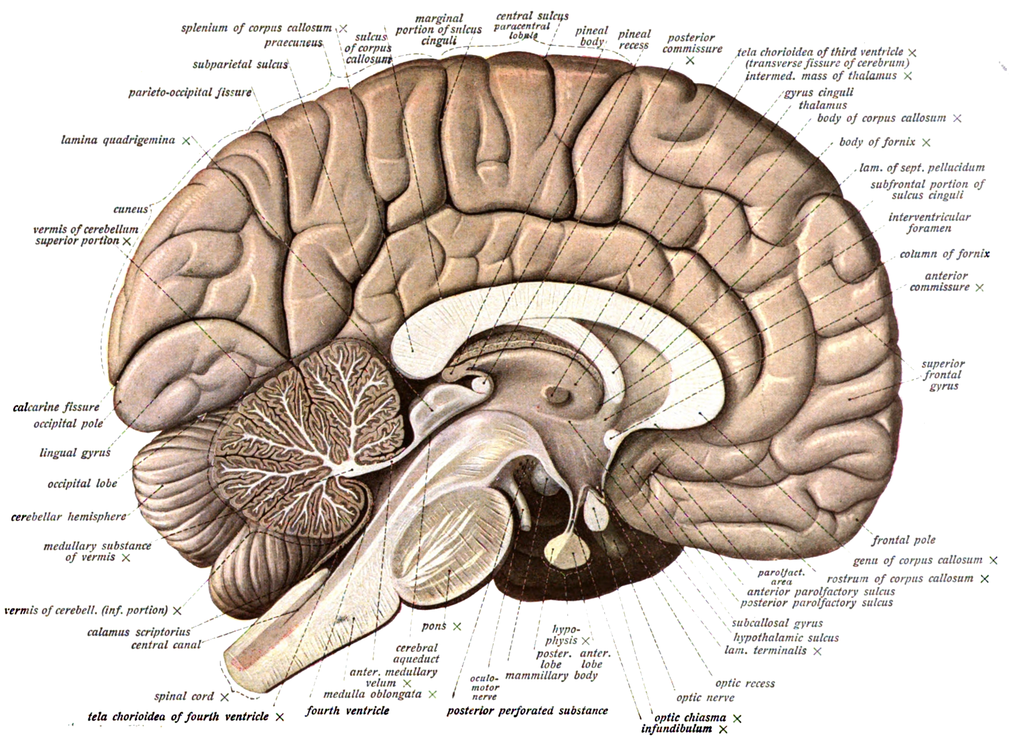
\includegraphics[width=1\textwidth]{Chapter-2/Human_brain}
    	\caption{The Human Brain (Mid-line incision view) \cite{JohannesSobotta}}
    	\label{fig:brain}
  	\end{figure}
    
	\subsection{Brain Stem}
        The Brain stem connects the brain to the spinal cord and also controls autonomic processes like breathing, digestion and heart rate.

	\subsection{Cerebellum} 
        	The Cerebellum plays an important role in balance and motor control, but is also involved in some cognitive functions such as attention, language, emotional functions and in processing and storage of memories.

 	\subsection{Cerebrum}
    	The Cerebrum is divided into two hemispheres (left and right) by the longitudinal fissure. It is also covered with a layer of neural tissues known as the Cerebral Cortex which envelops organs like thalamus, hypothalamus and pituitary glands. The Thalamus helps in relying information from the brain stem and the spinal cord to the cerebral cortex. The hypothalamus and the pituitary glands control visceral functions, body temperature and behavioral responses.  The Cerebral Cortex plays key role in memory, attention, thought, awareness, language and consciousness.
        
\section{Electroencephalography (EEG)}
\label{Electroencephalography (EEG)}
	Understanding how the brain works is a necessity in order to find solutions for various brain disorders like epilepsy, dementia, tumor etc. The methods to study the brain can be broadly classified into two methods,
    \begin{enumerate}
		\item An Invasive Approach - Requires physical implant of electrodes inside the brain.
        \item A Non-Invasive Approach - Include methods like Magnetic Resonance Imaging(MRI) and Electroencephalography.
	\end{enumerate}
    According to \cite{Kropotov}, both the methods give different perspectives and enable us to look inside the brain and observe what happens.
    
    
    Electroencephalography (EEG) was invented by a German psychiatrist, Hans Berger, who also coined the term ``Electroencephalography''. An EEG is, as defined by the Mayo Clinic, ``A test that detects electrical activity in your brain using small, flat metal discs (electrodes) attached to your scalp'' . In a healthy human brain, the brain cells (neurons), are active all the time, even while resting. As the result of these neural activities, electrical impulses are produced. What we call ``thought'' is in fact ever an changing symphony of such electrical impulses. The rhythmic neural activity in the central nervous system is popularly known as \textit{Neural Oscillation} or \textit{Brain Waves}.  For a given neuron these oscillation can occur due to rhythmic changes in the membrane potential. When these oscillations occur synchronously in a large group of neurons, macroscopic oscillations can easily be captured by EEG devices.

\section{Pattern Recognition}
	According to Charles W. Therrien \cite{Therrien:1989:DEC:61950}, `` The goal of pattern recognition is to classify objects of interest into one of a number of categories or \textit{classes}. The objects of interest are generally called \textit{patterns}''. The data used to discover the patterns is called the \textit{Training set}. The data on which the predicted pattern is tested is called the \textit{Testing set}. Pattern recognition can fall into one of the following two types,
    
    \begin{enumerate}
		\item \textbf{Supervised Pattern recognition:} If the classes of training set are known beforehand.
        \item \textbf{Unsupervised Pattern recognition or clustering:} If the classes of the training set and maybe even number the of classes are unknown before hand.
	\end{enumerate}
    
    A typical pattern recognition system is shown in Figure \ref{fig:pattern_pipeline}.
    \begin{figure}[hbtp]
        \centering
        \smartdiagram[priority descriptive diagram]{
            \centering
            Sensor,
            Pre-processing,
            Feature Extraction,
            Classifier,
            Class Assignment}
        \caption{A typical pattern recognition system}
        \label{fig:pattern_pipeline}
    \end{figure}

    
\section{Electroencephalography Sensors}
\label{Electroencephalography Sensors}
	In EEG sensors the voltage fluctuation due to the brain waves are read from the sensitive electrodes attached to the scalp. When neurons are electrically charged, electrons are either pushed to these electrodes or pulled from the electrodes and the voltage difference between any of two such electrodes can be measured by a voltmeter. Hence, EEG sensors will typically have a ground electrode, a system reference electrode along with one or more recording electrodes. In 1958, International Federation in Electroencephalography and Clinical Neurophysiology adopted standardization for electrode placement called 10-20 electrode placement system \cite{H.H.Jasper} (see Figure \ref{fig:standard}).

	There are different types of EEG sensors available, some are sophisticated and used in labs for advance research. Some sensors are available for commercial use. Notable ones are EPOC from Emotive, MUSE and MindWave from NeuroSky. More details about the commercial EEG sensors are discussed in Section \ref{Commercial EEG sensors}.

  \begin{figure}[hbtp]
    \centering
    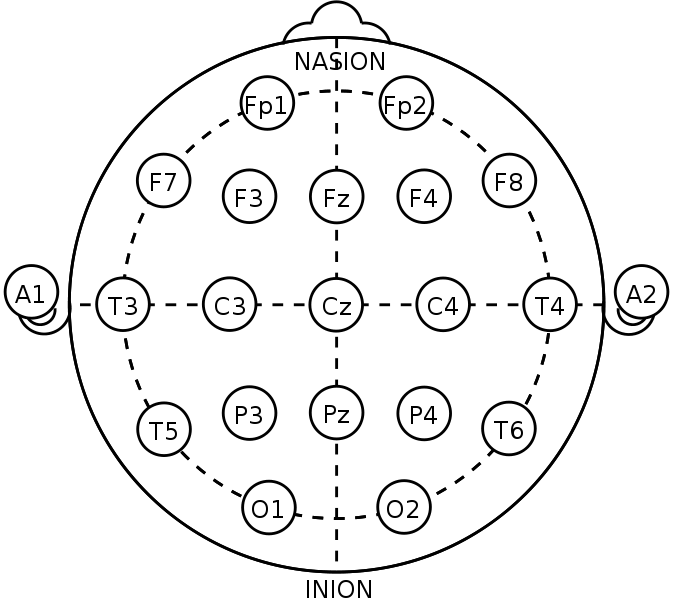
\includegraphics[width=1\textwidth]{Chapter-2/Standard}
    \caption{The 1020 System - Standardized placement of electrodes on scalp for EEG
    measurements \cite{system1020}}
    \label{fig:standard}
  \end{figure}

    \section{Raw EEG Data}
    	When an electrode in an EEG device captures the electrical activity (which occurs due to the neural activities), it also captures the electrical activity in its proximity. The captured signal also known as ``Raw EEG Data'', is a result of combination of the neural activities, electrical activity of nearby muscles and ambient noise. Generally, to reduce the effect of ambient noise, the Raw EEG Data is subjected to pre-processing methods which include digital filtering (discussed in Section \ref{Pre-processing Methods}). Also, different frequency of the raw EEG data can be linked to different brain activities. More details about EEG Frequency bands is discussed in Section \ref{EEG Frequency Bands}.
        
        
    \section{EEG Frequency Bands}
    \label{EEG Frequency Bands}
    
    The neural oscillations detected by the EEG sensors as discussed in Section \ref{Electroencephalography Sensors} are characterized by frequency, amplitude and phase. These characteristics can be extracted by time-frequency analysis. The important frequency bands associated with the brain waves are shown in the Table \ref{Table:Bands}.
    
	\begin{table}[h!]
		\centering
		\caption{EEG Frequency Bands}
		\label{Table:Bands}
		\begin{tabular}{l l}
			\hline
			Name &Frequency Band\\\hline
			Delta&0.1Hz - 4Hz\\
			Theta&4Hz - 8Hz\\
			Alpha&8Hz - 12Hz\\
			Beta&12Hz - 30Hz\\
			Gamma&30Hz - 48Hz\\
		\end{tabular}
	\end{table}

	\subsection{Delta}
    	Delta waves are low frequency waves (0.1Hz to 4Hz) generated by the brain when the individual is in deep sleep, non-REM sleep or unconscious. The delta waves are generally not detected if the individual is awake, if detected, it is either due to artificial delta waves created due to movements or due to defects in the brain.
        
	\subsection{Theta}
    	Theta waves range from 4Hz to 8Hz and are linked to Intuitive thinking, creative thinking, recall, fantasy and day dreaming. Theta waves can arise from emotional stress like frustration and disappointment \cite{YanZhang}. According to Heinrich et al.~\cite{H.H.Jasper} high level of Theta waves is considered abnormal among adults and possibly related to AD/HD.
        
	\subsection{Alpha}
    	Theta waves range from 8Hz to 12Hz and are associated with the state of relaxation while not drowsy, being tranquil and conscious.
    
    \subsection{Beta}
    	Beta waves range from 12Hz to 30Hz and are associated with performing integrative thinking, agitation, alertness, state of being relaxed yet focused and aware of self and surrounding. According to Y.Zang et al. \cite{YanZhang}, resisting or suppressing movement, or solving a math task, there is an increase of beta wave levels.
    
    \subsection{Gamma}
    	Gamma waves range from 30Hz to 48Hz and are associated with state of attention, perception, and cognition.

    \section{Commercial EEG sensors}
    \label{Commercial EEG sensors}
    Various EEG sensors are available in the market and many of them with sophisticated design are used by a doctor to examine a patient or for medical research. Figure \ref{fig:eeg_mesh} shows an example EEG sensor used in research \cite{EEGmesh}. Many EEG sensors are available for commercial use as well. EPOC from Emotive \cite{Emotive}, MUSE \cite{muse} and MindWave from NeuroSky \cite{MWMobile} are some of the notable ones.
    
	\begin{figure}[hbtp]
    	\centering
    	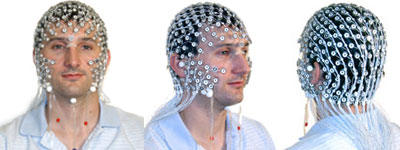
\includegraphics[width=0.9\textwidth]{Chapter-2/EEG_mesh}
    	\caption{A Geodesic Sensor Net \cite{EEGmesh}}
    	\label{fig:eeg_mesh}
  	\end{figure}
  
    	\subsection{Mindwave Mobile}
        	MindWave Mobile (shown in Figure \ref{fig:mindwavemobile}) is an EEG headset released by NeuroSky for commercial use \cite{MWMobile}. It has a recording sensor as part of the sensor arm which can be rested on forehead along with reference and ground sensors on the ear clip. The EEG data recorded from the sensors are transferred via Bluetooth to the Bluetooth enabled device like a Mac, a PC, an iPhone or an Android phone.
            
            \textbf{NOTE:} Along with the raw EEG data, MindWave Mobile can also transfer the brain wave frequency band readings, attention and meditation meters.
            
            The specifications of MindWave Mobile are as given in the Table \ref{specs}.
        \begin{table}[h!]
          \centering
          \caption{MindWave Mobile Specifications}
          \label{specs}
          \begin{tabular}{l l}
            \hline
            Parameters &Value\\\hline
            Raw EEG output & 3 to 100Hz\\
            Proprietary meters & Attention and Meditation\\
            EEG Power Spectrum & Delta, Alpha, Beta, Gamma\\
            Sampling Frequency & 512Hz\\
            Bluetooth Version&v2.1 Class 2\\
            Bluetooth Range &10m\\
            Bluetooth Pairing &Automatic\\
            Headset Type& Static\\
          \end{tabular}
        \end{table}
        
        \begin{figure}[hbtp]
            \centering
            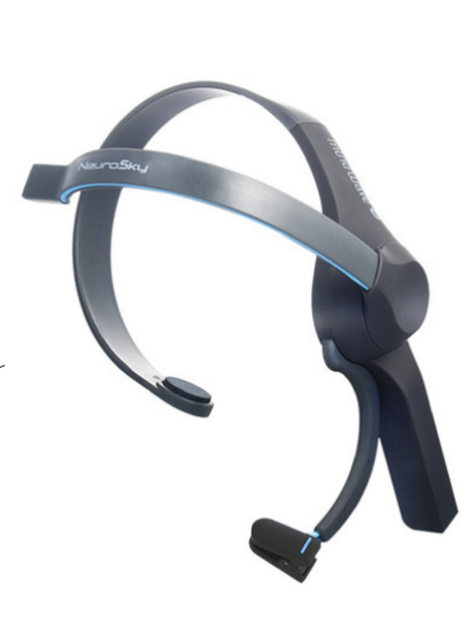
\includegraphics[width=0.9\textwidth]{Chapter-2/mindwavemobile}
            \caption{Mindwave mobile Sensor }
            \label{fig:mindwavemobile}
        \end{figure}
    
    
\section{Feature Extraction}
\label{Pre-processing Methods}
	Digital raw signal acquired from the EEG sensor are subjected to various pre-processing methods in order to extract features. These features are later used as the inputs to the classifiers. These features are generally the frequency spectrum energy bands shown in Table \ref{Table:Bands}. Multi-rate Filter banks and Fast Fourier Transform (FFT) can be used to extract the average magnitude of each spectral bands.
        
    \subsection{Fast Fourier Transforms(FFT)} 
    	The Fast Fourier Transforms (FFT) is an optimized and efficient algorithm to computer the Discrete Fourier Transform of a signal. Spectral energy of each EEG frequency band can then be calculated for each respective band of the FFT (additional details are presented in Section \ref{FeatureExtraction}).
   
\section{Classifier}
	The Classifier analyzes the feature vector (obtained by the passing prepossessed \textit{input pattern} or \textit{input vector} or \textit{measurement vector} through feature extractor) and assigns a class to the pattern. The classifier essentially induces a partitioning of the feature vector space into a number of disjoint regions \cite{Therrien:1989:DEC:61950}. Figure \ref{fig:regions} shows one such partition of the feature vector space. Here, if the feature vector falls in the region $R3$, class $c3$ is assigned to the corresponding input pattern.
    
		\begin{figure}[hbtp]
            \centering
            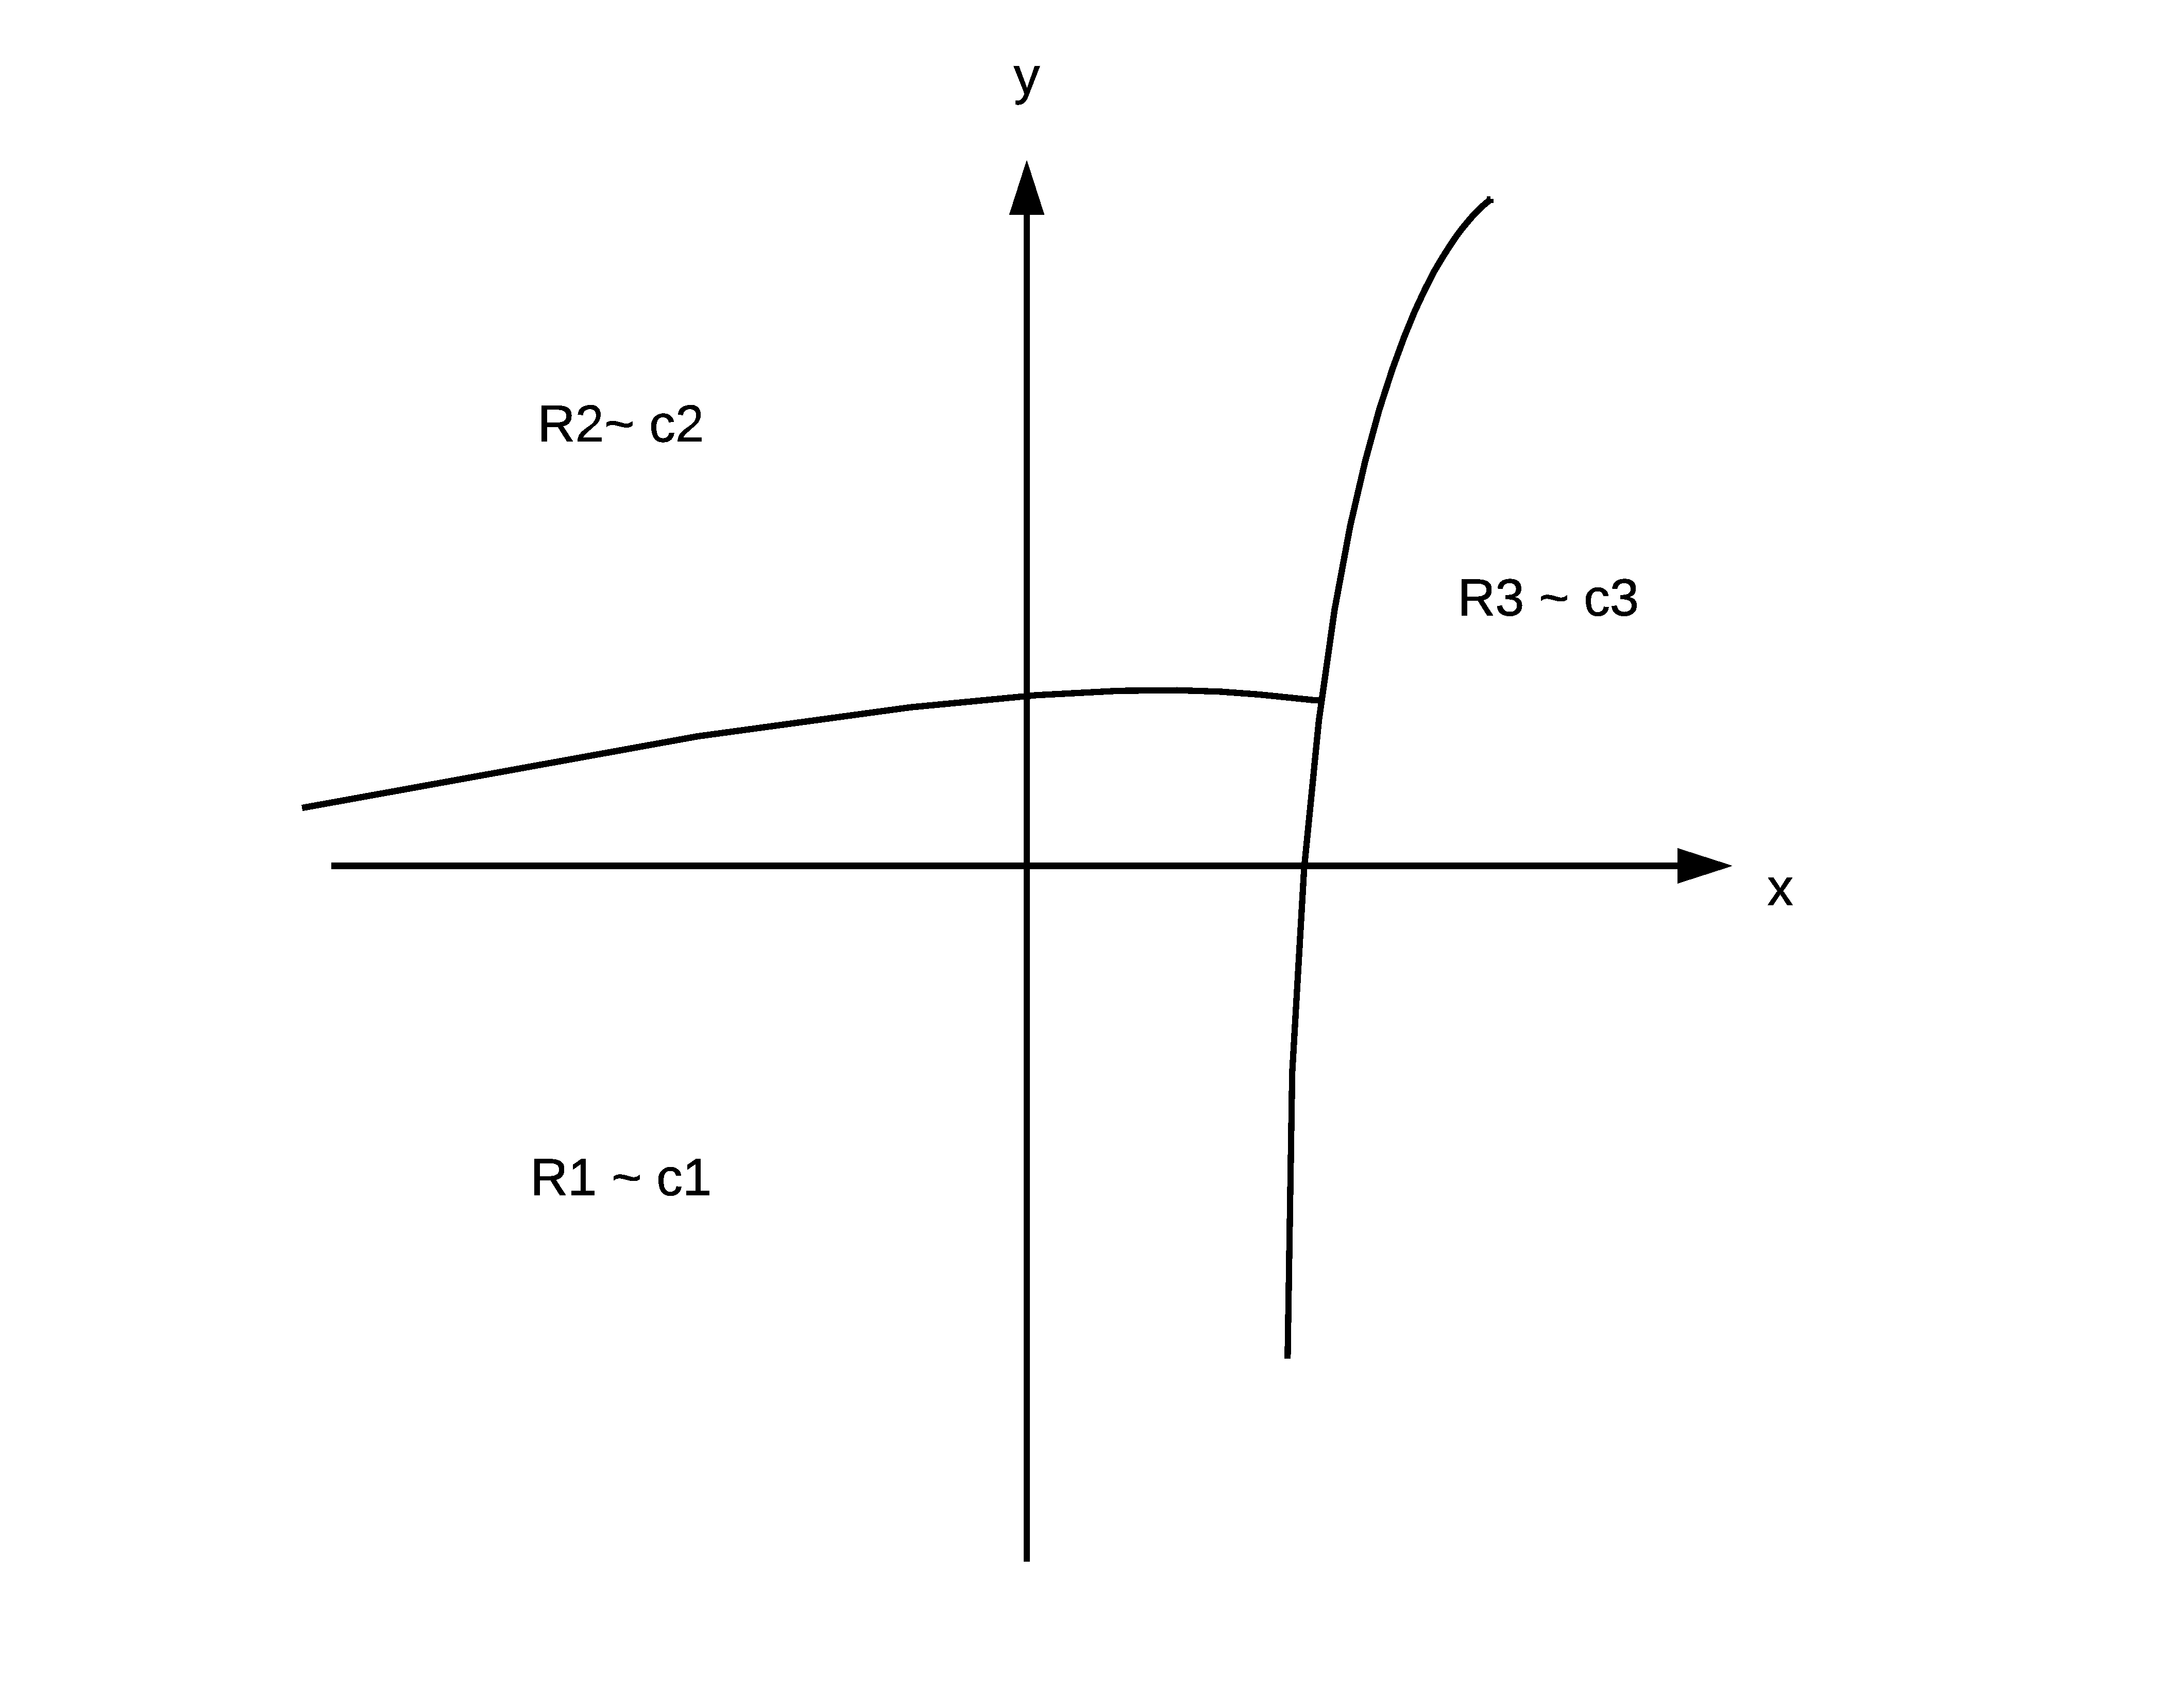
\includegraphics[width=0.9\textwidth]{Chapter-2/regions}
            \caption{Partition of feature space \cite{Therrien:1989:DEC:61950} }
            \label{fig:regions}
        \end{figure}
        
	\subsection{Mahalanobis Distance}
    \label{Chap2:Maha}
		The Mahalanobis Distance is one of the measures of distance between a feature vector and a class, it is given by Eq(\ref{Maha}).
        
		\begin{equation}
			D^2_x = (X - \mu)^T  \Sigma ^{-1}  (X - \mu)
			\label{Maha}
		\end{equation}
        
		where $D_x$ is the Mahalanobis distance, $X$ is the data vector, $\mu$ is estimated using $\mu = \frac{1}{n}\sum X$ over all the vectors in the class and $\Sigma$ is the covariance matrix of $X$. As we can see, the Mahalanobis distance is the argument of exponential of the multi-variate Gaussian Distribution that a given data vector (or feature vector) is a member of the set of vectors described by the Gaussian distribution with $\mu$ mean and $\Sigma$ covariance. \newline

		For each class $C_i$ of the training set, the mean vector $\mu_{C_i}$ and the covariance matrix $\Sigma_{C_i}$ are calculated. Using $\mu_{C_i}$ and $\Sigma_{C_i}$ of each class, the Mahalanobis Distances ($D_{XC_i}$) of the input vector $X$ in the testing set is calculated. The minimum Mahalanobis distance $D_{min}$ is then calculated using $D_{min} = min(D_{XC_i})$. The class to which the input vector $X$ belongs to is then determined by the class $C_i$ (with mean vector $\mu_{C_i}$ and the covariance matrix $\Sigma_{C_i}$) corresponding to the smallest Mahalanobis distance ($D_{min}$) for the input vector.
		
	\subsection{Artificial Neural Networks(ANN)}
    \label{Chap2:ANN}
		The Artificial Neural Networks are inspired by the behavior of biological neurons and are extensively used in machine learning field. A computational model for Neural Networks called \textit{threshold logic} was created by Warren McCulloch and Walter Pitts in 1943 \cite{McCulloch1943}. In 1958, Frank Rosenblatt created an algorithm called \textit{perceptron}, which could be used for pattern recognition \cite{Rosenblatt1958thePerceptron}. In 1975, Paul Werbos made one of the biggest advances in neural network research by creating the backpropagation algorithm \cite{werbos1974beyond}, which solved the exclusive-or issue faced by the perceptron algorithm. 
        
        An \textit{Artificial Neuron} is defined as a sum-of-products operator which produces a weighted sum of its inputs and passes it though a non-linear function such as a limiter or a sigmoid \cite{snyder2010machine} as shown in the Figure \ref{fig:ann}. An Artificial Neural Network (ANN) consists of several of such interconnected artificial neurons. A typical artificial neural network consists of an input layer, an output layer and single or many hidden layers as shown in Figure \ref{fig:nn}. Following are the types of Artificial Neural Networks.
        
        \begin{enumerate}
        	\item \textbf{Feedforward neural network -} Here the direction of data flow is from input layer to output layer and sigmoid activation is generally used.
            \item \textbf{Radial basis function network -} Here the hidden layers use Radial Basis Functions (usually Gaussian).
           	\item \textbf{Recurrent neural network -} Here the data flow can be bi-directional.
        \end{enumerate}
        
		\begin{figure}[hbtp]
			\centering
			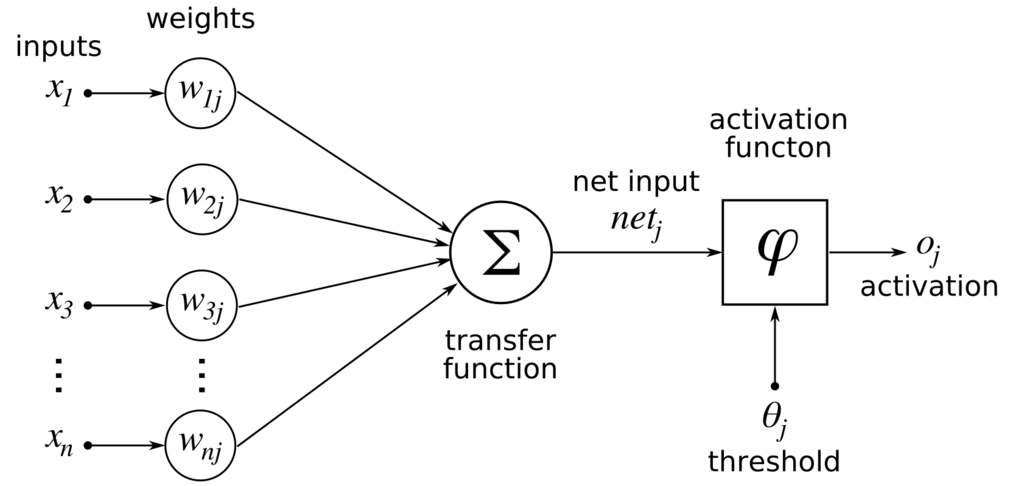
\includegraphics[width=0.9\textwidth]{Chapter-2/ann}
			\caption{An Artificial Neuron \cite{aneuronimage}}
			\label{fig:ann}
  		\end{figure}
        
        \begin{figure}[hbtp]
          \centering
          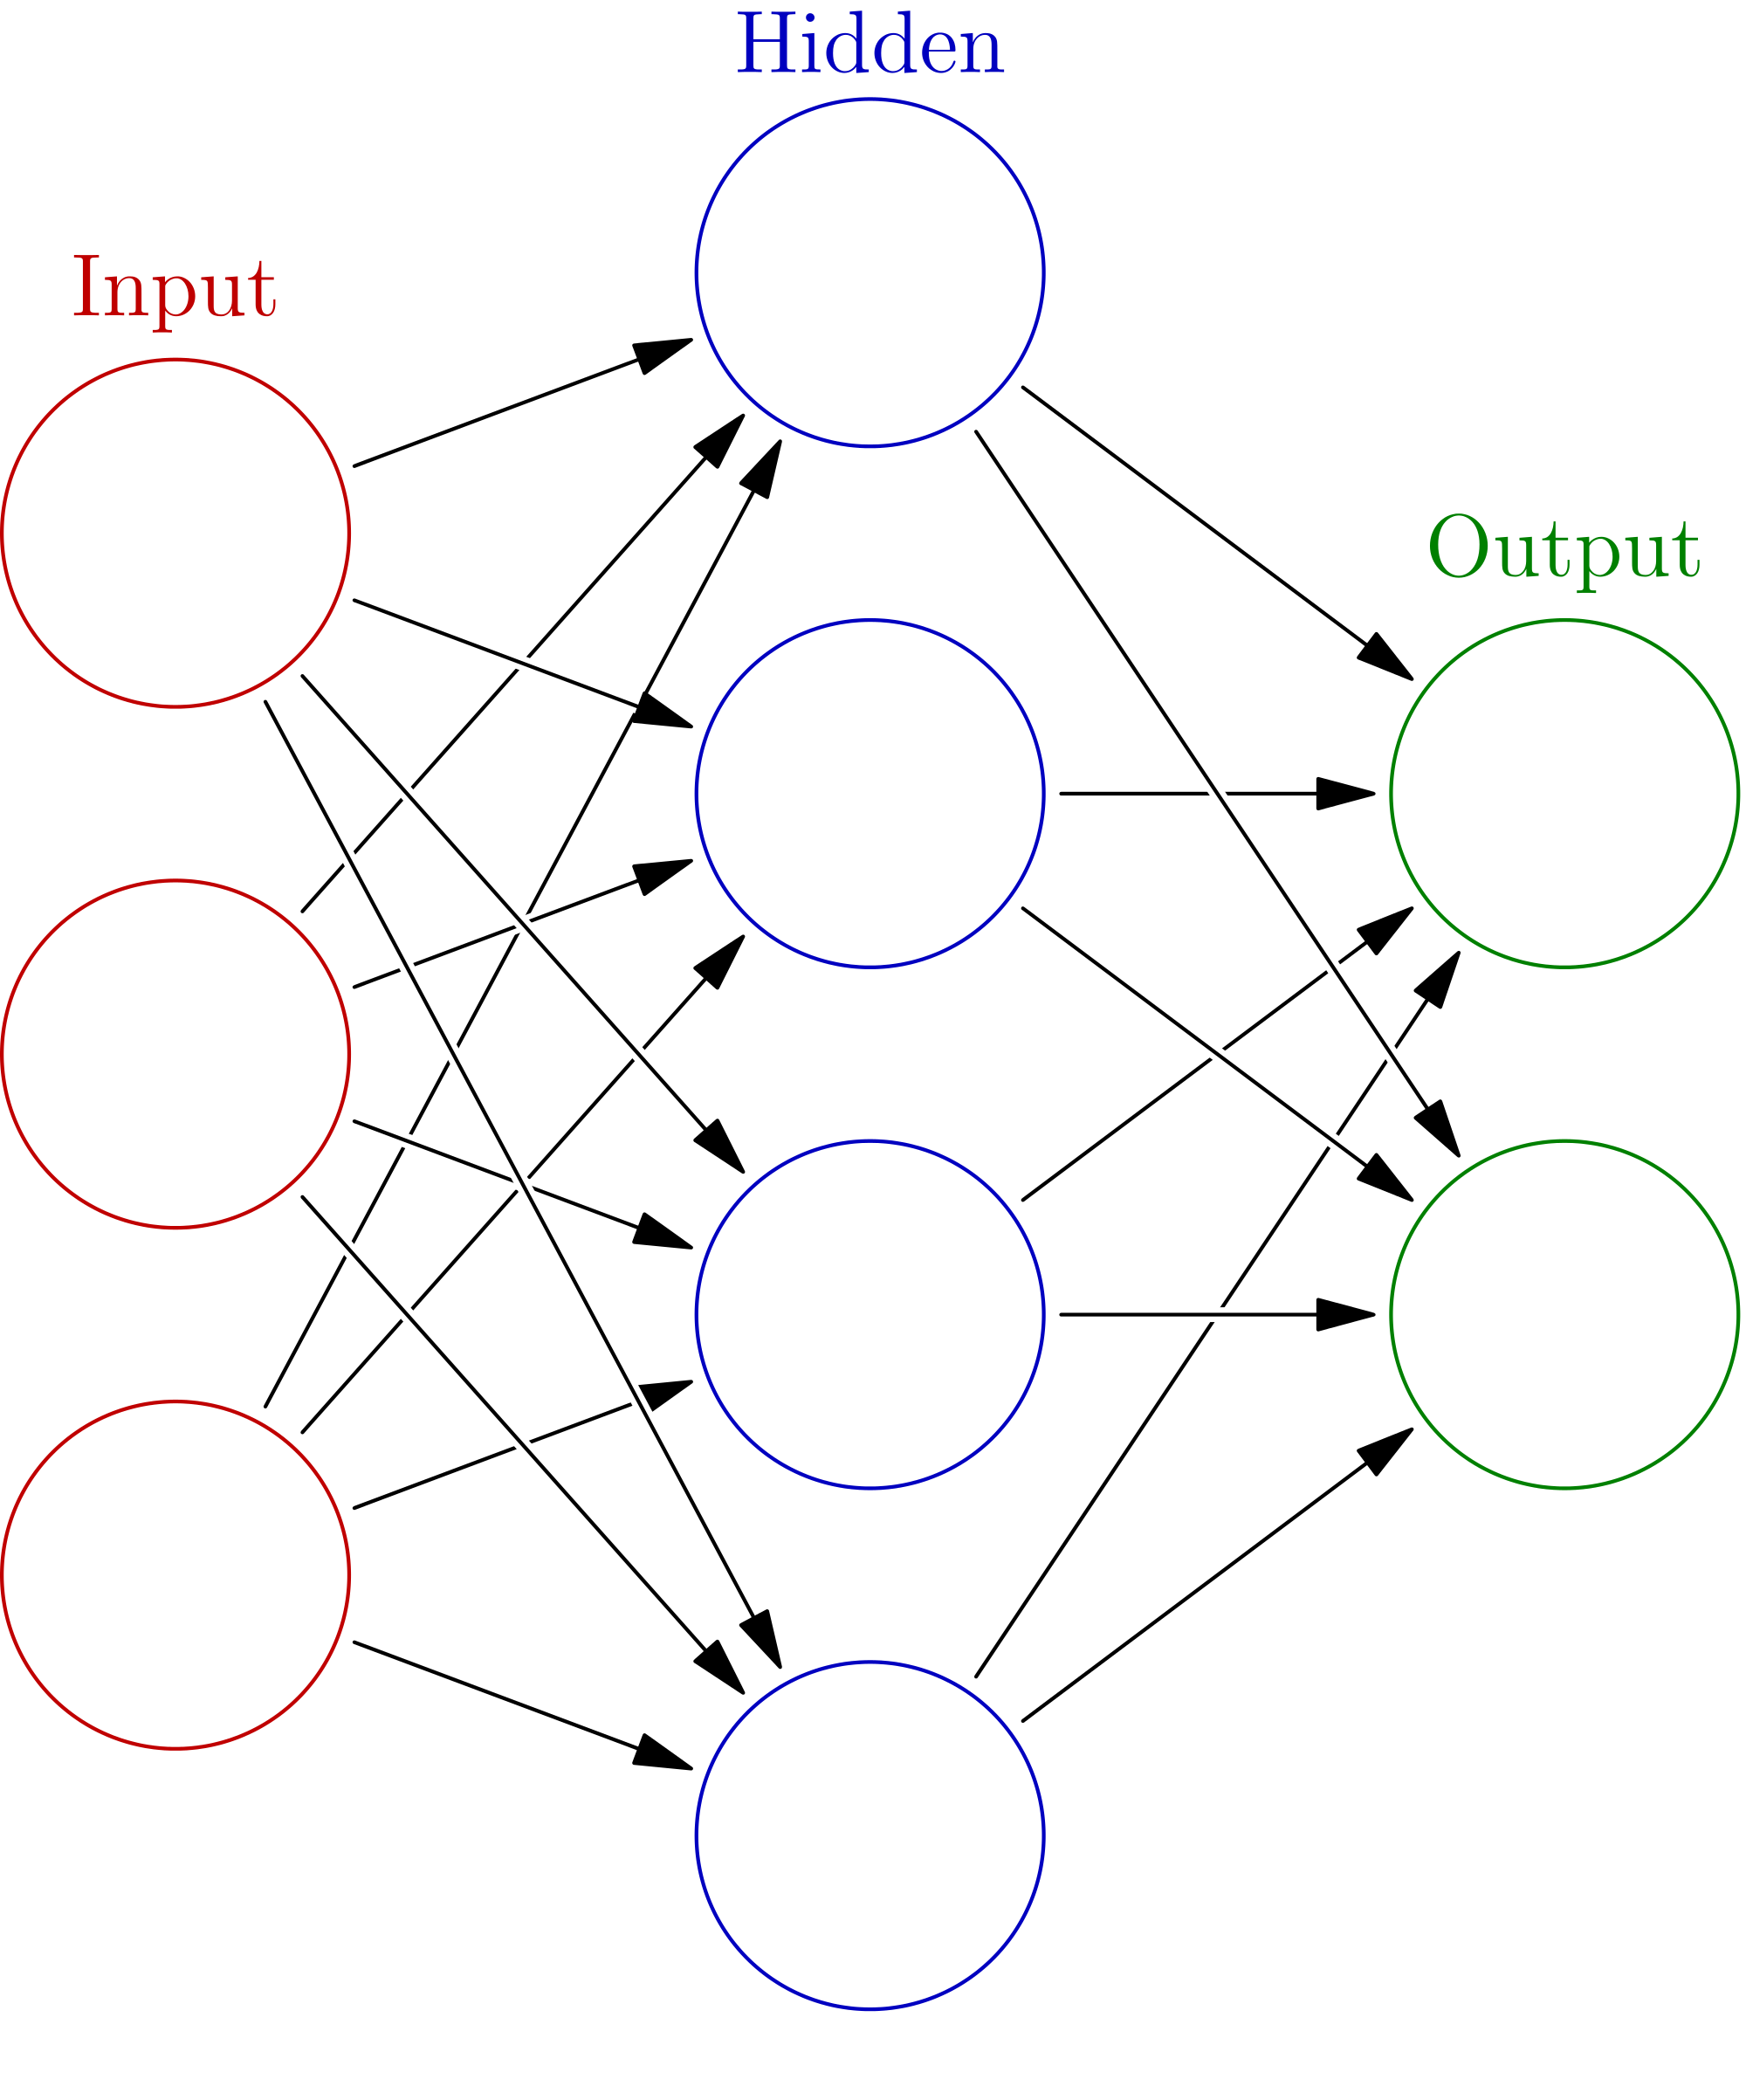
\includegraphics[width=0.6\textwidth]{Chapter-2/nn}
          \caption{A typical Artificial Neural Network with Input, Hidden and Output Layers\cite{nnimage}}
          \label{fig:nn}
  		\end{figure}
    
        In a typical feedforward neural network, the neurons in input layer are connected to the neurons in the first hidden layer and neurons in the first hidden layer are connected to the neurons in the second hidden layer and so on until the output layer. When the neural network is trained, the input activates the neurons of input layer and the activation propagates to the output layer. One of the algorithms used to train neural networks is \textit{Backpropagation} algorithm. It is an iterative algorithm which trains the neural network and adjusts the network parameters by minimizing the output error. More details about the Neural Networks and the backpropagation algorithm is discussed in Section \ref{Artificial Neural Networks}.

	\subsection{Support Vector Machines (SVM)}
    \label{chap2:SVM}
		The Support vector machines is one of the supervised learning models used in machine learning introduced by Vapnik \cite{Boser:1992:TAO:130385.130401}. The SVMs preprocess the m-dimensional input vector to represent patterns in a n-dimension space - typically $n>>m$. With an appropriate non-linear mapping function to a sufficiently higher dimension, data from two categories can be separated by a hyperplane \cite{duda2001pattern}. Say if we have class $C_1$ and $C_2$ which are separable by a hyperplane. Let, $d_1$ be the distance between closest point of $C_1$ and the hyperplane. Similarly, let $d_2$ be the distance between closest point of $C_2$ and the hyperplane. The \textit{margin} is defined as $d_1 + d_2$. Support Vector Machines can be seen as an optimization problem which minimize the margin \cite{snyder2010machine} (See Figure \ref{fig:badsvm} and Figure \ref{fig:goodsvm} for a non-optimal and an optimal choice of dividing hyperplane in 2D).
        
        \begin{figure}[hbtp]
            \centering
            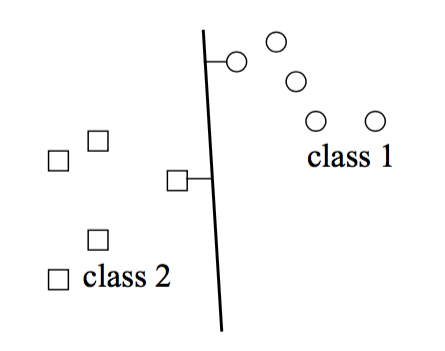
\includegraphics[width=0.6\textwidth]{Chapter-2/badsvm}
            \caption{Non-optimal dividing hyperplane \cite{snyder2010machine}}
            \label{fig:badsvm}
  		\end{figure}
        \begin{figure}[hbtp]
            \centering
            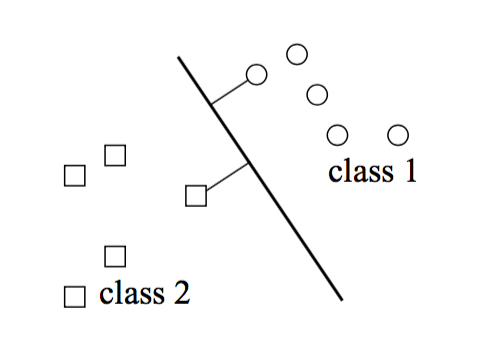
\includegraphics[width=0.6\textwidth]{Chapter-2/goodsvm}
            \caption{Optimal dividing hyperplane \cite{snyder2010machine}}
            \label{fig:goodsvm}
  		\end{figure} 
        
        Since SVMs deal with separating the input data into two by a hyperplane, it is suitable for binary classification, in fact, SVMs can be seen as a non-probabilistic binary linear classifiers. However, multi-class classification can be done by reducing the multi-class classification problem into many binary classification problems. For example, one-vs-rest or one-vs-all is one of the methods used for this. In one-vs-all classification method, a series of binary classifiers are built which distinguish between one class and the rest. The classes are then assigned using winner-take-it-all strategy. Section \ref{Support Vector Machines} discusses about the Support Vector Machines in greater detail.
        
        \section{Conclusion}
        	In Chapter \ref{chap-two}, we discussed about security, security typed, usage of EEG in security and methods used to achieve the same using pattern recognition methods. In Chapter \ref{chap-three}, we will discuss in more detail about the design and methodology of pattern recognition pipeline of a security system using EEG.
        
\ensureoddstart
\chapter{METHODOLOGY}
\label{chap-three}

	EEG data for three different mental tasks were collected from four different test subjects. The three mental tasks are as shown in Table \ref{Tasks}. Each mental task was carried out for ten seconds and repeated five times comprising fifty seconds duration of EEG signal for each task. During each task the subjects were asked to sit on a chair, close their eyes and restrict any muscle movements. The raw EEG data collected from the EEG sensor was then passed through pre-processing block, feature extraction block and classifier block consecutively. Figure \ref{fig:FlowChart} shows the overall flow of data from the EEG sensors to classifier.
		\begin{figure}[hbtp]
            \centering
            \smartdiagram[priority descriptive diagram]{
                \centering
                EEG Sensor,
                Pre-processing (Filtering),
                Feature Extraction (Spectral Energy of EEG bands),
                Classification,
                Class Assignment}
    		\caption{Overview of User Verification System using EEG}
    		\label{fig:FlowChart}
    	\end{figure}
        
		\begin{table}[h]
			\centering
			\caption{Mental Tasks}
			\label{Tasks}
			\begin{tabular}{l l}
				\hline
				Task &Description\\\hline
				Calculating&Performing a mental calculation of two digit multiplication\\
				Breathing&Concentrating on breathing\\
				Singing&Mentally singing a song without actually singing out loud\\
			\end{tabular}
		\end{table}
    
    
\section{Pre-Processing}
	The data stream was read at 512 samples per second from MindWave Mobile EEG sensor and stored in a file. Different files were used for each user, each mental task and each repetition of the mental task. The stored raw EEG data was then passed through a band-pass filter to eliminate unnecessary frequency bands. If total number of samples for each repetition of a mental task for a given user was $n$, then the filtered data $X'=[x_1', x_2', \ldots, x_n']^T$ was obtained by passing $X=[x_1, x_2, \ldots, x_n]^T$ through the band pass filter $F$ as shown in Equation \ref{EQ:bpf}. The lower cutoff frequency and the higher cutoff frequency for the band pass filter were 0.1Hz and 48Hz respectively.
    
    \begin{equation}
		\label{EQ:bpf}
        X' = F(X) \;.
	\end{equation}
    
    The filtered data were then divided into subgroups, each subgroup with one second data. Say, if ten seconds of EEG readings were recorded, the total samples of raw EEG data stored in the file would be $512\times 10=5120$. Each sub group would contain $512\times1=512$ samples. And total number of sub groups would be $5120\div512=10$. Say, if EEG readings for user $i$ were collected for mental task $j$, repeated for $k^{th}$ time, then the filtered EEG data for sub group $l$ is given by Equation \ref{EQ:subGrp}.
    \begin{equation}
		\label{EQ:subGrp}
        X_{ijkl}' = [x_1', x_2', \ldots ,x_{511}', x_{512}']^T \;.
	\end{equation}
    
\section{Feature Extraction}
\label{FeatureExtraction}
	As discussed in Section \ref{EEG Frequency Bands} neural activities can be characterized by frequencies. Table \ref{Table:Bands} shows different EEG frequency bands and their frequency ranges. Since different brain activities result in different energy levels of EEG frequency bands, using spectral energy of EEG frequency bands as input feature vectors to the classifier is an excellent choice. In order to increase the dimension of input vectors, some of the EEG frequency bands were further sub-divided into low and high bands, resulting in eight EEG frequency bands as show in Table \ref{Table:Bands_more} (also see Figure \ref{fig:eeg_bands}).
    
    	\begin{table}[h!]
		\centering
		\caption{Frequency Bands used for Feature extraction}
		\label{Table:Bands_more}
		\begin{tabular}{l l}
			\hline
			Name &Frequency Band\\\hline
			Delta&0.1Hz - 4Hz\\
			Theta&4Hz - 8Hz\\
            Low Alpha&8Hz - 10Hz\\
			High Alpha&10Hz - 12Hz\\
            Low Beta&12Hz - 18Hz\\
			High Beta&18Hz - 30Hz\\
            Low Gamma&30Hz - 40Hz\\
			High Gamma&40Hz - 48Hz\\
		\end{tabular}
	\end{table}


	\begin{figure}[hbtp]
    	\centering
    	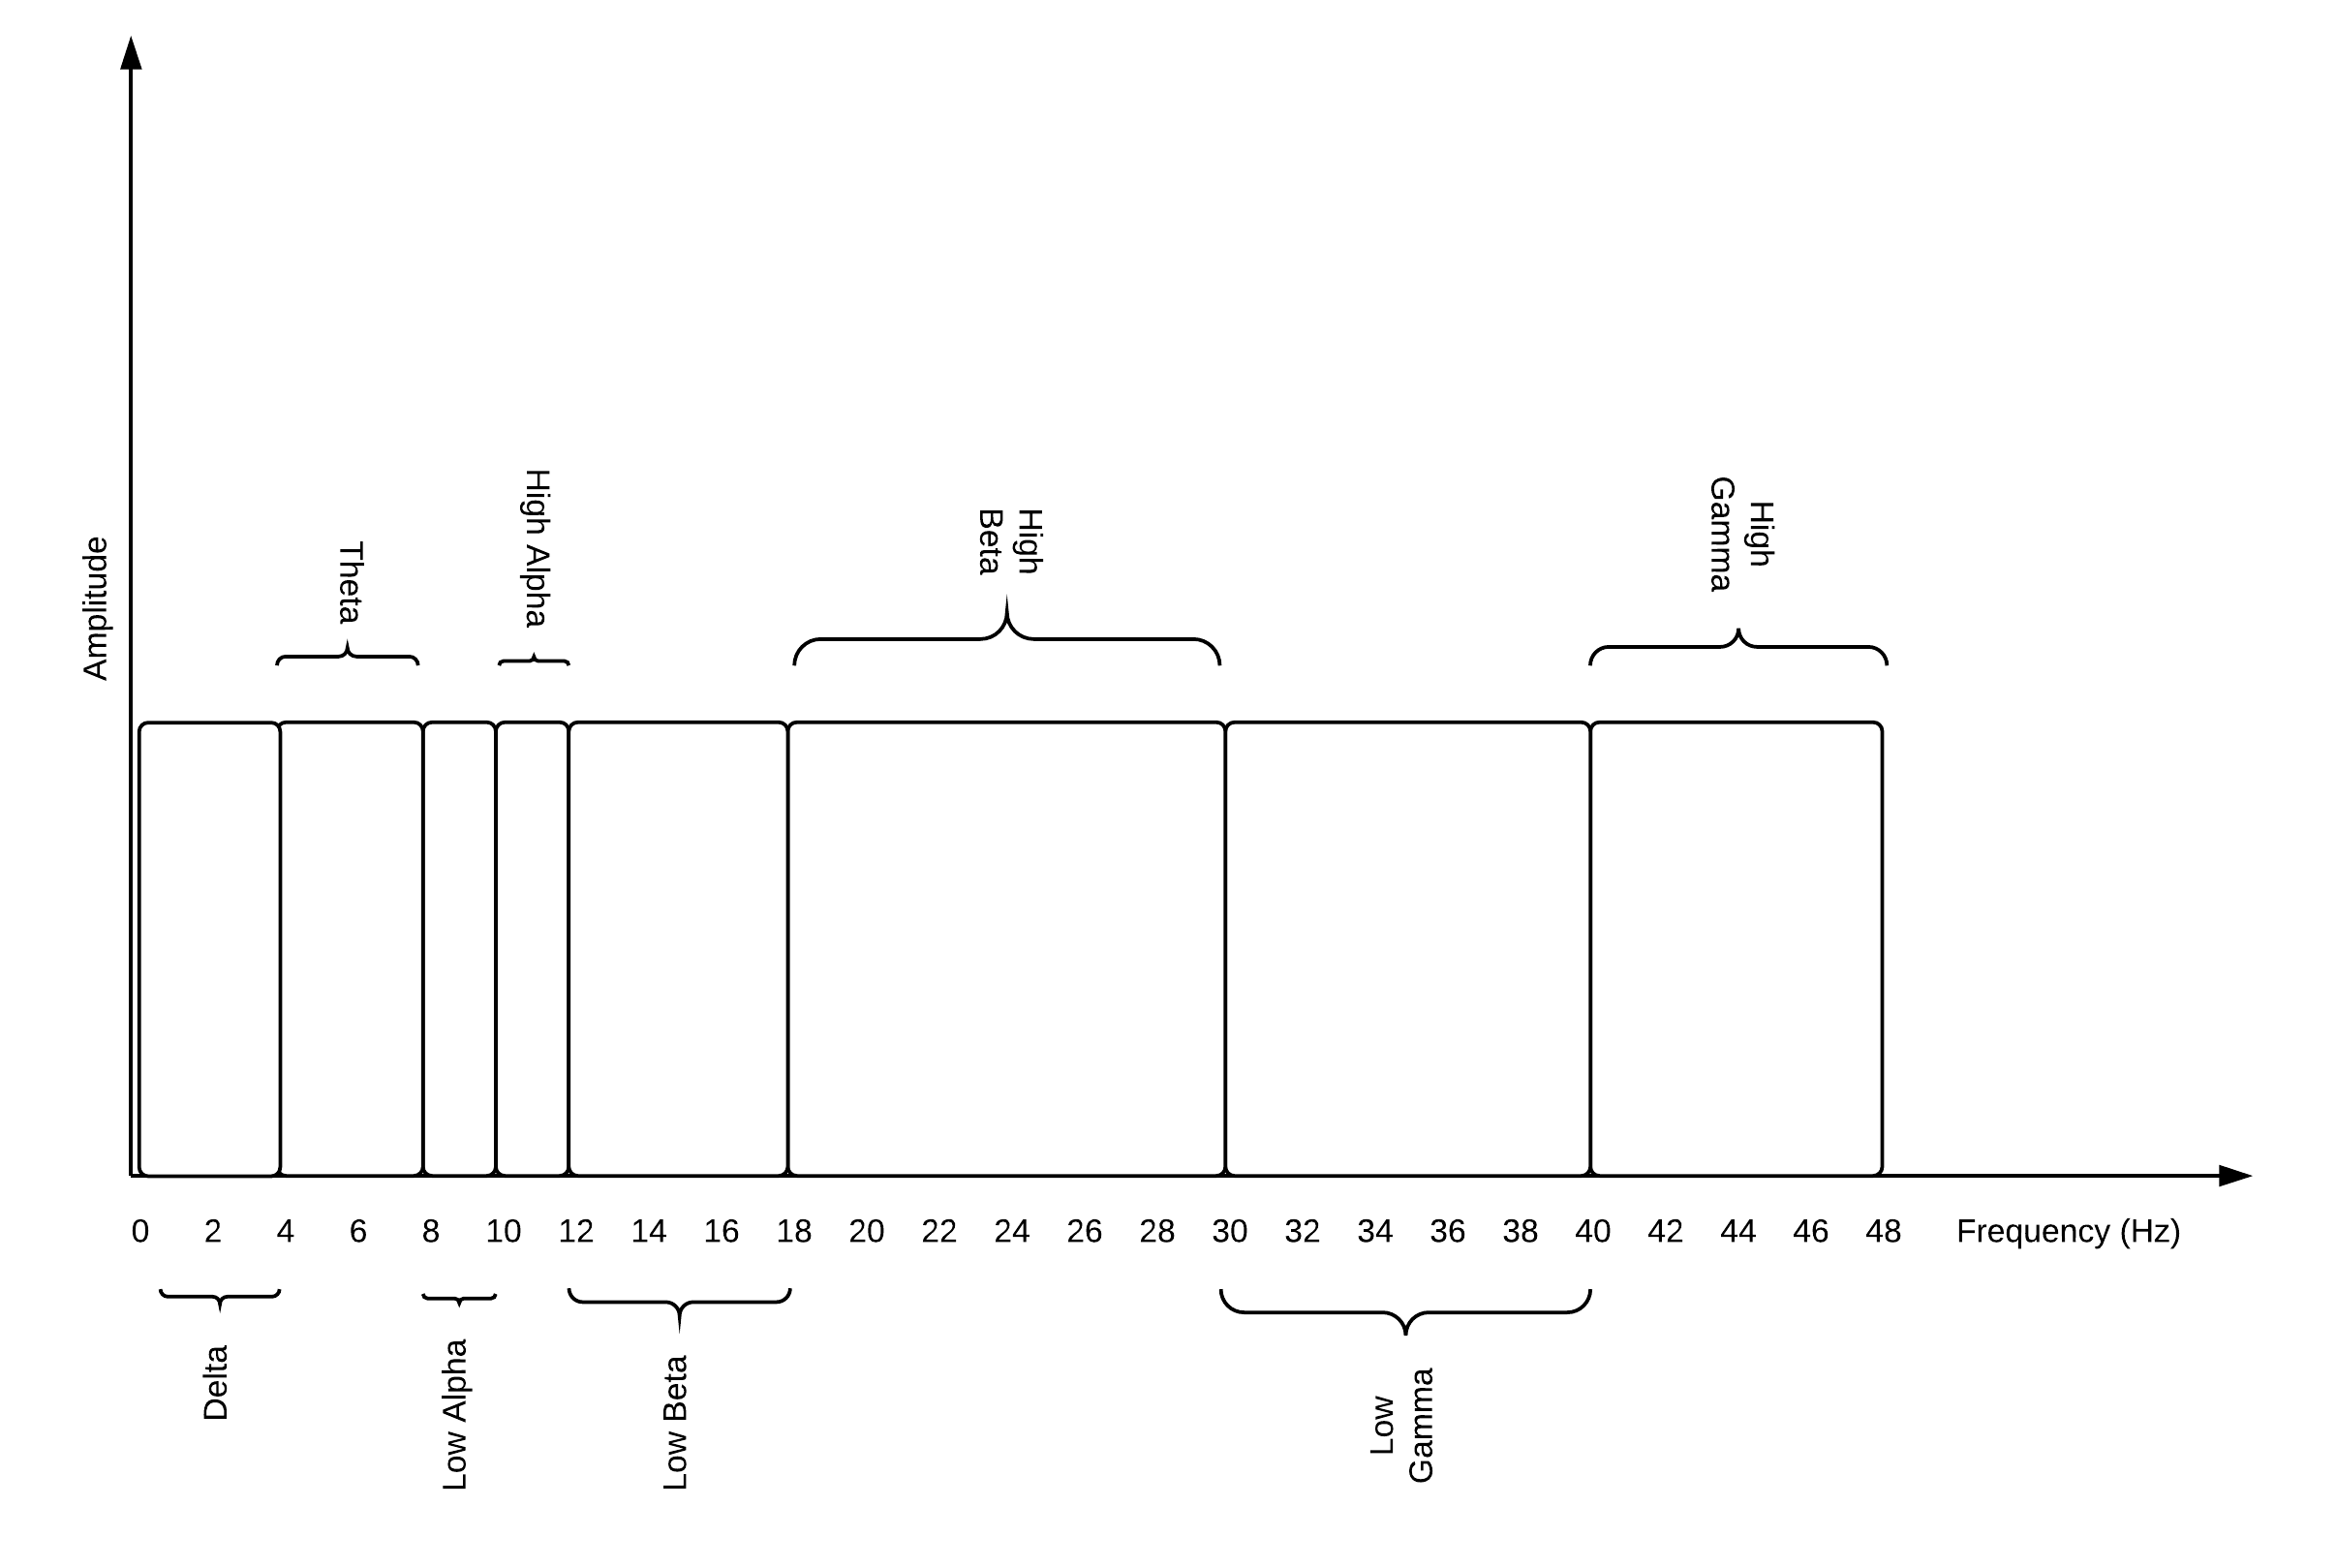
\includegraphics[width=1\textwidth]{Chapter-3/EEG_bands}
    	\caption{EEG Frequency Bands}
    	\label{fig:eeg_bands}
  	\end{figure}
    
	First, we pass the each subgroup of filtered EEG data(containing 512 samples) through the 512 point Discrete Fourier Transform (DFT) block and obtain their DFT.
    
    If $X(n)$ is the input data sequence, $\mathscr{F}$ is the DFT operation and $X_k$ is the DFT of $X(n)$, Equation \ref{EQ:time_to_dft} symbolically shows the DFT operation conducted on input sequence $X(n)$.
    
    \begin{equation}
    	X(n) \xrightarrow{\mathscr{F}} X_k \;.
        \label{EQ:time_to_dft}
    \end{equation}
    
    Say, if each subgroup of filtered EEG samples is $X(n) = [x_1, x_2, \ldots, x_{512}]^T$ and the DFT of $X(n)$ is $X(k)$, then the 512 point DFT of $X(n)$ is given by Equation \ref{EQ:dft}.
    
    
    \begin{equation}
    	X(k) = \sum_{n = 0}^{n = 511}{X(n) \cdot \exp{(-2 \pi i k n/512)}}, k \epsilon Z \;.
		\label{EQ:dft}
    \end{equation}
    
    The spectral energy of each EEG frequency band $i$ may be calculated using Equation \ref{EQ:spectral_energy}.
    
    \begin{equation}
    	E_i = \sqrt{\frac{1}{m_2 - m_1 + 1} \sum_{k=m_1}^{k=m_2} \left | X(k) \right | ^2} \;,
    	\label{EQ:spectral_energy}
    \end{equation}
    
    \noindent where $m_2$ > $m_1$ and $k=[m_1,m_2] \in $ EEG frequency band $i$.
    
    After obtaining the spectral energy of each EEG frequency band, we combine them to form a vector as shown in Equation \ref{EQ:in_vectors}.
    
    \begin{equation}
    	X_{in} = [E_1, E_2, \ldots E_8] \;.
    	\label{EQ:in_vectors}
    \end{equation}
    
    We then normalize the EEG spectral energy band vector $X_{in}$ as shown in Equation \ref{EQ:norm} to obtain an unit vector $X_{n}$. This is next used as the input for the classifiers discussed in Section \ref{Chap3:Classifiers}. Note that by normalizing, we were able to neutralize the effect of different sensitivity levels of EEG sensor for different users and test cases.
   
	\begin{equation}
    	X_{n} = \frac{1}{\left | X_{in} \right |} X_{in} \;.
    	\label{EQ:norm}
    \end{equation}
    
\section{Classifiers}
\label{Chap3:Classifiers}

		The input feature vectors obtained from the pre-processing block were randomly shuffled and split into training and testing. Following is the training and testing split percentage, 
		\begin{enumerate} 
			\item 70\% of the feature vectors data set were used as training set.
			\item 30\% of the feature vectors data set were used as testing set.
		\end{enumerate}
		For example, if each EEG mental task experiment (lasting 10 second each) is repeated 5 times, we have raw EEG data of 50 seconds. After pre-processing this data, we will have 50 input feature vectors. We then shuffle the ordering of these vectors and pick 35 (70\%) as part of training set and 15 (30\%) as part of testing set. The shuffling is done to randomize the training and testing split.
        
        Since we have different users performing many mental tasks, we can try to identify the mental task given the subject or we can try to identify the subject among many subjects given the mental task. For this reason, we have conducted two different types of classification as given below,
        
		\begin{enumerate}
			\item \textbf{Intra - Subject Classification} : Identifying a mental task in a set of mental tasks performed by a single subject.
			\item \textbf{Inter - Subject Classification} : Identifying a subject in a set of subjects performing the same mental task.
		\end{enumerate}
        
\subsection{Mahalanobis Distance}
\label{Mahalanobis Distance}
	As discussed in \ref{Chap2:Maha}, the Mahalanobis Distance is a simple pattern recognition technique used to identify the class of the input vector. In our case, a class is either the type of task or the subject performing the mental task depending on the the classification type. The input vector $\mathbf{x}$ is the pre-processed EEG data vector given by Equation \ref{EQ:chap3X}.

	\begin{equation}
    	\mathbf{x} = [x_1\quad x_2 \ldots x_N] \;,
    	\label{EQ:chap3X}
    \end{equation}
    \noindent where $N$ is the number of variable in the input vector $\mathbf{x}$.
	
    The Mahalanobis distance is computed using the Equation \ref{EQ:chap3Maha}.
	\begin{equation}
    	D^2_x = (\mathbf{x} - E[\mathbf{x}])^T \bm{\Sigma}^{-1} (\mathbf{x} - E[\mathbf{x}]) \;,
    	\label{EQ:chap3Maha}
    \end{equation}
    
    \noindent where $\bm{\Sigma} ^{-1}$ is the inverse of the covariance matrix $\Sigma$ and $E[\mathbf{x}]$ is the expected value of $\mathbf{x}$.
    
    The expected value of $\mathbf{x}$ is given by Equation \ref{EQ:chap3Mean}.

	\begin{equation}
		E[\mathbf{x}] = \bm{\mu} = [\mu_1 \mu_2 \ldots \mu_N] = \sum_{i=1}^{M}\mathbf{x}_i \;,
    	\label{EQ:chap3Mean}
    \end{equation}
    
    \noindent where M is the number of input vectors.
    
    The covariance matrix $\bm{\Sigma}$ is given by Equation \ref{EQ:chap3Cov}.
	\begin{equation}
		\bm{\Sigma} = [(E[\mathbf{x} - E[\mathbf{x}])(E[\mathbf{x} - E[\mathbf{x}])^T ]
    	\label{EQ:chap3Cov}
    \end{equation}    
    
 %   However, since estimate of all possible samples is not feasible, we compute the estimate of covariance %matrix using sample covariance matrix given by Equation \ref{EQ:chap3SampleCovEle}
 %   
 %   \begin{equation}
 %   	\bm{\Sigma} = \begin{bmatrix}
 %   				\Sigma_{11} & \Sigma_{12}  & \ldots & \Sigma_{1j} \\
 %   				\Sigma_{21} & \Sigma_{22}  & \ldots & x_{2j} \\
 %   				\vdots 	    & \vdots       & \ldots & \vdots\\
 %   				\Sigma_{i1} & \Sigma_{i2}  & \ldots & \Sigma_{ij}
%\end{bmatrix}
%    	\label{EQ:chap3SampleCov}
%    \end{equation}
%    
%    Here the sample covariance of each element i,j is computed as given in Equation 
%\ref{EQ:chap3SampleCovEle}
%   
%    \begin{equation}
%    	\bm{\Sigma}_{ij} = \frac{1}{N} \sum_{k=1}^{N} (F_i(k) - \mu_i)(F_j(k) - \mu_j)
%    	\label{EQ:chap3SampleCovEle}
%    \end{equation}
%    
%    where $N$ is the number of samples in feature $F_i$ and $\mu_i$ is given by Equation 
%\ref{EQ:chap3SampleMean}.
%   
%    \begin{equation}
%		\mu_i = \frac{1}{N} \sum_{k=1}^N F_i(k)
%    	\label{EQ:chap3SampleMean}
%    \end{equation}    
    
    As discussed in \ref{Chap2:Maha}, we first calculate the mean vectors and sample covariance matrices for all the classes in the training set. We then calculate the Mahalanobis distance of the input testing vector with respect to each and every class using their corresponding mean vector and sample covariance matrix. We then assign the class label to the input testing vector by computing ``the class which gives smallest Mahalanobis distance''. Say, if we have class $C_1, C_2 \ldots , C_m$ and $d_1, d_2 \ldots d_m$ are the corresponding Mahalanobis distances of an input testing vector, we assign this input vector the class label $C_i$, if $d_i = min(d_1, d_2 \ldots , d_m)$. Similarly, we then classify every single input in the testing set using Mahalanobis Distance.  
    
\subsection{Artificial Neural Networks}
\label{Artificial Neural Networks}
 
 	In Section \ref{Chap2:ANN}, we briefly discussed Artificial Neural networks and how they can be used in pattern recognition. In this section, we will discuss perceptrons and multiple layer feed forward neural network.
    
    \subsubsection{Perceptron}
    
    \begin{figure}[hbtp]
    	\centering
    	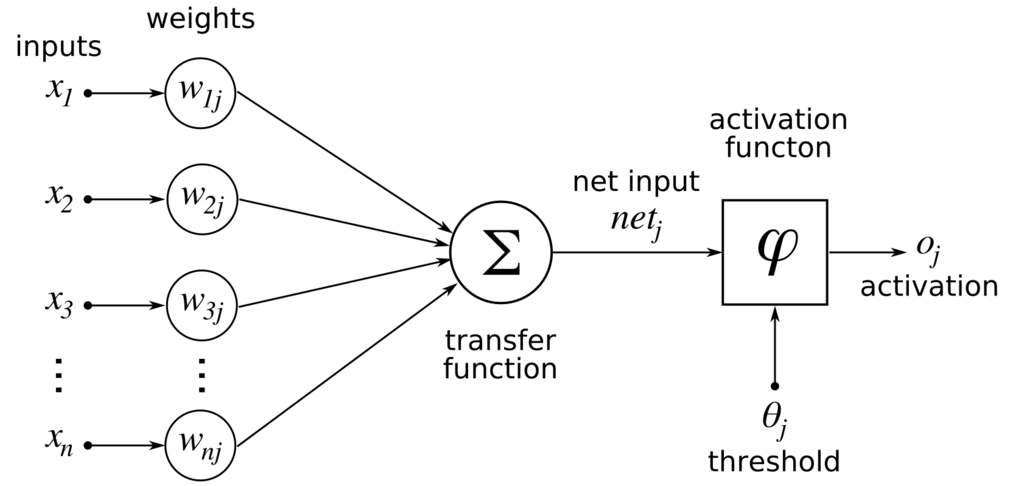
\includegraphics[width=0.9\textwidth]{Chapter-2/ann}
    	\caption{Perceptron \cite{aneuronimage}}
    	\label{fig:chap3ann}
    \end{figure}
    
    Consider Figure \ref{fig:chap3ann}, where input $\bm{x}$ and weights of the perceptron $\mathbf{w}$ are given by Equation \ref{EQ:chap3input} and Equation \ref{EQ:chap3weights} respectively. Perceptron uses the input vector $\mathbf{x}$ and weight vector $\mathbf{w}$ such that the classification boundary, $\mathbf{w}^T\mathbf{x} = 0$ separates the classes.
    
    
    \begin{equation}
    	\mathbf{x} = [1 x_1 x_2 x_3 \ldots x_m]^T \;.
        \label{EQ:chap3input}
    \end{equation}    
	\begin{equation}
    	\mathbf{w} = [w_0 w_1 w_2 \ldots w_m]^T \;.
        \label{EQ:chap3weights}
    \end{equation}

	The output of the perceptron for a given input vector is calculated using Equation \ref{EQ:chap3PerOut}.
    
    \begin{equation}
    	F(\mathbf{x}) = \varphi(\mathbf{w}^T\mathbf{x}) \;,
		\label{EQ:chap3PerOut}
    \end{equation}
        
	\noindent where $\varphi$ is the activation function. Different activation function like tanh (Equation \ref{EQ:chap3tanh}), sigmoid (soft step) (Equation \ref{EQ:chap3softstep}) etc., can be used as activation function. The choice of the activation function does not affect the training methods. For our experiments we use sigmoid activation function.
    
    \begin{equation}
    	\varphi(v) = \frac{e^v - e^{-v}}{e^v + e^{-v}} \;.
    	\label{EQ:chap3tanh}
    \end{equation}
    \begin{equation}
		\varphi(v) = \frac{1}{1 + e^{-v}} \;.
    	\label{EQ:chap3softstep}
    \end{equation}        
        
        
        Since the perceptron is a supervised machine learning algorithm, it requires training. Here, the training involves tuning the weight vector $\mathbf{w}$. This can be done using the Gradient Decent algorithm. If $d_j$ represents the desired output and $y_j$ is the actual output of the perceptron for $j^{th}$ input vector $x_j$, we can calculate the error function for $i^{th}$ iteration of the gradient decent algorithm using Equation \ref{EQ:chap3Grad}.
        
        \begin{equation}
        	E^{(i)} = \frac{1}{2m}\sum_{k =1}^{k = m} (\varphi(\mathbf{w}^T x(k)) - d(k))^2 \;.
        	\label{EQ:chap3Grad}
        \end{equation}
        
        The Gradient Decent Algorithm states that, the error function $E$ can be minimized (given that $\varphi(\mathbf{w}^T x(k))$ is differentiable) by updating the weight vector as shown in Equation \ref{EQ:chap3GradUpdate}.
        
        
        \begin{equation}
        	\mathbf{w}^{(i + 1)} = \mathbf{w}^{(i)} - \eta \cdot \mathbf{x} \cdot (\mathbf{y}^{(i)} - \mathbf{d}) \;,
        	\label{EQ:chap3GradUpdate}        
        \end{equation}
        
        \noindent where $\mathbf{y} = [y_1 y_2 \ldots y_n]^T$ is the actual output of the perceptron in vector form, $\mathbf{d} = [d_1 d_2 \ldots d_n]^T$ is the desired output of the perceptron in vector form and $\eta$ is the learning rate parameter. The learning rate parameter $\eta$ determines how fast the weights converge. Keeping $\eta$ too low will result in slow convergence resulting in large number of iterations to reach the optimal solution. On the other hand, large $\eta$ might not guarantee the optimal solution. Hence, it is better to start $\eta$ with a high value and gradually reduce it after every iteration.
        
        \subsubsection{Multi Layer Perceptron}
        
        The Multi layer perceptron (MLP) is an extension of the perceptron. This architecture has more neurons connected to each other and allows  non-linear classification boundaries. As discussed in Section \ref{Chap2:ANN}, the multi layer perceptron typically contains an input layer, one or more hidden layers and an output layer as shown in Figure \ref{fig:chap3mult} . 

    \begin{figure}[hbtp]
    	\centering
    	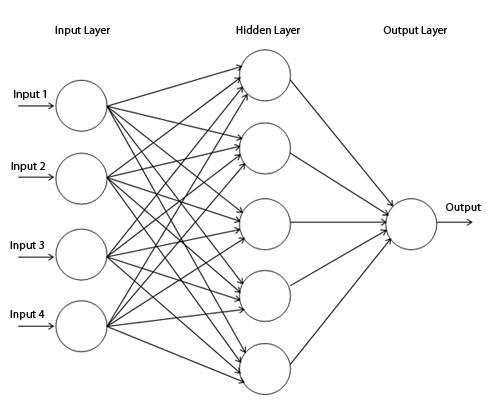
\includegraphics[width=0.9\textwidth]{Chapter-3/mult}
    	\caption{Multi Layer Perceptron \cite{multipercep}}
    	\label{fig:chap3mult}
    \end{figure}
    
        According to Universal approximation theorem, a single hidden layer with finite number of neurons is sufficient to approximate a given training set \cite{simonHaykin}. Hence, a single hidden layer was used for our use case. Also, The Sigmoid (soft step) (Equation \ref{EQ:chap3softstep}) function was used as the activation function. The features used for the Neural Network are as shown in Table \ref{NN_features}.
        
		\begin{table}[h!]
			\centering
			\caption{Neural Network Features}
			\label{NN_features}
			\begin{tabular}{l l}
				\hline
				Parameters &Value\\\hline
				Type of network &Feed Forward network\\
				Input layer size &8\\
				No. of hidden layers &1\\
				Hidden layer size &8\\
                Output layer size &Vary based on number of classes\\
				Activation function in hidden layer &Sigmoid\\
                Training Algorithm used &Backpropagation Algorithm
			\end{tabular}
		\end{table}
        
        Just like the perceptron, the MLP has a input vector $\mathbf{x} = [1 x_1 x_2 \ldots x_{m_{0}}]^T$ of dimension $m_0 + 1 \times 1$. Here, $x_0 = 1$ is the bias term. Similar to the perceptron, the MLP also has weights. Since we have multiple neurons in the hidden layer connected to the input layer, we instead have a weight matrix $\mathbf{w}$ with dimension $(m_0 + 1) \times m_1$, given by Equation \ref{EQ:chap3weightMatrix}.
        
        
        \begin{equation}
        	\mathbf{w} = \begin{bmatrix}
        		w_{10}^{(1)} 	&w_{20}^{(1)} \ldots 	& w_{m_{1}0}^{(1)} \\
        		w_{11}^{(1)} 	&w_{21}^{(1)} \ldots 	& w_{m_{1}1}^{(1)} \\
            	\vdots     	&\vdots    			& \vdots \\
        		w_{1m_{0}}^{(1)} &w_{2m_{0}}^{(1)} \ldots &w_{m_{1}m_{0}}^{(1)} \\
        	\end{bmatrix} \;.
        	\label{EQ:chap3weightMatrix}
        \end{equation}
       
       Here the subscript in $w_{ij}^k$, $i$ and $j$ represent the connection from $j^{th}$ input to the $i^{th}$ neuron in the hidden layer. The superscript $k$ represent the $k^{th}$ hidden layer. Since only one hidden layer was used, we have $k = 1$. Each column vector in the matrix $\mathbf{w}$ represents the weight vector for a single neuron in the hidden layer. The output of the hidden layer is calculated using Equation \ref{EQ:chap3hiddenOut}.
       
       
       	\begin{equation}
       		\mathbf{x}_{h_0} = \varphi(\mathbf{w}^T \mathbf{x}) \;,
       		\label{EQ:chap3hiddenOut}
       	\end{equation}
        
        \noindent where $\varphi$ is the activation function.
        
        The output of hidden layer is then used as the ``input' to the output layer. After adding a bias term to the output of the hidden layer, we have $\mathbf{x}_{h{1}}$ given by Equation \ref{EQ:chapnn3h1}.
        
        
        \begin{equation}
        	\mathbf{x}_{h_1} = [1\quad \mathbf{x}_{h_0}]^T \;.
        	\label{EQ:chapnn3h1}
        \end{equation}
        
        Output of the network is then calculated using Equation \ref{EQ:chap3nnout}.
        \begin{equation}
       		y(\mathbf{x}) = \varphi(\mathbf{w_o}^T \mathbf{x}_{h_1}) \;,
        	\label{EQ:chap3nnout}
        \end{equation}        
        
        \noindent where $\mathbf{w}_o$ is is given by Equation \ref{EQ:chap3weightMatrixout}.

        \begin{equation}
        	\mathbf{w}_{o} = \begin{bmatrix}
        		w_{10}^{(2)} 	&w_{20}^{(2)} \ldots 	& w_{m_{2}0}^{(2)} \\
        		w_{11}^{(2)} 	&w_{21}^{(2)} \ldots 	& w_{m_{2}1}^{(2)} \\
            	\vdots     	&\vdots    			& \vdots \\
        		w_{1m_{1}}^{(2)} &w_{2m_{1}}^{(2)} \ldots &w_{m_{2}m_{1}}^{(2)} \\
        	\end{bmatrix} \;,
        	\label{EQ:chap3weightMatrixout}
        \end{equation}
        
        \noindent where $m_1$ is the number of neurons in the hidden layer and $m_2$ is the number of neurons in the output layer.
        
        
        Training the neural network was done using backpropagation algorithm. Backpropagation algorithm is an iterative algorithm, which minimizes the output error by adjusting the weight matrices of the network. The detailed description of backpropagation algorithm can be found in \cite{duda2001pattern}.
        
\subsection{Support Vector Machines (SVMs)}
\label{Support Vector Machines}
	As discussed in Section \ref{chap2:SVM} the SVMs maximize the distance between the separating hyperplane and the nearest points of the classes to the hyperplane. The detailed derivation of how SVMs achieve this can be found in \cite{snyder2010machine}. The the results in sections \ref{Linear SVM} and \ref{Nonlinear SVM} follow the detailed derivation of SVMs in \cite{snyder2010machine}.
    
    \subsubsection{Linear SVMs}
    \label{Linear SVM}
    If $i^{th}$ input vector is given by $\mathbf{x_i} = [x_1 x_2 \ldots x_m]$, then the objective function $L(\mathbf{\lambda)}$ of the SVM is given by Equation \ref{EQ:chap3svmObj}.
    
    \begin{equation}
    	L(\bm{\lambda)} = \sum_{i = 0}^{N} \lambda_i - \frac{1}{2} \sum_{i = 1}^{N} \sum_{j = 1}^{N} \lambda_i \lambda_j y_i y_j \mathbf{x}_i^{T} \mathbf{x}_j.
    	\label{EQ:chap3svmObj}
    \end{equation}
    
    \begin{equation}
    	\sum_{i = 1}^{N} \lambda_i y_i = 0.
    	\label{EQ:chap3const1}
    \end{equation}
    
    \begin{equation}
    	\lambda_i \geq 0, i = 1, \ldots ,n.
    	\label{EQ:chap3const2}
    \end{equation} 
    
	Here, $y_i$ is the desired output for the $i^{th}$ input sample. The goal here is to find the Lagrange multipliers $\alpha_i's$, so that the objective function $L(\bm{\lambda)}$ is maximized. Also, while optimizing the objective function, the constraints shown in Equation \ref{EQ:chap3const1} and Equation \ref{EQ:chap3const2} are used given the training data. This is called the ``dual form'' of the constrained optimization problem of the support vector machines. Also, all the input vectors in the training set with $\alpha_i \neq 0$ are called the ``support vectors'' (hence the name).
    
    By defining matrix $A$ as shown in Equation \ref{EQ:chap3MatrixA} and if $\Lambda$ denotes the vector of Lagrange multipliers, we can write the matrix form of $L(\mathbf{\lambda})$ as shown in Equation \ref{EQ:chap3lagMatrixForm} \cite{snyder2010machine}.
    
   	\begin{equation}
    	A = 
    	\begin{bmatrix}
	    	y_i y_j \mathbf{x}_i^T \mathbf{x}_j
    	\end{bmatrix}.
   		\label{EQ:chap3MatrixA}
   	\end{equation}
   
    
    \begin{equation}
    	L(\bm{\lambda)} = - \frac{1}{2} \Lambda^T A \Lambda + \mathbf{1}^T \Lambda,
    	\label{EQ:chap3lagMatrixForm}
    \end{equation}
    
   \noindent where $\mathbf{1}$ is a vector of all ones. After finding the required Lagrange multipliers, we can compute the optimal projection vector using Equation \ref{EQ:chap3OptimalProj}.
    
    \begin{equation}
    	\mathbf{w} = \sum_i \lambda_i \mathbf{x}_i y_i\; ,
    	\label{EQ:chap3OptimalProj}
    \end{equation}
    
    \noindent where $y_i$ is given by Equation \ref{EQ:chap3yi},
    \begin{equation}
    	y_i = (\mathbf{w}^T \mathbf{x} + b)
    	\label{EQ:chap3yi}
    \end{equation}
    
    \noindent and $b$ can be solved using Equation \ref{EQ:chap3b},
    
    \begin{equation}
    	\lambda_i(y_i(\mathbf{w}^T \mathbf{x}_i +b) - 1) = 0 \forall i.
    	\label{EQ:chap3b}
    \end{equation}
    
    \subsubsection{Nonlinear Support Vector Machines}
        \label{Nonlinear SVM}
    	Here, we apply nonlinear transformation $\bm{\vartheta}$ to the input vector $\mathbf{x}_i$ to produce a vector of higher dimension $\mathbf{x}_{i}'$ as shown in Equation \ref{EQ:chap3nonLinTrans}.
    
    \begin{equation}
    	\mathbf{x}_{i}' = \bm{\vartheta}(\mathbf{x}_i) : (\mathbb{R}^d \rightarrow \mathbb{R}^m), m > d.
    	\label{EQ:chap3nonLinTrans}
    \end{equation}
    
    Now, if we apply Equation \ref{EQ:chap3nonLinTrans} to Equation \ref{EQ:chap3MatrixA}, we have,
    
    \begin{equation}
		A = 
    	\begin{bmatrix}
	    	y_i y_j \bm{\vartheta}(\mathbf{x}_i)^T \bm{\vartheta}(\mathbf{x}_j)
    	\end{bmatrix}.
    	\label{EQ:chap3Amod}
    \end{equation}
    
    The nonlinear operation and the inner product can be replaced by the single operation called ``Kernel function'' $\mathbf{K(a,b)}$ if it satisfies the following Mercer's condition,
    
	\begin{equation}
		\int \mathbf{K(a,b)} g(\mathbf{a}) g(\mathbf{b}) \  d\bm{a} \  d\bm{b} \geq 0 \;,
        \label{EQ:chap3mercerscondition}
	\end{equation}

    \noindent where $g(\mathbf{x})$ has finite energy. One of the most popular kernel which satisfies the Mercers condition is the Radial Basis Function given by Equation \ref{EQ:chap3RBF}.
    
    \begin{equation}
    	\mathbf{K}(\mathbf{a}, \mathbf{b}) = \textmd{exp}\left( - \frac{(\mathbf{a} - \mathbf{b})^T (\mathbf{a} - \mathbf{b})}{2\sigma^2}\right).
    	\label{EQ:chap3RBF}
    \end{equation}
    
    
    \section{Conclusion}
    
    In Chapter \ref{chap-three}, we discussed the User Verification System using EEG signals pipeline in detail. We discussed about how to collect the data from Mindwave Mobile EEG sensor, how to pre-process the raw EEG signals to remove noise, how to extract feature vectors from pre-processed EEG signal, how to classify the input feature vectors using Mahalanobis distance, Neural Networks and SVMs. In next chapter, we will discuss about the results of classification.
    
    
    
    
    
    
    
    
    
    
    
    
    
    
    
    
    
\ensureoddstart
\chapter{RESULTS}
\label{chap-four}
	In this chapter we first discuss the performance of the Intra - Subject classification. Later we discuss the performance of Inter - subject Classification.
    
    \section{Measuring Performance}
    
    Apart from the classification accuracy the two measures of performances used are ``True positive rate'' and ``False Positive rate''. Say if we must have to identify the class $c_i$ among $c_1, c_2 \dots c_n$, the true positive rate measures the percentage of patterns classified correctly as class $c_1$, whereas the false positive rate measures the percentage of patterns which do not belong to class $c_1$ but are classified as class $c_1$.
    
    True Positive rate (TPR) is computed as given by Equation \ref{EQ:chap4TPR}.
    
    \begin{equation}
    	TPR = \frac{TP}{TP + FN} \;,
    	\label{EQ:chap4TPR}
    \end{equation}
    
    \noindent where TP is the number of true positive samples and FN is the number of false negative samples. The confusion matrix shown in Table \ref{Table:chap4ConfusinMatrix} gives better understanding of true positives(TP), false positives(FP), true negatives(TN) and false negatives(FN).
    
\begin{table}[]
\centering
\caption{Confusion Matrix}
\label{Table:chap4ConfusinMatrix}
\begin{tabular}{cc|c|c|}
\cline{3-4}
                                                                           &  & \multicolumn{2}{c|}{Predicted Condition}                                                                                      \\ \cline{2-4} 
\multicolumn{1}{c|}{}                                                                            & Total Classification & Predicted Positive                                            & Predicted Negative                                            \\ \hline
\multicolumn{1}{|c|}{\multirow{2}{*}{\begin{tabular}[c]{@{}c@{}}True \\ Condition\end{tabular}}} & Actually Positive    & \begin{tabular}[c]{@{}c@{}}True Positive\\ (TP)\end{tabular}  & \begin{tabular}[c]{@{}c@{}}False Negative\\ (FN)\end{tabular} \\ \cline{2-4} 
\multicolumn{1}{|c|}{}                                                                           & Actually Negative    & \begin{tabular}[c]{@{}c@{}}False Positive\\ (FP)\end{tabular} & \begin{tabular}[c]{@{}c@{}}True Negative\\ (TN)\end{tabular}  \\ \hline
\end{tabular}
\end{table}

	Similar to TPR, false positive rates (FPR) can be calculated using Equation \ref{EQ:chap4FPR}.
    
    \begin{equation}
    	FPR = \frac{FP}{FP + TN} \;,
    	\label{EQ:chap4FPR}
    \end{equation}
        \section{Similarity in EEG signals}
        Figure \ref{fig:chap41}, Figure \ref{fig:chap43} and Figure \ref{fig:chap45} show the mean of amplitude of the feature vectors for calculation, breathing and singing tasks. Figure \ref{fig:chap42}, Figure \ref{fig:chap44} and Figure \ref{fig:chap46} show the variance of amplitude of the feature vectors. The description of these tasks is given by Table \ref{Tasks}. As we can see, from the ``mean'' graphs, EEG bands for four different test subjects follow similar patterns for the same task performed, although they vary slightly. As a result, classifying EEG signals is difficult. Also, note that the variance for Subject 1 is very low. This maybe because the brain wave signatures of Subject 1 for different tasks are closer compared to other subjects. 
        
	\begin{figure}[hbtp]
    	\centering
    	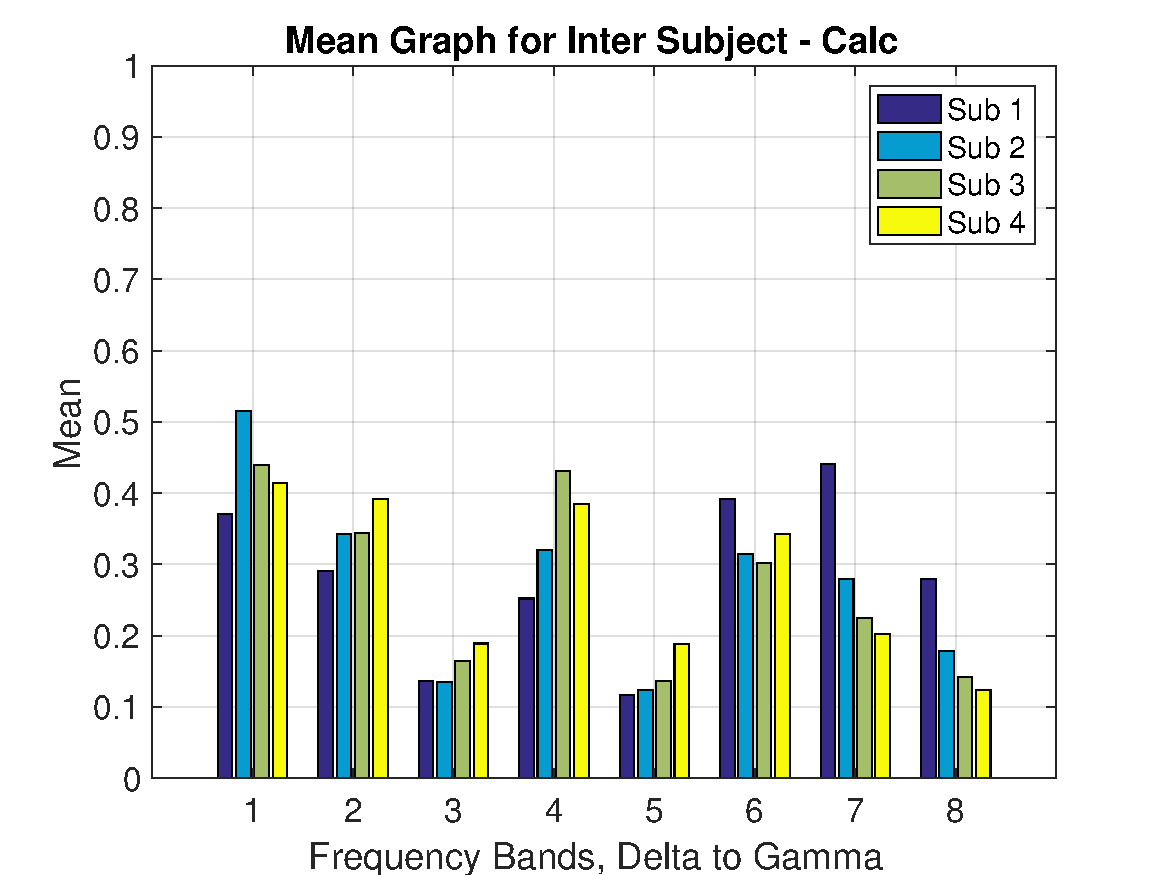
\includegraphics[width=0.9\textwidth]{Chapter-4/1}
    	\caption{Mean of each EEG band for Calculation task}
    	\label{fig:chap41}
    \end{figure}

    \begin{figure}[hbtp]
    	\centering
    	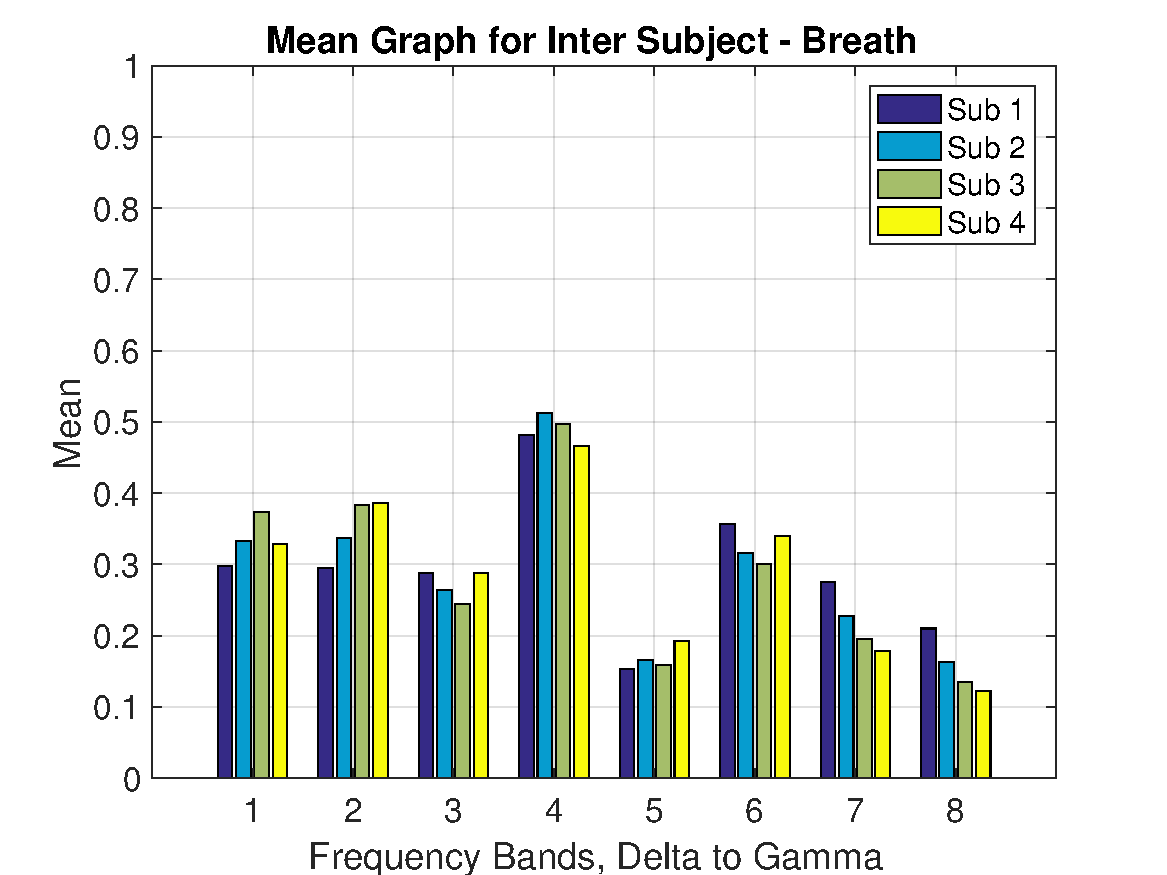
\includegraphics[width=0.9\textwidth]{Chapter-4/3}
    	\caption{Mean of each EEG band for Breathing task}
    	\label{fig:chap43}
    \end{figure}

    \begin{figure}[hbtp]
    	\centering
    	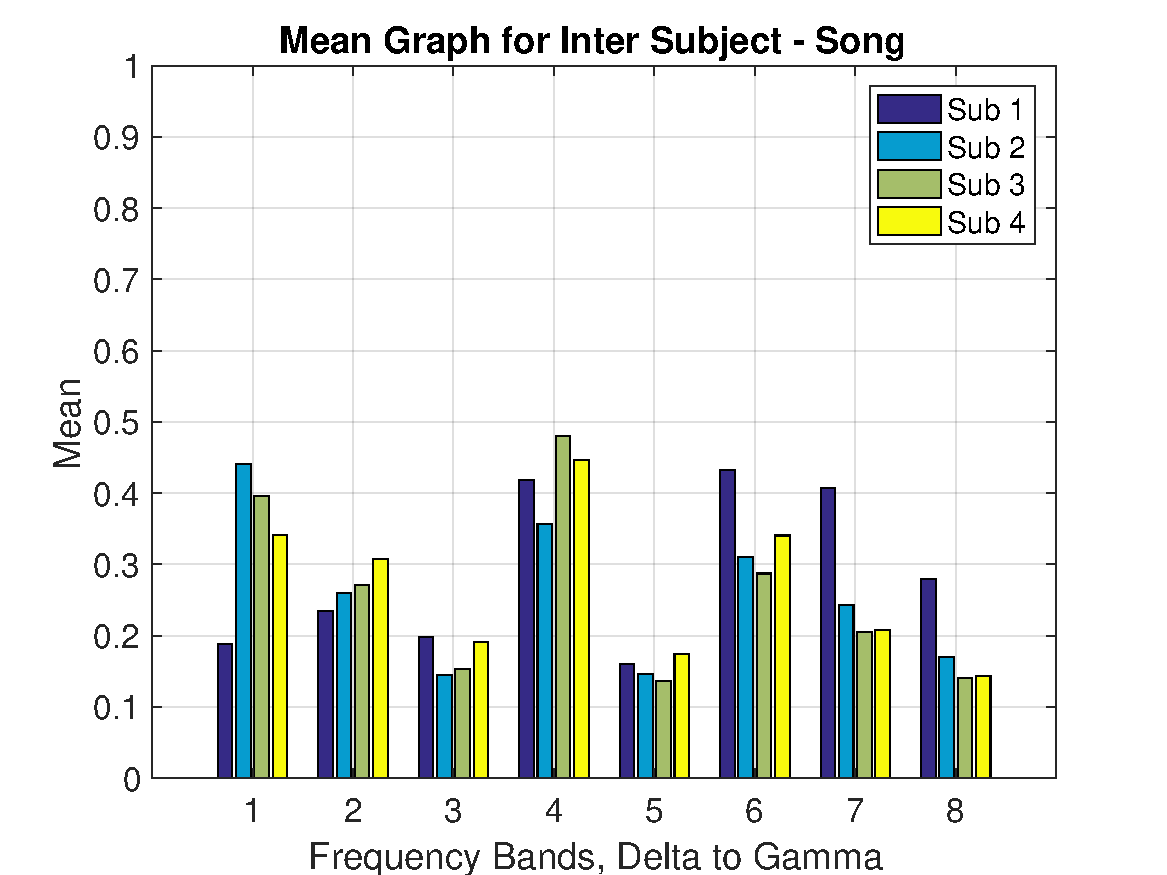
\includegraphics[width=0.9\textwidth]{Chapter-4/5}
    	\caption{Mean of each EEG band for Singing task}
    	\label{fig:chap45}
    \end{figure}

    \begin{figure}[hbtp]
    	\centering
    	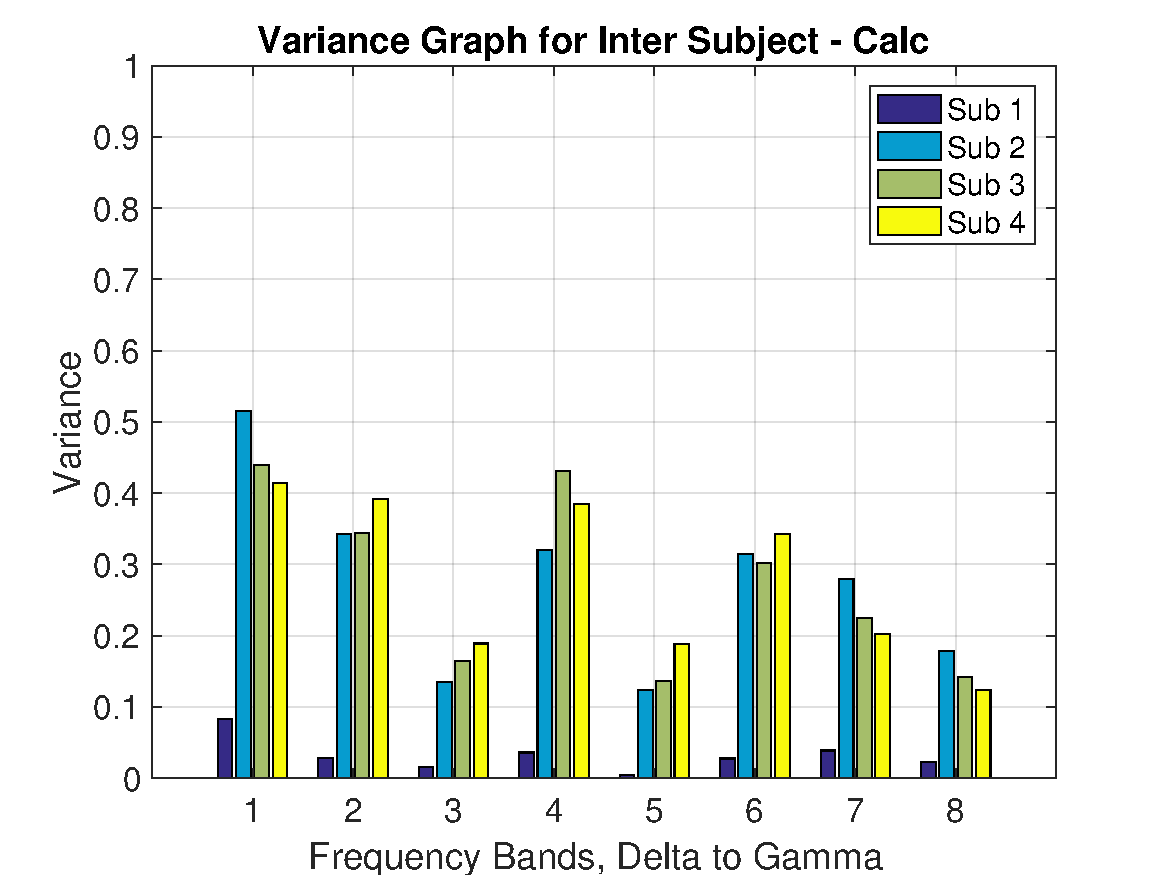
\includegraphics[width=0.9\textwidth]{Chapter-4/2}
    	\caption{Variance of each EEG band for Calculation task}
    	\label{fig:chap42}
    \end{figure}

    \begin{figure}[hbtp]
    	\centering
    	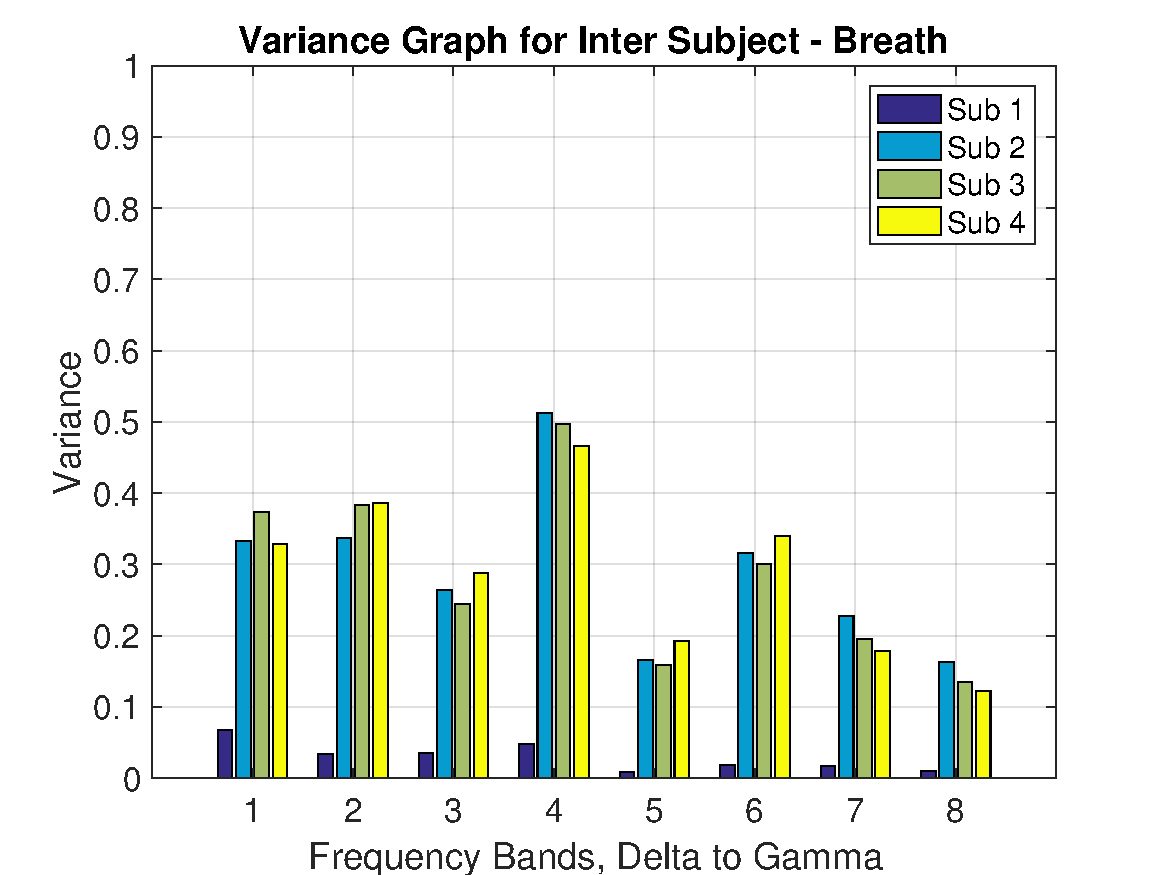
\includegraphics[width=0.9\textwidth]{Chapter-4/4}
    	\caption{Variance of each EEG band for Breathing task}
    	\label{fig:chap44}
    \end{figure}

    \begin{figure}[hbtp]
    	\centering
    	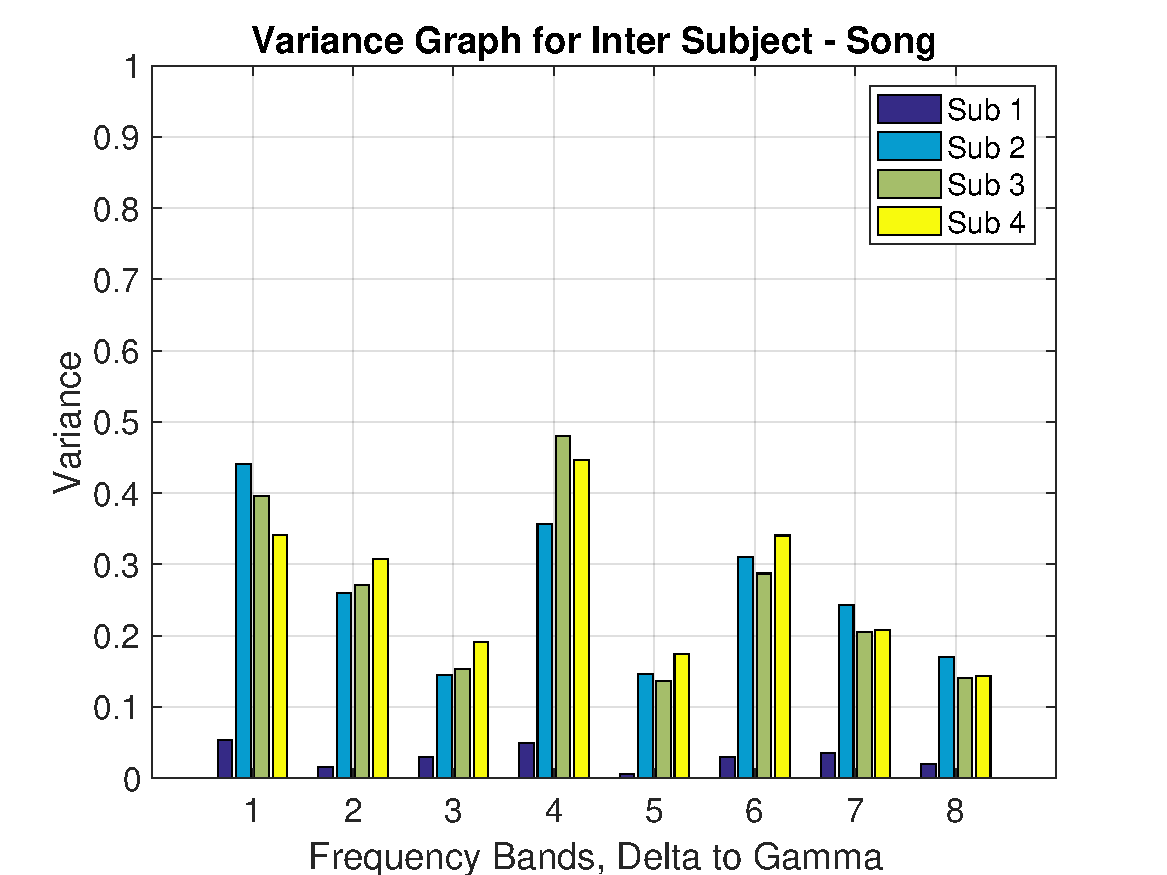
\includegraphics[width=0.9\textwidth]{Chapter-4/6}
    	\caption{Variance of each EEG band for Singing task}
    	\label{fig:chap46}
    \end{figure}

    \FloatBarrier

    \section{Classifier Performance}
    Performance of the Mahalanobis Distance classifier, the Neural Network classifier and the SVM classifier are discussed in this section. As discussed in Section \ref{Chap3:Classifiers}, we consider two types of EEG data classification. First is to identify the ``task'' performed by the subject. We call this ``Intra-subject classification''. Second type of classification is to identify the subject among group of subject performing similar tasks. We call this ``Inter-subject classification''. Here task refers to the brain activity like doing mathematical calculation, concentrating on breathing or mentally singing a song(refer Table \ref{Tasks} for more details).
    
    We also need to consider comparison of baseline performance verses classifier performance. For example, if the feature vectors of all the classes are uniformly distributed, then, if we randomly choose a class among given classes, the probability of being right is given by Equation \ref{EQ:chap4base}.

    	\begin{equation}
    		P =  \frac{1}{N} \;,
    		\label{EQ:chap4base}
    	\end{equation}

    	\noindent where N is the total number of classes. We call this the ``baseline performance''.

    \subsection{Intra-subject Classification}
    For this experiment, we collected data from four different test subjects performing three different tasks repeated five times each. As discussed in Section \ref{Chap3:Classifiers}, training and testing split was 70\% and 30\% respectively.
    
    \subsubsection{Mahalanobis Distance}
    Table \ref{MICT} and Figure \ref{fig:chap4IntraMT} show the overall accuracy of the Mahalanobis distance classifier for intra-subject classification. Table \ref{MICTPR} and Figure \ref{fig:chap4IntraMTPR} show the TPR for different tasks using the Mahalanobis distance classifier. Also, Table \ref{MICFPR} and Figure \ref{fig:chap4IntraMFPR} show the FPR for different tasks using the Mahalanobis distance classifier.
		\begin{table}[h!]
			\centering
			\caption{Intra-subject Classification using Mahalanobis Distance, Total Accuracy}
			\label{MICT}
			\begin{tabular}{c c c c}
				\hline
				Sub &Min &Max &Average\\\hline
				1 &33.33 &55.56 &44.89\\
				2 &44.44 &66.67 &55.78\\
				3 &35.56 &46.67 &42.67\\
				4 &44.44 &71.11 &61.56\\
			\end{tabular}
		\end{table}
        
        \begin{figure}[hbtp]
	    	\centering
	    	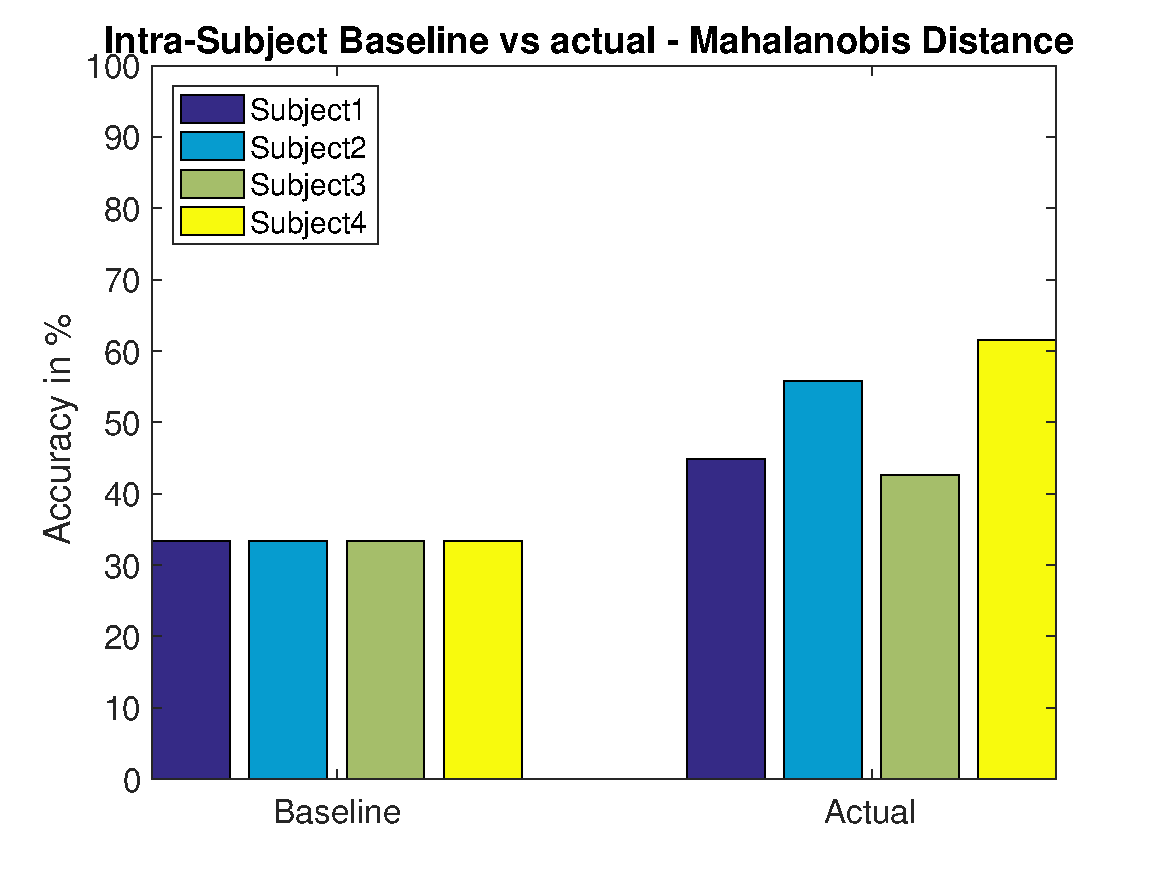
\includegraphics[width=0.90\textwidth]{Chapter-4/base_tm}
	    	\caption{Total accuracy for Intra-subject classification using the Mahalanobis Distance Classifier}
	    	\label{fig:chap4IntraMT}
    	\end{figure}

    	\begin{figure}[hbtp]
	    	\centering
	    	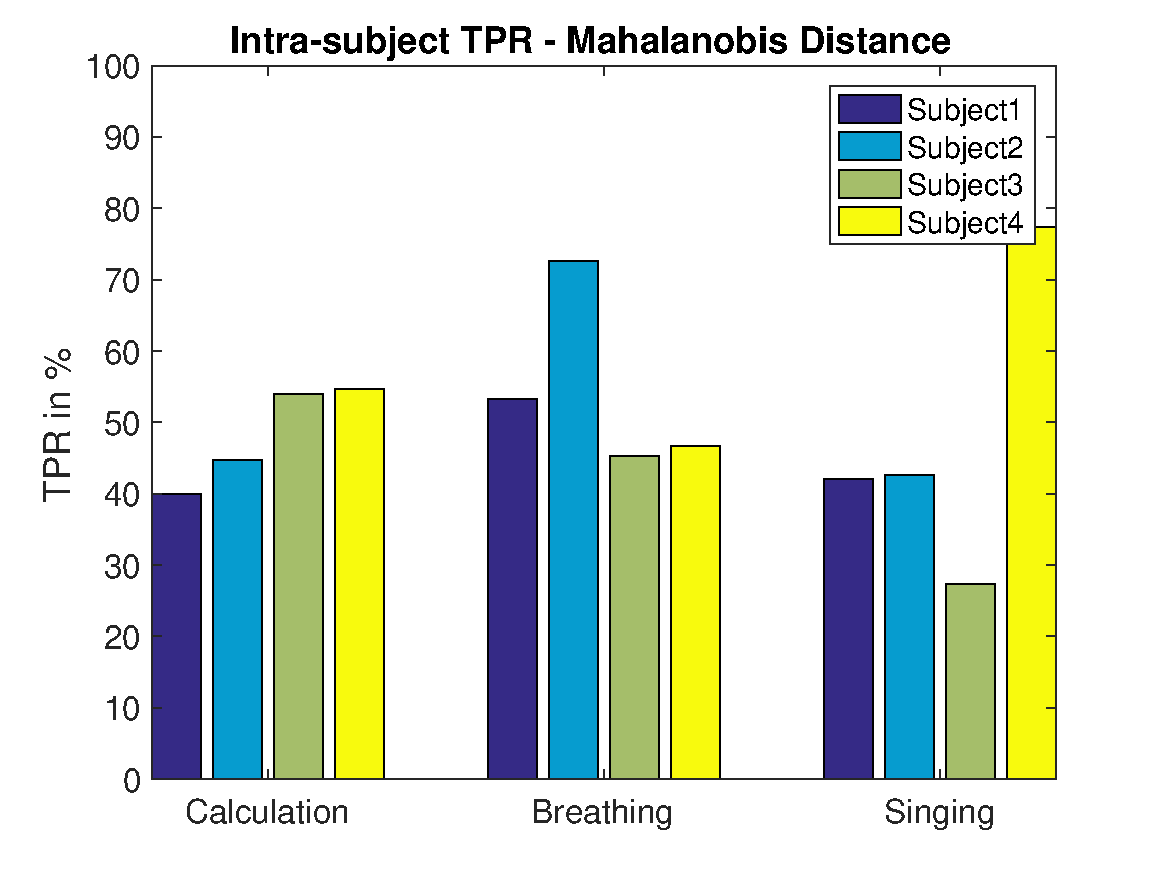
\includegraphics[width=0.90\textwidth]{Chapter-4/base_tprm}
	    	\caption{TPR for Intra-subject classification using the Mahalanobis Distance Classifier}
	    	\label{fig:chap4IntraMTPR}
    	\end{figure}

    	\begin{figure}[hbtp]
	    	\centering
	    	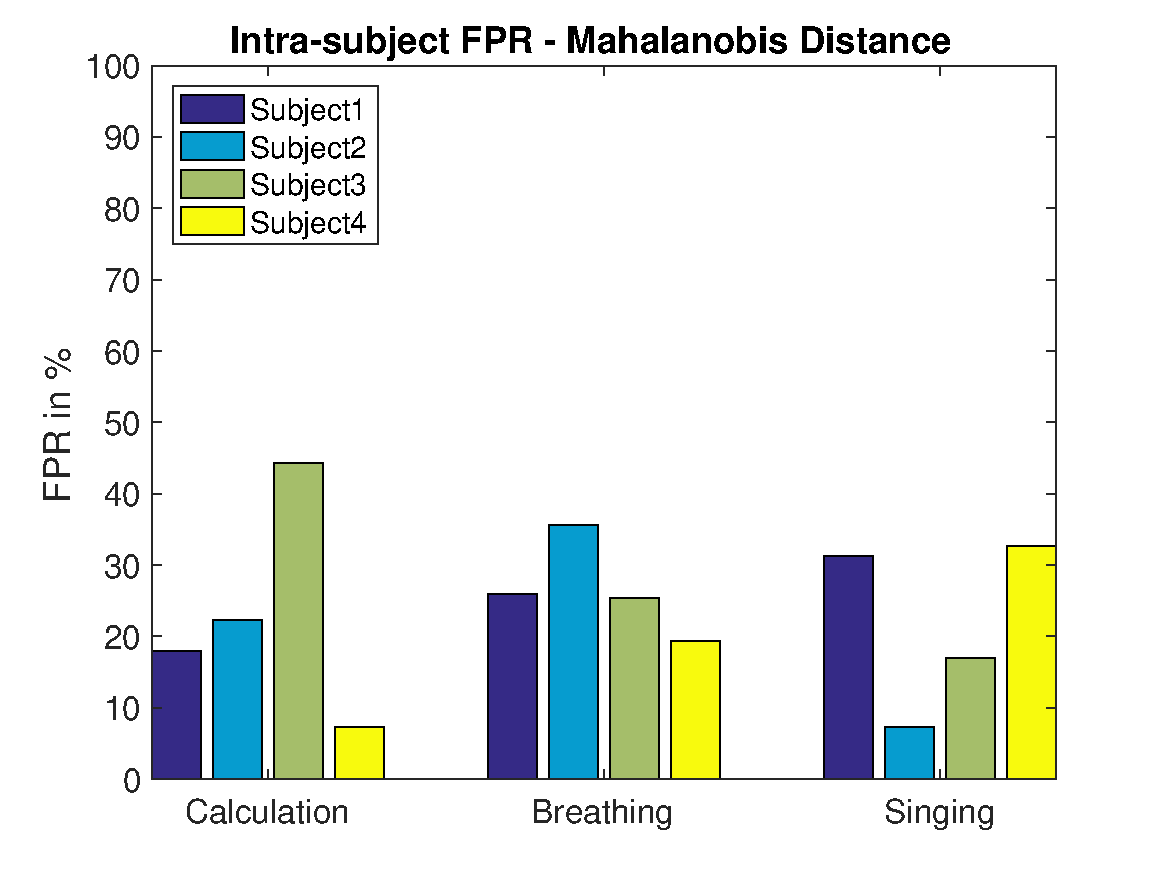
\includegraphics[width=0.90\textwidth]{Chapter-4/base_fprm}
	    	\caption{FPR for Intra-subject classification using the Mahalanobis Distance Classifier}
	    	\label{fig:chap4IntraMFPR}
    	\end{figure}

		\begin{table}[h!]
			\centering
			\caption{Intra-subject Classification using Mahalanobis Distance, TPR for Calculation, Breathing and Singing Task}
			\label{MICTPR}
			\subfloat[Calculation]{
			\begin{tabular}{c c c c}
				\hline
				Sub &Min &Max &Average\\\hline
				1 &20.00 &66.67 &40.00\\
				2 &26.67 &73.33 &44.67\\
				3 &20.00 &80.00 &54.00\\
				4 &33.33 &73.33 &54.67\\
			\end{tabular}
			}\hfill
			\subfloat[Breathing]{
			\begin{tabular}{c c c c}
				\hline
				Sub &Min &Max &Average\\\hline
				1 &40.00 &73.33 &53.33\\
				2 &60.00 &86.67 &72.67\\
				3 &26.67 &73.33 &45.33\\
				4 &20.00 &73.33 &46.67\\
			\end{tabular}
			}\\
			\subfloat[Singing]{
			\begin{tabular}{c c c c}
				\hline
				Sub &Min &Max &Average\\\hline
				1 &13.33 &66.67 &42.00\\
				2 &26.67 &73.33 &42.67\\
				3 &13.33 &66.67 &27.33\\
				4 &60.00 &93.33 &77.33\\
			\end{tabular}
			}
		\end{table}	

		\begin{table}[h!]
			\centering
			\caption{Intra-subject Classification using Mahalanobis Distance, FPR for Calculation, Breathing and Singing Task}
			\label{MICFPR}
			\subfloat[Calculation]{
			\begin{tabular}{c c c c}
				\hline
				Sub &Min &Max &Average\\\hline
				1 &3.33 &36.67  &18.00\\
				2 &13.33 &40.00 &22.33\\
				3 &33.33 &60.00 &44.33\\
				4 &0.00 &16.67  &7.33\\
			\end{tabular}
			}\hfill
			\subfloat[Breathing]{
			\begin{tabular}{c c c c}
				\hline
				Sub &Min &Max &Average\\\hline
				1 &20.00 &36.67 &26.00\\
				2 &23.33 &53.33 &35.67\\
				3 &6.67 &43.33  &25.33\\
				4 &3.33 &36.67  &19.33\\
			\end{tabular}
			}\\
			\subfloat[Singing]{
			\begin{tabular}{c c c c}
				\hline
				Sub &Min &Max &Average\\\hline
				1 &10.00 &46.67 &31.33\\
				2 &0.00 &13.33  &7.33\\
				3 &6.67 &23.33  &17.00\\
				4 &20.00 &53.33 &32.67\\
			\end{tabular}
			}
		\end{table}

        \FloatBarrier
    \subsubsection{Neural Networks}
    Table \ref{NICT} and Figure \ref{fig:chap4IntraNT} show the overall accuracy of the Neural Networks classifier for intra-subject classification. Table \ref{NICTPR} and Figure \ref{fig:chap4IntraNTPR} show the TPR for different tasks using the Neural Networks classifier. Also, Table \ref{NICFPR} and Figure \ref{fig:chap4IntraNFPR} show the FPR for different tasks using the Neural Networks classifier.
    
		\begin{table}[h!]
			\centering
			\caption{Intra-subject Classification using Neural Networks, Total Accuracy}
			\label{NICT}
			\begin{tabular}{c c c c}
				\hline
				Sub &Min &Max &Average\\\hline
				1 &53.33 &64.44 &58.22\\
				2 &57.78 &73.33 &65.11\\
				3 &44.44 &55.56 &48.44\\
				4 &62.22 &73.00 &66.67\\
			\end{tabular}
		\end{table}
        
        \begin{figure}[hbtp]
	    	\centering
	    	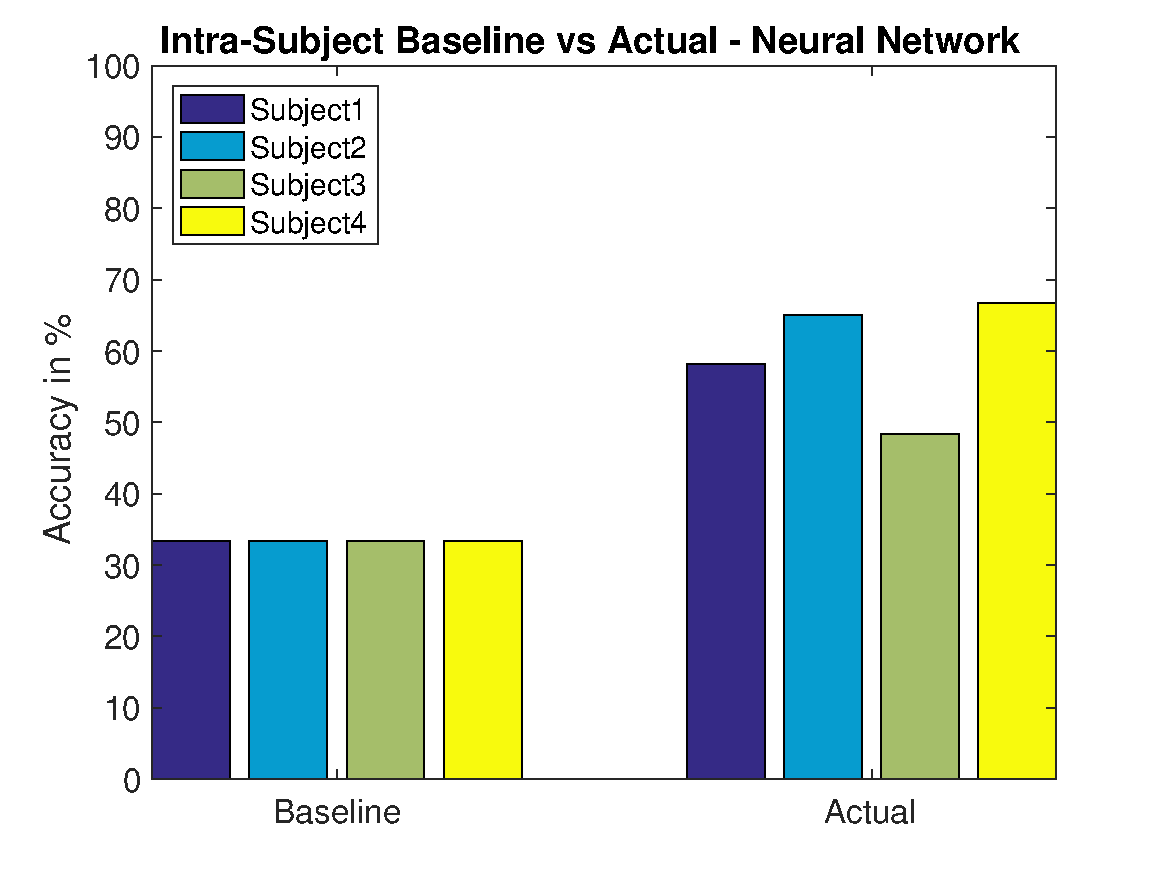
\includegraphics[width=0.90\textwidth]{Chapter-4/base_tn}
	    	\caption{Total accuracy for Intra-subject classification using the Neural Network Classifier}
	    	\label{fig:chap4IntraNT}
    	\end{figure}

    	\begin{figure}[hbtp]
	    	\centering
	    	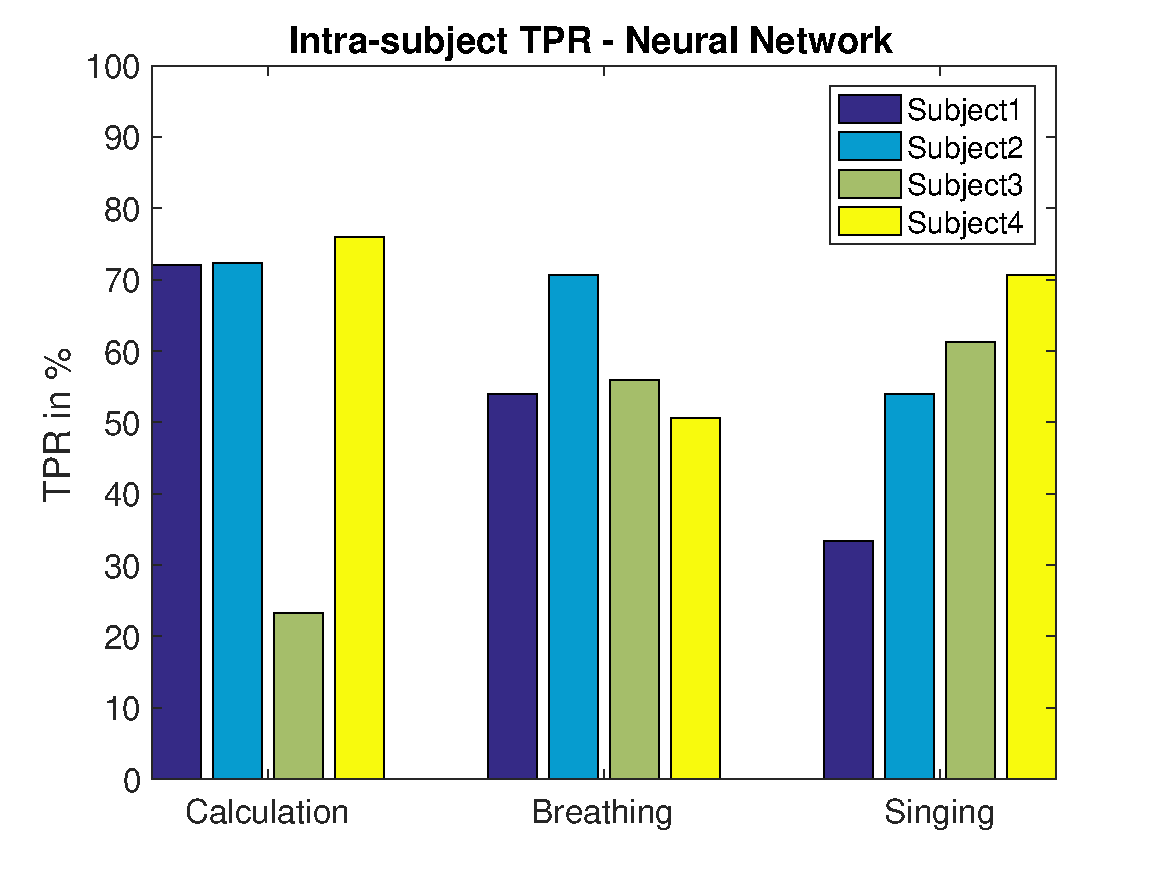
\includegraphics[width=0.90\textwidth]{Chapter-4/base_tprn}
	    	\caption{TPR for Intra-subject classification using the Neural Network Classifier}
	    	\label{fig:chap4IntraNTPR}
    	\end{figure}

    	\begin{figure}[hbtp]
	    	\centering
	    	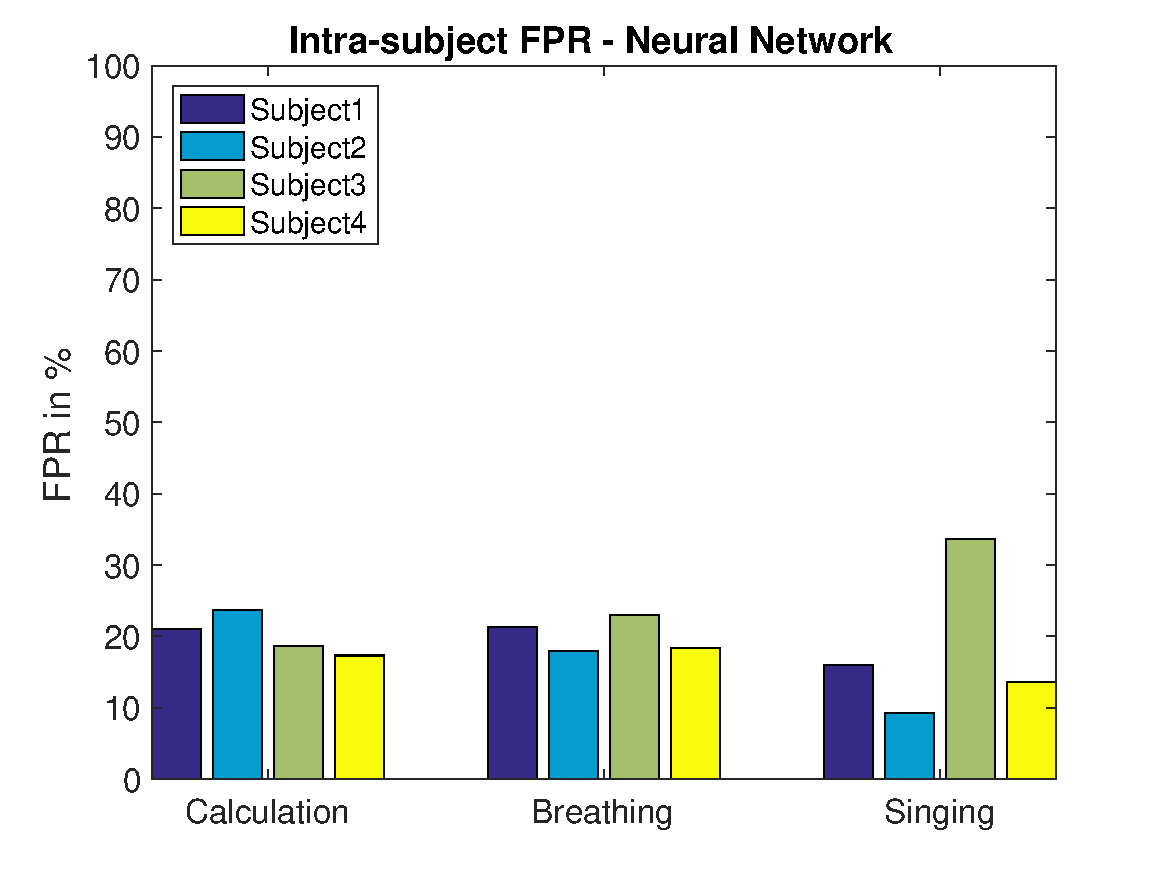
\includegraphics[width=0.90\textwidth]{Chapter-4/base_fprn}
	    	\caption{FPR for Intra-subject classification using the Neural Network Classifier}
	    	\label{fig:chap4IntraNFPR}
    	\end{figure}


		\begin{table}[h!]
			\centering
			\caption{Intra-subject Classification using Neural Networks, TPR for Calculation, Breathing and Singing Task}
			\label{NICTPR}
			\subfloat[Calculation]{
			\begin{tabular}{c c c c}
				\hline
				Sub &Min &Max &Average\\\hline
				1 &60.00 &86.67 &72.00\\
				2 &46.67 &93.33 &72.33\\
				3 &6.67 &33.33  &23.33\\
				4 &66.67 &93.33 &76.00\\
			\end{tabular}
			}\hfill
			\subfloat[Breathing]{
			\begin{tabular}{c c c c}
				\hline
				Sub &Min &Max &Average\\\hline
				1 &33.33 &66.67 &54.00\\
				2 &66.67 &86.67 &70.67\\
				3 &26.67 &66.67 &56.00\\
				4 &33.33 &66.67 &50.67\\
			\end{tabular}
			}\\
			\subfloat[Singing]{
			\begin{tabular}{c c c c}
				\hline
				Sub &Min &Max &Average\\\hline
				1 &13.33 &53.33 &33.33\\
				2 &26.67 &80.00 &54.00\\
				3 &40.00 &86.67 &61.33\\
				4 &60.00 &93.33 &70.67\\
			\end{tabular}
			}
		\end{table}

		\begin{table}[h!]
			\centering
			\caption{Intra-subject Classification using Neural Networks, FPR for Calculation, Breathing and Singing Task}
			\label{NICFPR}
			\subfloat[Calculation]{
			\begin{tabular}{c c c c}
				\hline
				Sub &Min &Max &Average\\\hline
				1 &13.33 &36.67 &21.00\\
				2 &16.67 &30.00 &23.67\\
				3 &13.33 &33.33 &18.67\\
				4 &10.00 &33.33 &17.33\\
			\end{tabular}
			}\hfill
			\subfloat[Breathing]{
			\begin{tabular}{c c c c}
				\hline
				Sub &Min &Max &Average\\\hline
				1 &10.00 &33.33 &21.33\\
				2 &3.33 &26.67  &18.00\\
				3 &10.00 &36.67 &23.00\\
				4 &6.67 &26.67  &18.33\\
			\end{tabular}
			}\\
			\subfloat[Singing]{
			\begin{tabular}{c c c c}
				\hline
				Sub &Min &Max &Average\\\hline
				1 &10.00 &23.33 &16.00\\
				2 &3.33 &13.33  &9.33\\
				3 &20.00 &60.00 &33.67\\
				4 &3.33 &23.33  &13.67\\
			\end{tabular}
			}			
		\end{table}
		\FloatBarrier
    \subsubsection{Support Vector Machines}
    Table \ref{SICT} and Figure \ref{fig:chap4IntraST} show the overall accuracy of the SVM classifier for intra-subject classification. Table \ref{SICTPR} and Figure \ref{fig:chap4IntraSTPR} show the TPR for different tasks using the SVM classifier. Also, Table \ref{SICFPR} and Figure \ref{fig:chap4IntraSFPR} show the FPR for different tasks using the SVM classifier.
		\begin{table}[h!]
			\centering
			\caption{Intra-subject Classification using Support Vector Machines, Total Accuracy}
			\label{SICT}
			\begin{tabular}{c c c c}
				\hline
				Sub &Min &Max &Average\\\hline
				1 &40.00 &57.78 &50.67\\
				2 &55.56 &71.11 &66.44\\
				3 &33.33 &48.89 &41.11\\
				4 &57.78 &73.33 &65.56\\
			\end{tabular}
		\end{table}

		\begin{figure}[hbtp]
	    	\centering
	    	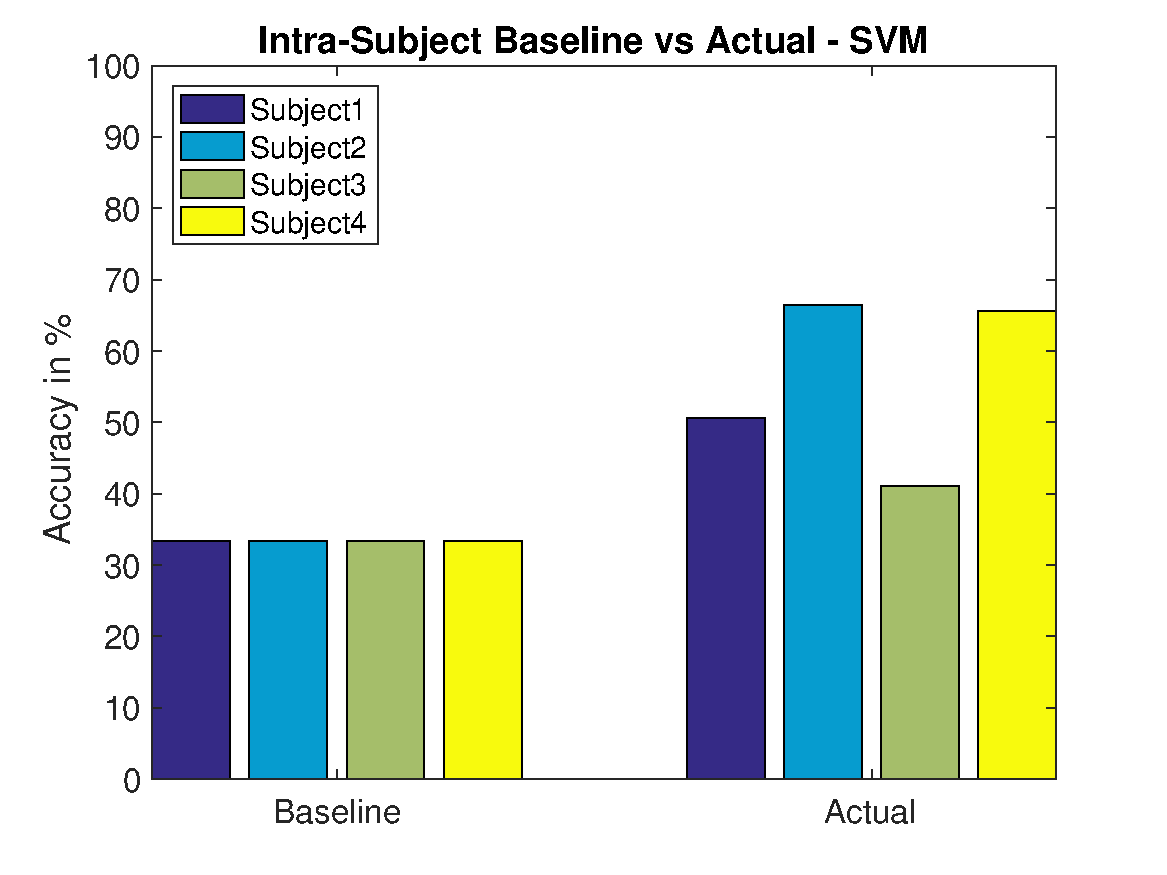
\includegraphics[width=0.90\textwidth]{Chapter-4/base_ts}
	    	\caption{Total accuracy for Intra-subject classification using the SVM Classifier}
	    	\label{fig:chap4IntraST}
    	\end{figure}

    	\begin{figure}[hbtp]
	    	\centering
	    	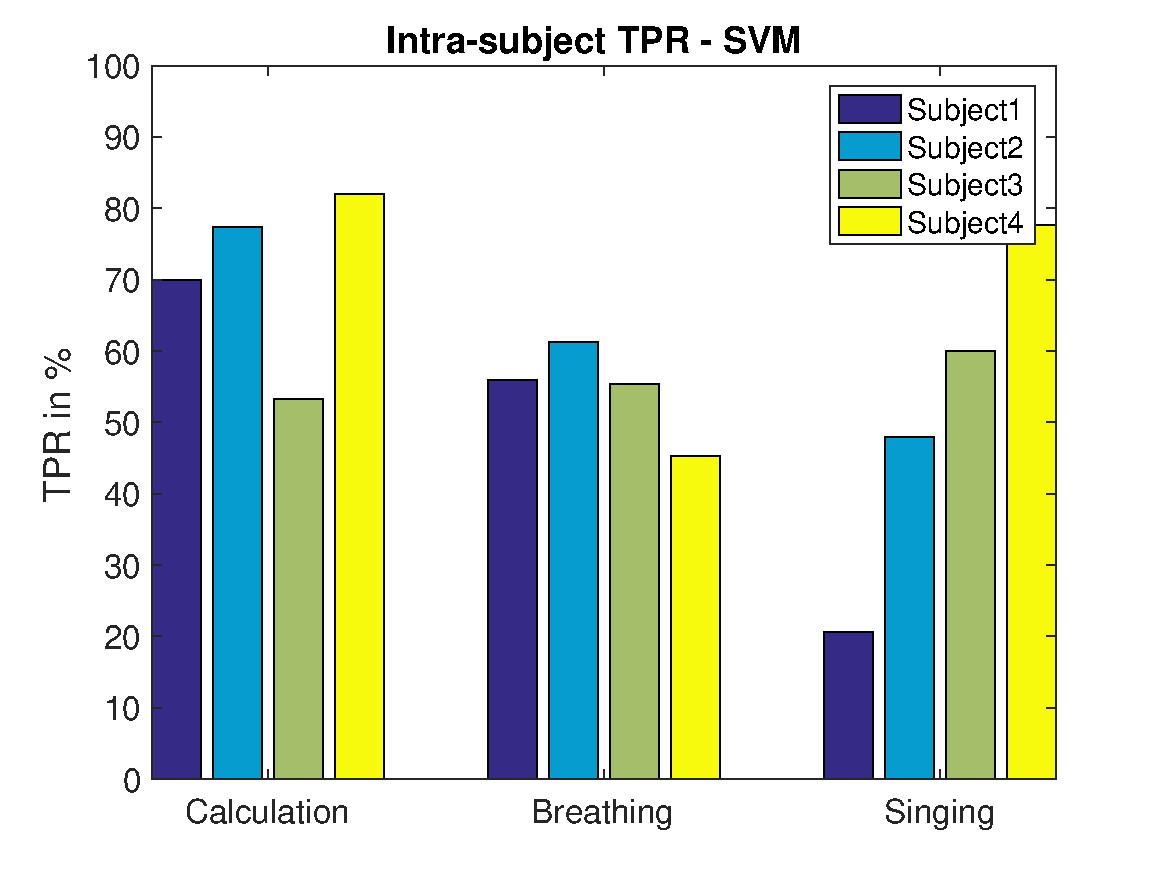
\includegraphics[width=0.9\textwidth]{Chapter-4/base_tprs}
	    	\caption{TPR for Intra-subject classification using the SVM Classifier}
	    	\label{fig:chap4IntraSTPR}
    	\end{figure}

    	\begin{figure}[hbtp]
	    	\centering
	    	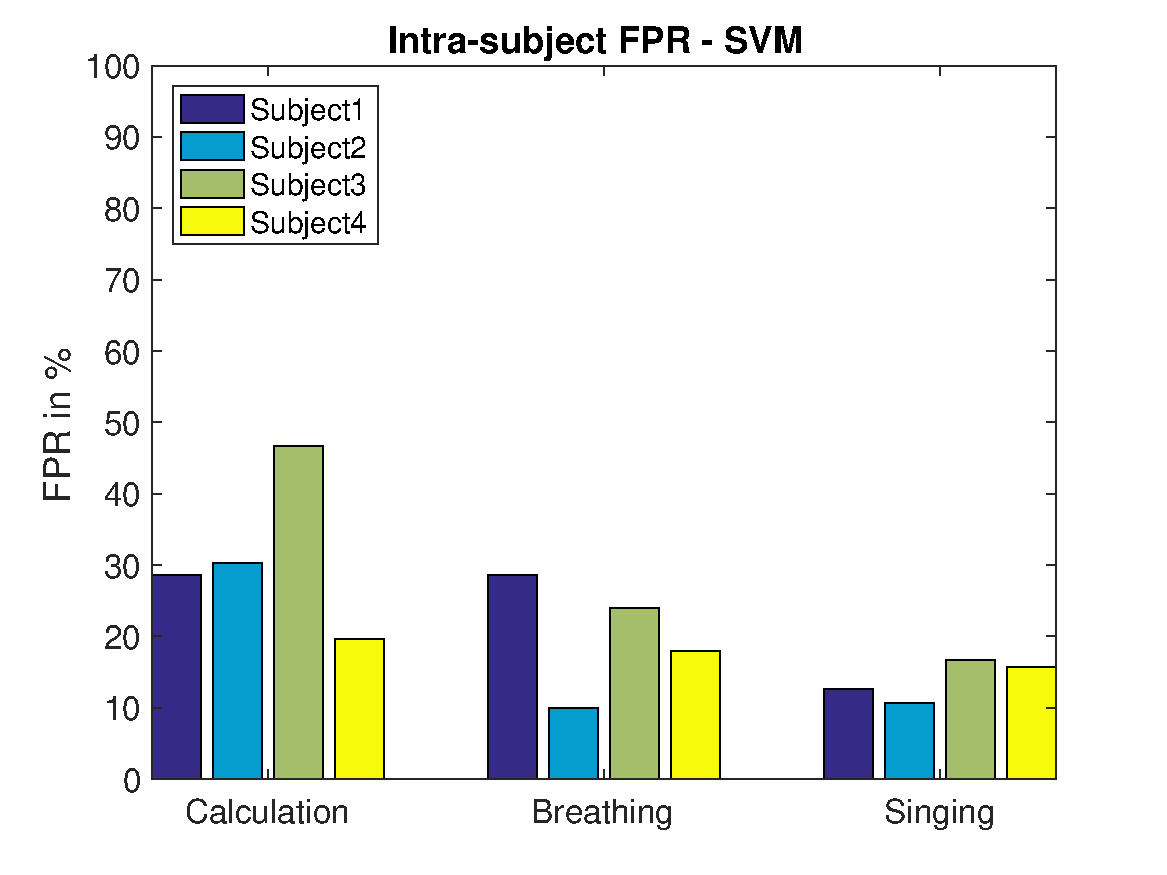
\includegraphics[width=0.90\textwidth]{Chapter-4/base_fprs}
	    	\caption{FPR for Intra-subject classification using the SVM Classifier}
	    	\label{fig:chap4IntraSFPR}
    	\end{figure}

		\begin{table}[h!]
			\centering
			\caption{Intra-subject Classification using Support Vector Machines, TPR for Calculation, Breathing and Singing Task}
			\label{SICTPR}
			\subfloat[Calculation]{
			\begin{tabular}{c c c c}
				\hline
				Sub &Min &Max &Average\\\hline
				1 &53.33 &86.67 &70.00\\
				2 &60.00 &93.33 &77.33\\
				3 &40.00 &73.33 &53.33\\
				4 &73.33 &93.33 &82.00\\
			\end{tabular}
			}\hfill
			\subfloat[Breathing]{
			\begin{tabular}{c c c c}
				\hline
				Sub &Min &Max &Average\\\hline
				1 &40.00 &73.33 &56.00\\
				2 &33.33 &73.33 &61.33\\
				3 &40.00 &73.33 &55.33\\
				4 &40.00 &66.67 &45.33\\
			\end{tabular}
			}\\
			\subfloat[Singing]{
			\begin{tabular}{c c c c}
				\hline
				Sub &Min &Max &Average\\\hline
				1 &6.67 &40.00  &20.67\\
				2 &33.33 &66.67 &48.00\\
				4 &46.67 &73.33 &60.00\\
				4 &68.67 &77.00 &77.67\\
			\end{tabular}
			}
		\end{table}

		\begin{table}[h!]
			\centering
			\caption{Intra-subject Classification using Support Vector Machines, FPR for Calculation, Breathing and Singing Task}
			\label{SICFPR}
			\subfloat[Calculation]{
			\begin{tabular}{c c c c}
				\hline
				Sub &Min &Max &Average\\\hline
				1 &20.00 &36.67 &28.67\\
				2 &23.33 &40.00 &30.33\\
				3 &36.67 &60.00 &46.67\\
				4 &10.00 &33.33 &19.67\\
			\end{tabular}
			}\hfill
			\subfloat[Breathing]{
			\begin{tabular}{c c c c}
				\hline
				Sub &Min &Max &Average\\\hline
				1 &16.67 &60.00 &28.67\\
				2 &0.00 &20.00  &10.00\\
				3 &13.33 &40.00 &24.00\\
				4 &6.67 &40.00  &18.00\\
			\end{tabular}
			}\\
			\subfloat[Singing]{
			\begin{tabular}{c c c c}
				\hline
				Sub &Min &Max &Average\\\hline
				1 &3.33 &26.67 &12.67\\
				2 &3.33 &20.00 &10.67\\
				3 &6.67 &33.33 &16.67\\
				4 &0.00 &23.33 &15.67\\
			\end{tabular}
			}
		\end{table}
		\FloatBarrier

	\subsection{Inter-Subject Classification}
    For this experiment, we collected data from four different test subjects performing three different tasks repeated five times each. As discussed in Section \ref{Chap3:Classifiers}, training and testing split was 70\% and 30\% respectively.
    \subsubsection{Mahalanobis Distance}
    Table \ref{InMD} and Figure \ref{fig:chap4InterMT} show the overall accuracy of the Mahalanobis distance classifier for inter-subject classification. Table \ref{InMDTPR} and Figure \ref{fig:chap4InterMTPR} show the TPR for different test subjects using the Mahalanobis distance classifier. Also, Table \ref{InMDFPR} and Figure \ref{fig:chap4InterMFPR} show the FPR for different test subjects using the Mahalanobis distance classifier.
		\begin{table}[h!]
			\centering
			\caption{Inter-subject Classification for 4 subjects using Mahalanobis Distance - Total Accuracy}
			\label{InMD}
			\begin{tabular}{l c c c}
				\hline
				Task &Min &Max &Average\\\hline
				Calculation &65.00 &85.00 &75.50\\
				Breathing &50.00 &65.00   &57.67\\
				Singing &55.00 &78.33     &69.00\\
			\end{tabular}
		\end{table}

		\begin{figure}[hbtp]
	    	\centering
	    	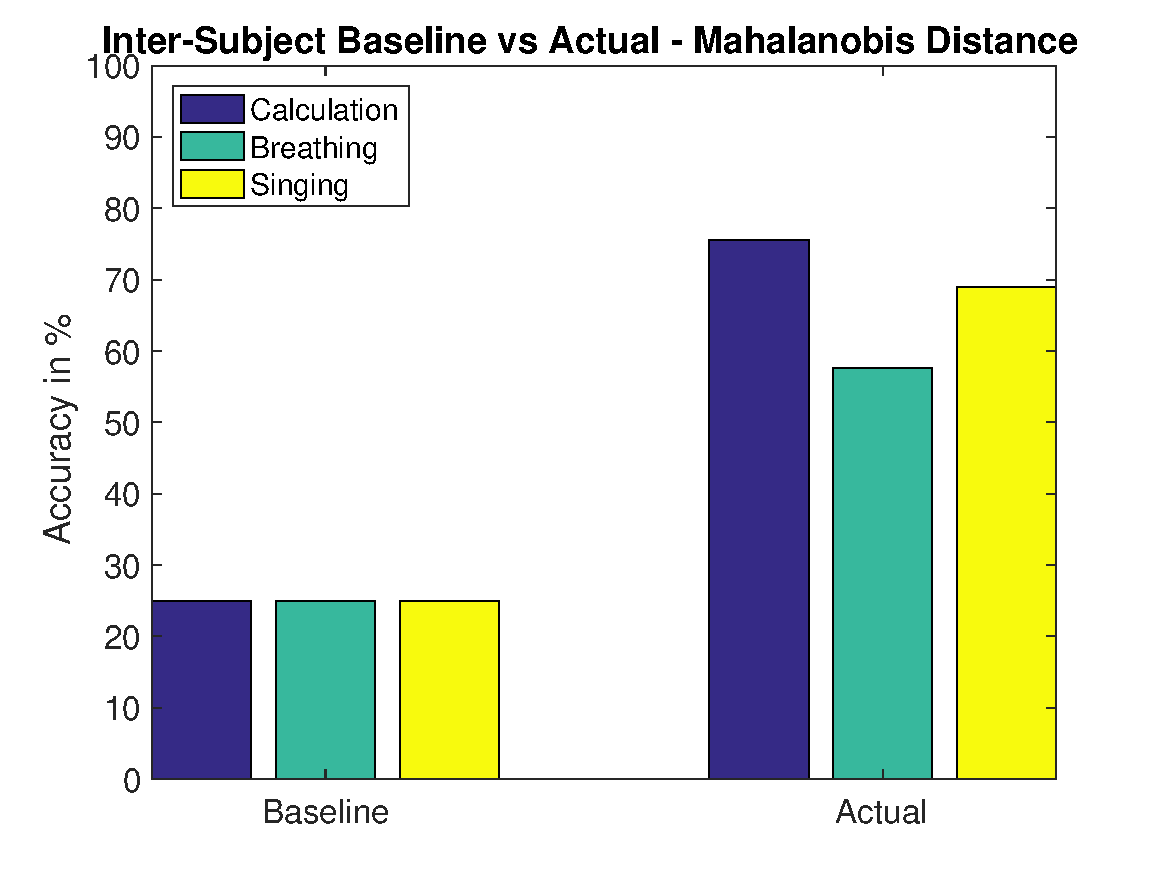
\includegraphics[width=0.90\textwidth]{Chapter-4/base_tim}
	    	\caption{Total accuracy for Inter-subject classification using the Mahalanobis Distance Classifier}
	    	\label{fig:chap4InterMT}
    	\end{figure}

    	\begin{figure}[hbtp]
	    	\centering
	    	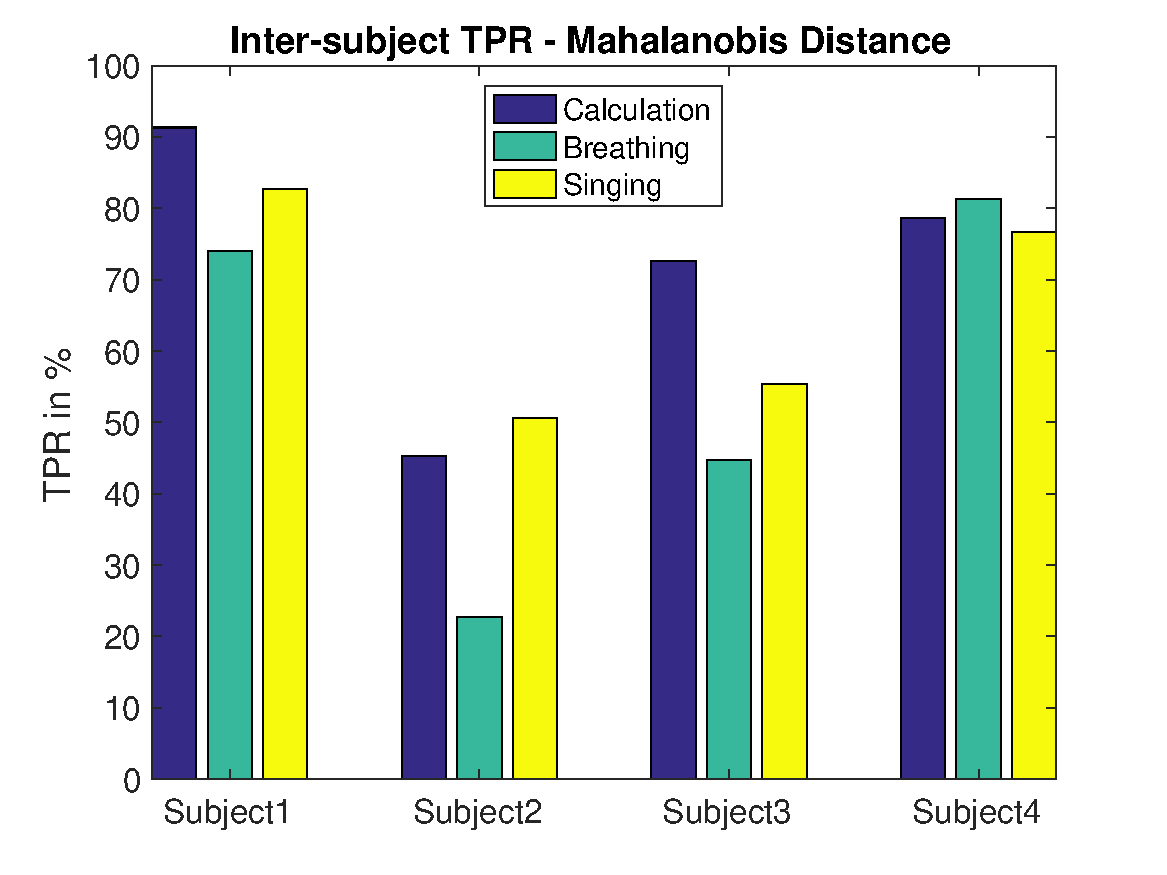
\includegraphics[width=0.90\textwidth]{Chapter-4/base_tprim}
	    	\caption{TPR for Inter-subject classification using the Mahalanobis Distance Classifier}
	    	\label{fig:chap4InterMTPR}
    	\end{figure}

    	\begin{figure}[hbtp]
	    	\centering
	    	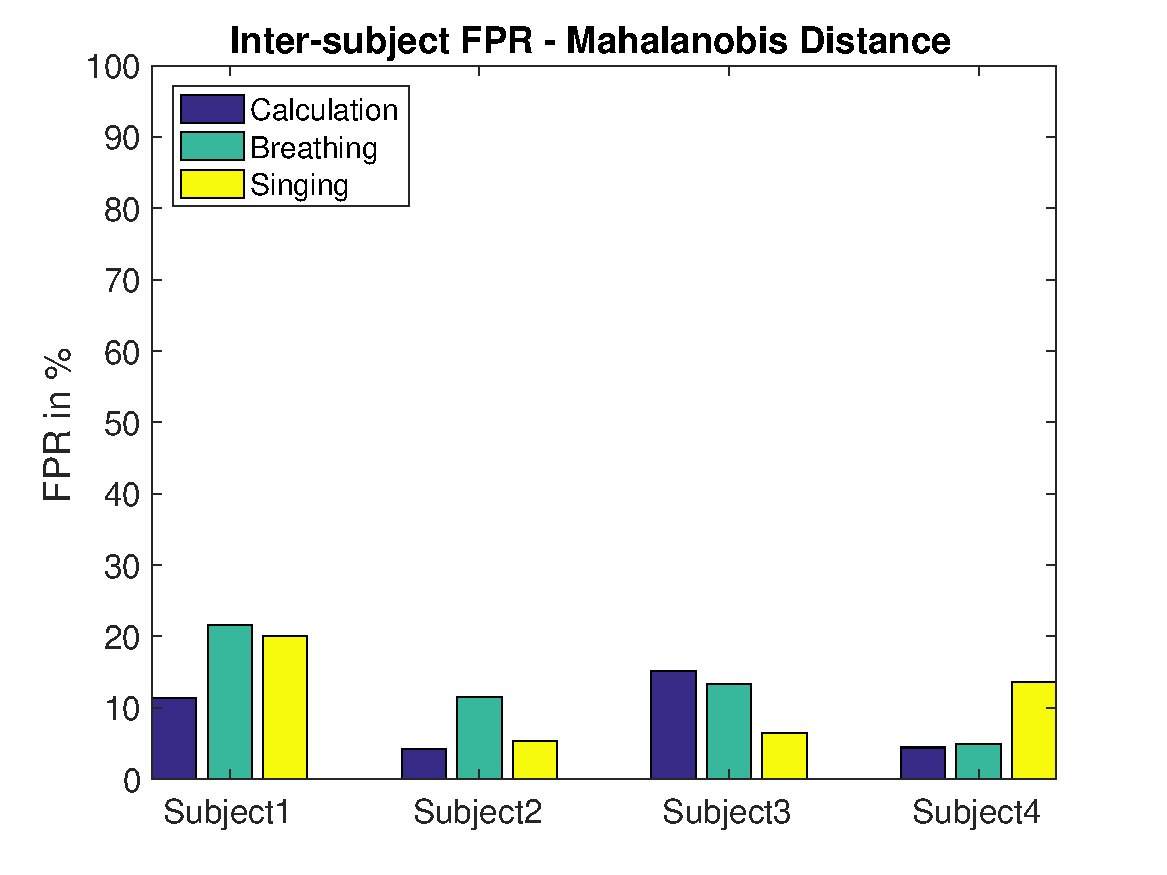
\includegraphics[width=0.90\textwidth]{Chapter-4/base_fprim}
	    	\caption{FPR for Inter-subject classification using the Mahalanobis Distance Classifier}
	    	\label{fig:chap4InterMFPR}
    	\end{figure}

		\begin{table}[h!]
			\centering
			\caption{Inter-subject Classification for 4 subjects using Mahalanobis Distance - TPR for Subject 1-4}
			\label{InMDTPR}
			\subfloat[Subject 1]{
			\begin{tabular}{l c c c}
				\hline
				Task &Min &Max &Average\\\hline
				Calculation &80.00 &100.00 &91.33\\
				Breathing &60.00 &93.33    &74.00\\
				Singing &73.33 &100.00     &82.67\\
			\end{tabular}
			}\hfill
			\subfloat[Subject 2]{
			\begin{tabular}{l c c c}
				\hline
				Task &Min &Max &Average\\\hline
				Calculation &20.00 &66.67 &45.33\\
				Breathing &6.67 &40.00    &22.67\\
				Singing &33.33 &73.33     &50.67\\
			\end{tabular}
			}\\		
			\subfloat[Subject 3]{
			\begin{tabular}{l c c c}
				\hline
				Task &Min &Max &Average\\\hline
				Calculation &46.67 &93.33 &72.67\\
				Breathing &26.67 &73.33   &44.67\\
				Singing &33.33 &73.33     &55.33\\
			\end{tabular}
			}\hfill
			\subfloat[Subject 4]{
			\begin{tabular}{l c c c}
				\hline
				Task &Min &Max &Average\\\hline
				Calculation &60.00 &86.67 &78.67\\
				Breathing &66.67 &100.00  &81.33\\
				Singing &46.67 &93.33     &76.67\\
			\end{tabular}
			}
		\end{table}

		\begin{table}[h!]
			\centering
			\caption{Inter-subject Classification for 4 subjects using Mahalanobis Distance - FPR for Subject 1-4}
			\label{InMDFPR}
			\subfloat[Subject 1]{
			\begin{tabular}{l c c c}
				\hline
				Task &Min &Max &Average\\\hline
				Calculation &2.22 &17.78 &11.33\\
				Breathing &13.33 &31.11  &21.56\\
				Singing &6.67 &35.56     &20.00\\
			\end{tabular}
			}\hfill
			\subfloat[Subject 2]{
			\begin{tabular}{l c c c}
				\hline
				Task &Min &Max &Average\\\hline
				Calculation &0.00 &8.89 &4.22\\
				Breathing &4.44 &20.00  &11.56\\
				Singing &2.22 &11.11    &5.33\\
			\end{tabular}
			}\\		
			\subfloat[Subject 3]{
			\begin{tabular}{l c c c}
				\hline
				Task &Min &Max &Average\\\hline
				Calculation &6.67 &22.22 &15.11\\
				Breathing &4.44 &28.89   &13.33\\
				Singing &2.22 &15.56     &6.44\\
			\end{tabular}
			}\hfill
			\subfloat[Subject 4]{
			\begin{tabular}{l c c c}
				\hline
				Task &Min &Max &Average\\\hline
				Calculation &2.22 &6.67 &4.44\\
				Breathing &0.00 &8.89   &4.89\\
				Singing &2.22 &28.89    &13.56\\
			\end{tabular}
			}			
		\end{table}
        
 	Inter subject classification with Mahalanobis distance demonstrate a wide variation of TPR for different test subjects. As you can see, Subject 2 and Subject 3 have lower TPR compared to Subject 3 and 4. Also, FPR for Subject 1 is higher compared to the rest of the subjects.

 	\FloatBarrier
		\subsubsection{Neural Networks}
    Table \ref{InNN} and Figure \ref{fig:chap4InterNT} show the overall accuracy of the Neural Networks classifier for inter-subject classification. Table \ref{InNNTPR} and Figure \ref{fig:chap4InterNTPR} show the TPR for different test subjects using the Neural Networks classifier. Also, Table \ref{InNNFPR} and Figure \ref{fig:chap4InterNFPR} show the FPR for different test subjects using the Neural Networks classifier.
		\begin{table}[h!]
			\centering
			\caption{Inter-subject Classification for 4 subjects using Neural Networks - Total Accuracy}
			\label{InNN}
			\begin{tabular}{l c c c}
				\hline
				Task &Min &Max &Average\\\hline
				Calculation &73.33 &85.00 &80.17\\
				Breathing &55.00 &63.33   &59.33\\
				Singing &66.67 &85.00     &73.17\\
			\end{tabular}
		\end{table}
 		
 		\begin{figure}[hbtp]
	    	\centering
	    	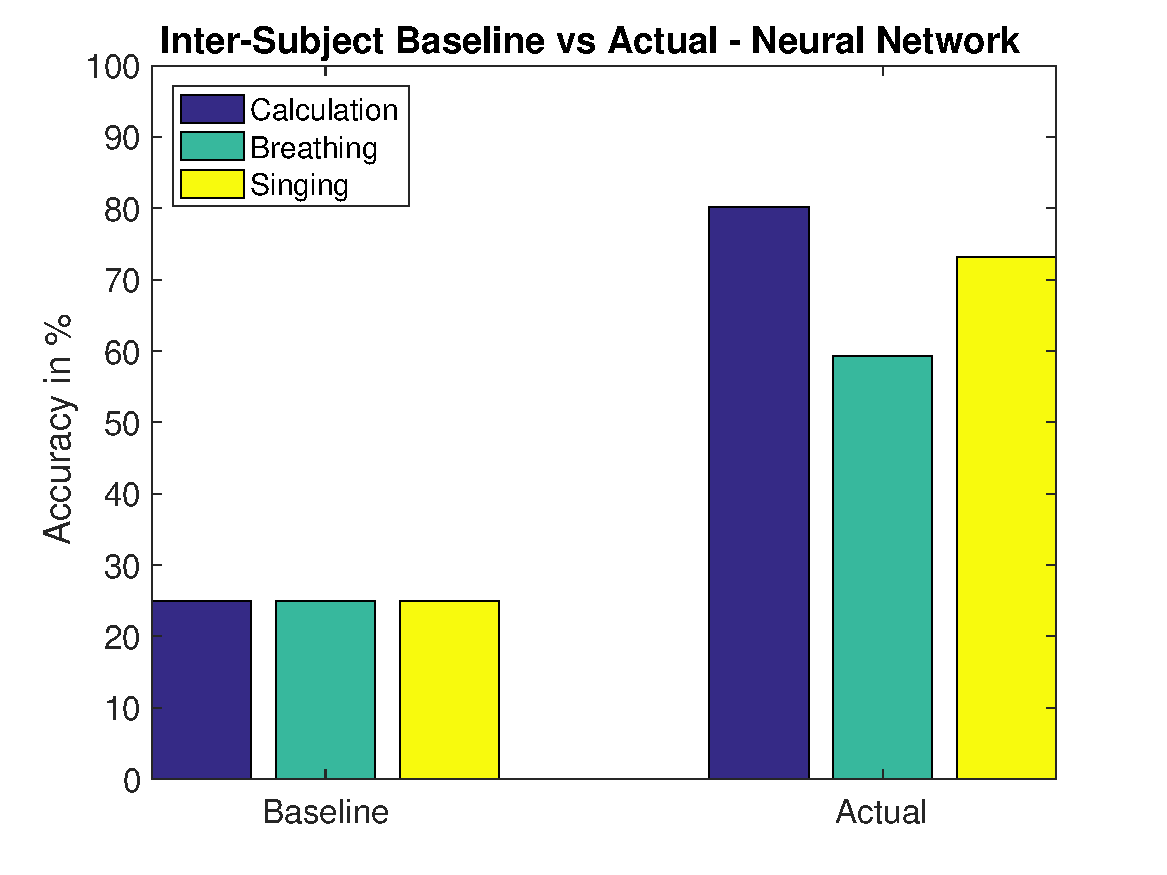
\includegraphics[width=0.90\textwidth]{Chapter-4/base_tin}
	    	\caption{Total accuracy for Inter-subject classification using Neural Networks}
	    	\label{fig:chap4InterNT}
    	\end{figure}

    	\begin{figure}[hbtp]
	    	\centering
	    	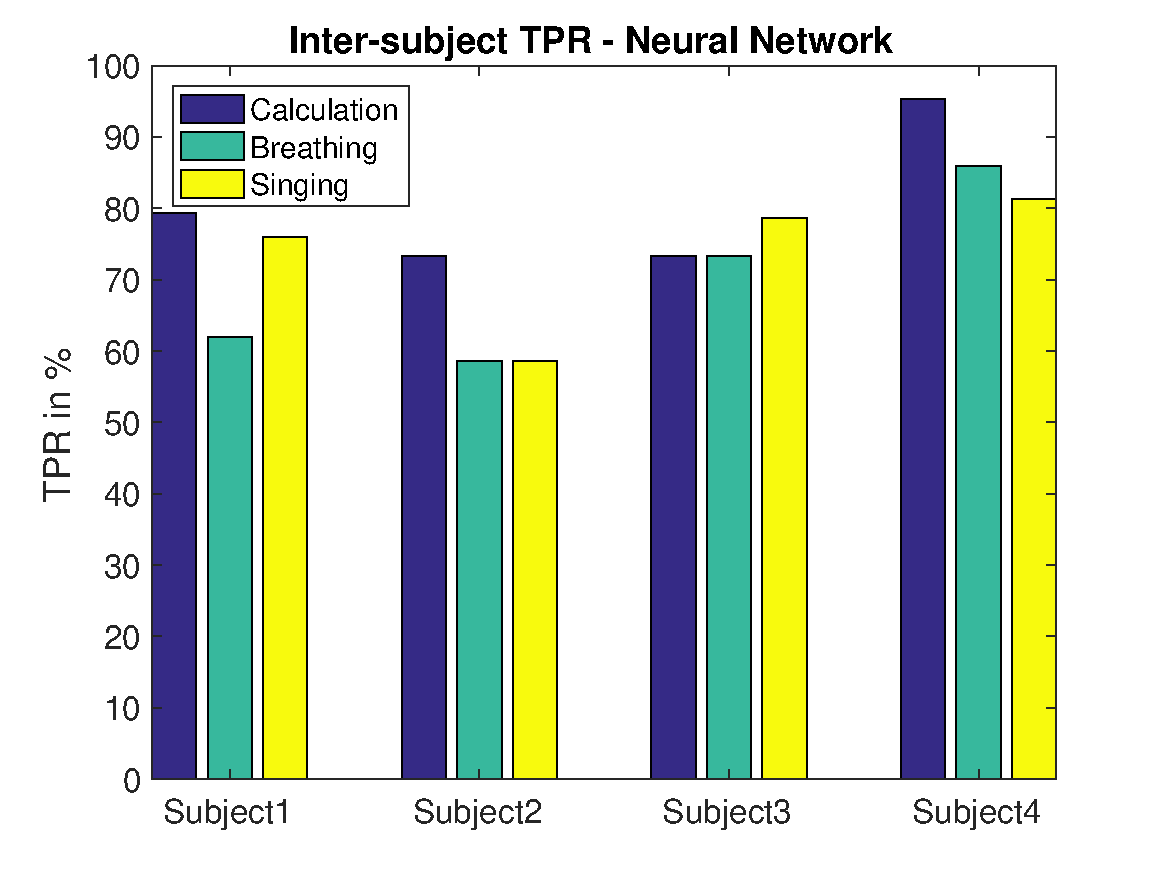
\includegraphics[width=0.90\textwidth]{Chapter-4/base_tprin}
	    	\caption{TPR for Inter-subject classification using Neural Networks}
	    	\label{fig:chap4InterNTPR}
    	\end{figure}

    	\begin{figure}[hbtp]
	    	\centering
	    	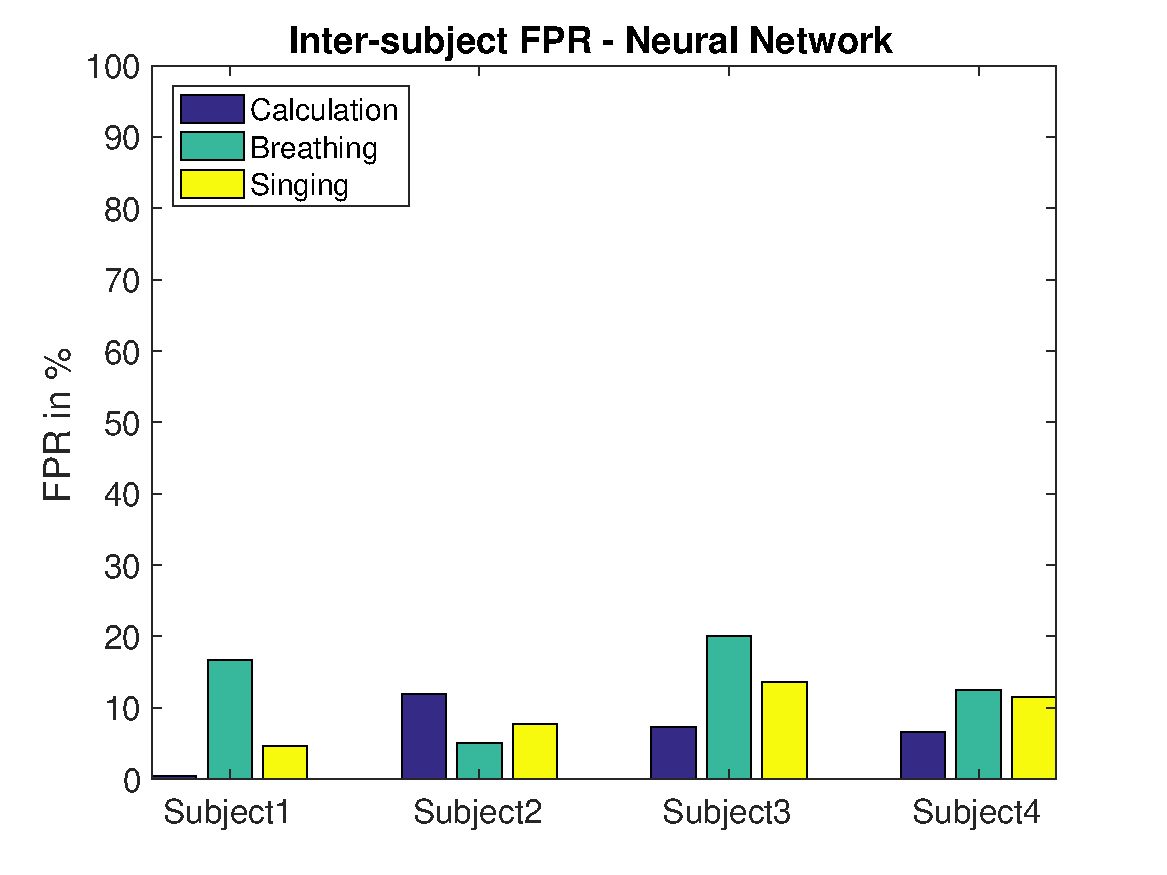
\includegraphics[width=0.90\textwidth]{Chapter-4/base_fprin}
	    	\caption{FPR for Inter-subject classification using Neural Networks}
	    	\label{fig:chap4InterNFPR}
    	\end{figure}

 		\begin{table}[h!]
			\centering
			\caption{Inter-subject Classification for 4 subjects using Neural Networks - TPR for Subject 1-4}
			\label{InNNTPR}
			\subfloat[Subject 1]{
			\begin{tabular}{l c c c}
				\hline
				Task &Min &Max &Average\\\hline
				Calculation &66.67 &86.67 &79.33\\
				Breathing &46.67 &73.33   &62.00\\
				Singing &66.67 &80.00     &76.00\\
			\end{tabular}
			}\hfill
			\subfloat[Subject 2]{
			\begin{tabular}{l c c c}
				\hline
				Task &Min &Max &Average\\\hline
				Calculation &66.67 &93.33 &73.33\\
				Breathing &26.67 &80.00   &58.67\\
				Singing &26.67 &80.00     &58.67\\
			\end{tabular}
			}\\		
			\subfloat[Subject 3]{
			\begin{tabular}{l c c c}
				\hline
				Task &Min &Max &Average\\\hline
				Calculation &60.00 &80.00 &73.33\\
				Breathing &60.00 &86.67   &73.33\\
				Singing &66.67 &93.33     &78.67\\
			\end{tabular}
			}\hfill
			\subfloat[Subject 4]{
			\begin{tabular}{l c c c}
				\hline
				Task &Min &Max &Average\\\hline
				Calculation &86.67 &100.00 &95.33\\
				Breathing &73.33 &100.00   &86.00\\
				Singing &66.67 &100.00     &81.33\\
			\end{tabular}
			}			
		\end{table}
        
		\begin{table}[h!]
			\centering
			\caption{Inter-subject Classification for 4 subjects using Neural Networks - FPR for Subject 1-4}
			\label{InNNFPR}
			\subfloat[Subject 1]{
			\begin{tabular}{l c c c}
				\hline
				Task &Min &Max &Average\\\hline
				Calculation &0.00 &2.22 &0.44\\
				Breathing &8.89 &22.22  &16.67\\
				Singing &2.22 &8.89     &4.67\\
			\end{tabular}
			}\hfill
			\subfloat[Subject 2]{
			\begin{tabular}{l c c c}
				\hline
				Task &Min &Max &Average\\\hline
				Calculation &4.44 &15.56 &12.00\\
				Breathing &0.00 &15.56   &5.11\\
				Singing &2.22 &13.33     &7.78\\
			\end{tabular}
			}\\		
			\subfloat[Subject 3]{
			\begin{tabular}{l c c c}
				\hline
				Task &Min &Max &Average\\\hline
				Calculation &0.00 &13.33 &7.33\\
				Breathing &13.33 &24.44  &20.00\\
				Singing &8.89 &17.78     &13.56\\
			\end{tabular}
			}\hfill
			\subfloat[Subject 4]{
			\begin{tabular}{l c c c}
				\hline
				Task &Min &Max &Average\\\hline
				Calculation &0.00 &11.11 &6.67\\
				Breathing &6.67 &22.22   &12.44\\
				Singing &6.67 &17.78     &11.56\\
			\end{tabular}
			}		
		\end{table}
        
        Inter-subject classification using Neural Networks show more consistency with TPR and FPR compared to Mahalanobis Distance. Also, the TPR and classification accuracy for calculation task is higher compared to breathing and song tasks.
        
        \FloatBarrier
		\subsubsection{Support Vector Machines}
    Table \ref{InSVM} and Figure \ref{fig:chap4InterST} show the overall accuracy of the SVM classifier for inter-subject classification. Table \ref{InSVMTPR} and Figure \ref{fig:chap4InterSTPR} show the TPR for different test subjects using the SVM classifier. Also, Table \ref{InSVMFPR} and Figure \ref{fig:chap4InterSFPR} show the FPR for different test subjects using the SVM classifier.        
		\begin{table}[h!]
			\centering
			\caption{Inter-subject Classification for 4 subjects using Support Vector Machines - Total Accuracy}
			\label{InSVM}
			\begin{tabular}{l c c c}
				\hline
				Task &Min &Max &Average\\\hline
				Calculation &68.33 &80.00 &76.50\\
				Breathing &50.00 &60.00   &55.17\\
				Singing &66.67 &85.00     &75.00\\
			\end{tabular}
		\end{table}

		\begin{figure}[hbtp]
	    	\centering
	    	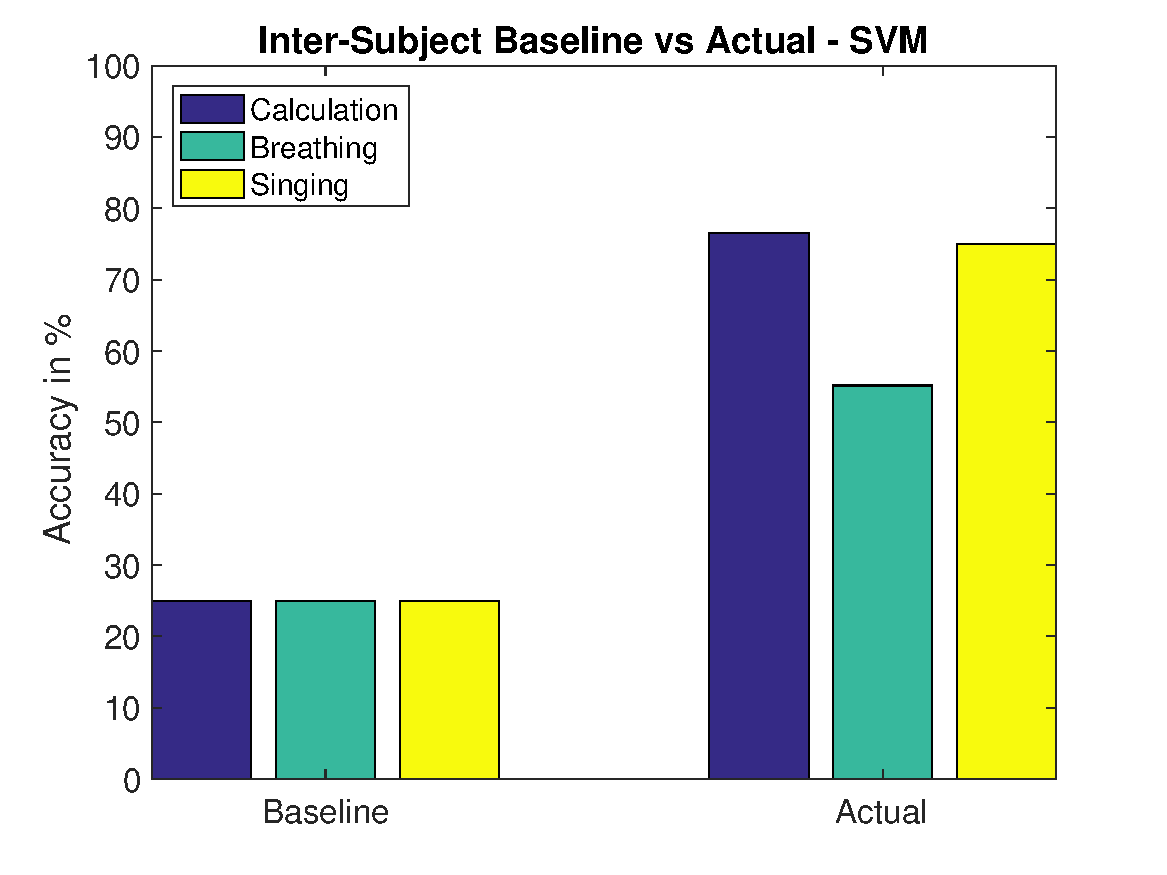
\includegraphics[width=0.90\textwidth]{Chapter-4/base_tis}
	    	\caption{Total accuracy for Inter-subject classification using Support Vector Machines}
	    	\label{fig:chap4InterST}
    	\end{figure}

    	\begin{figure}[hbtp]
	    	\centering
	    	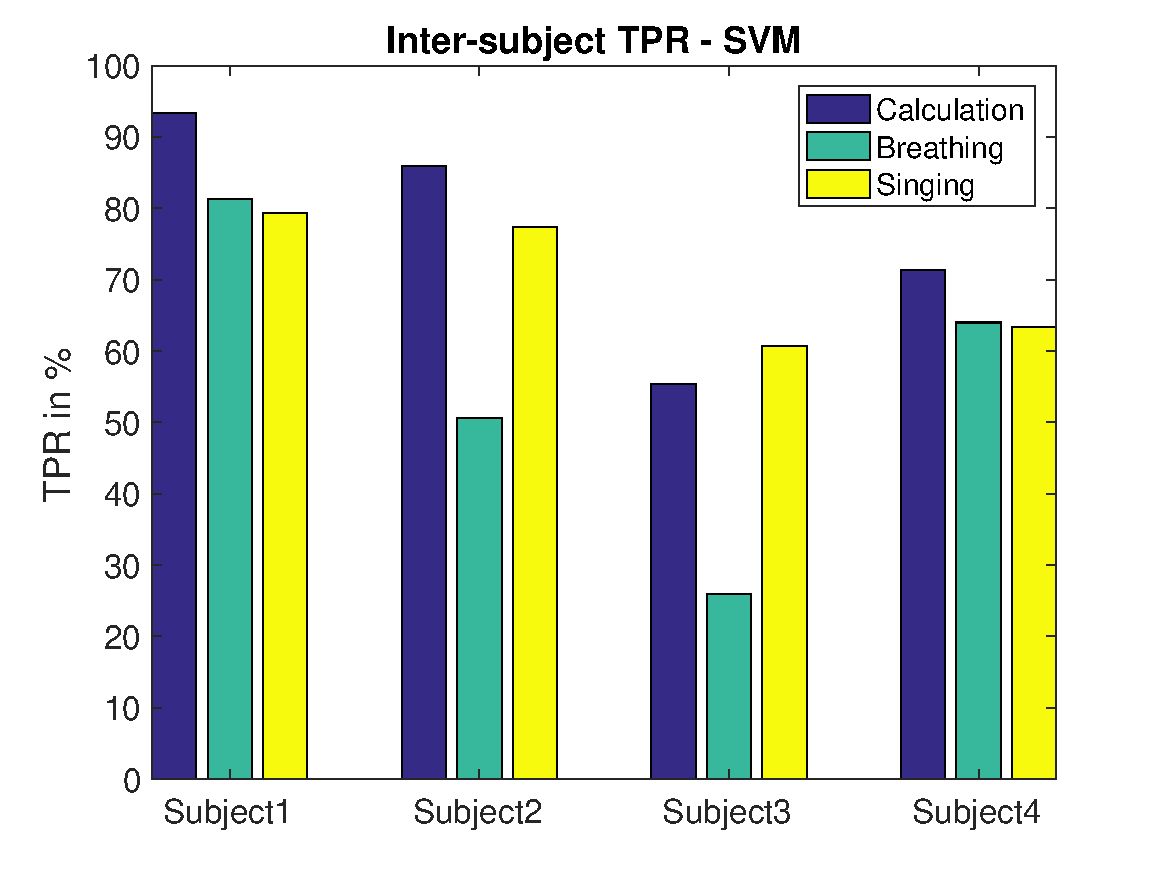
\includegraphics[width=0.90\textwidth]{Chapter-4/base_tpris}
	    	\caption{TPR for Inter-subject classification using Support Vector Machines}
	    	\label{fig:chap4InterSTPR}
    	\end{figure}

    	\begin{figure}[hbtp]
	    	\centering
	    	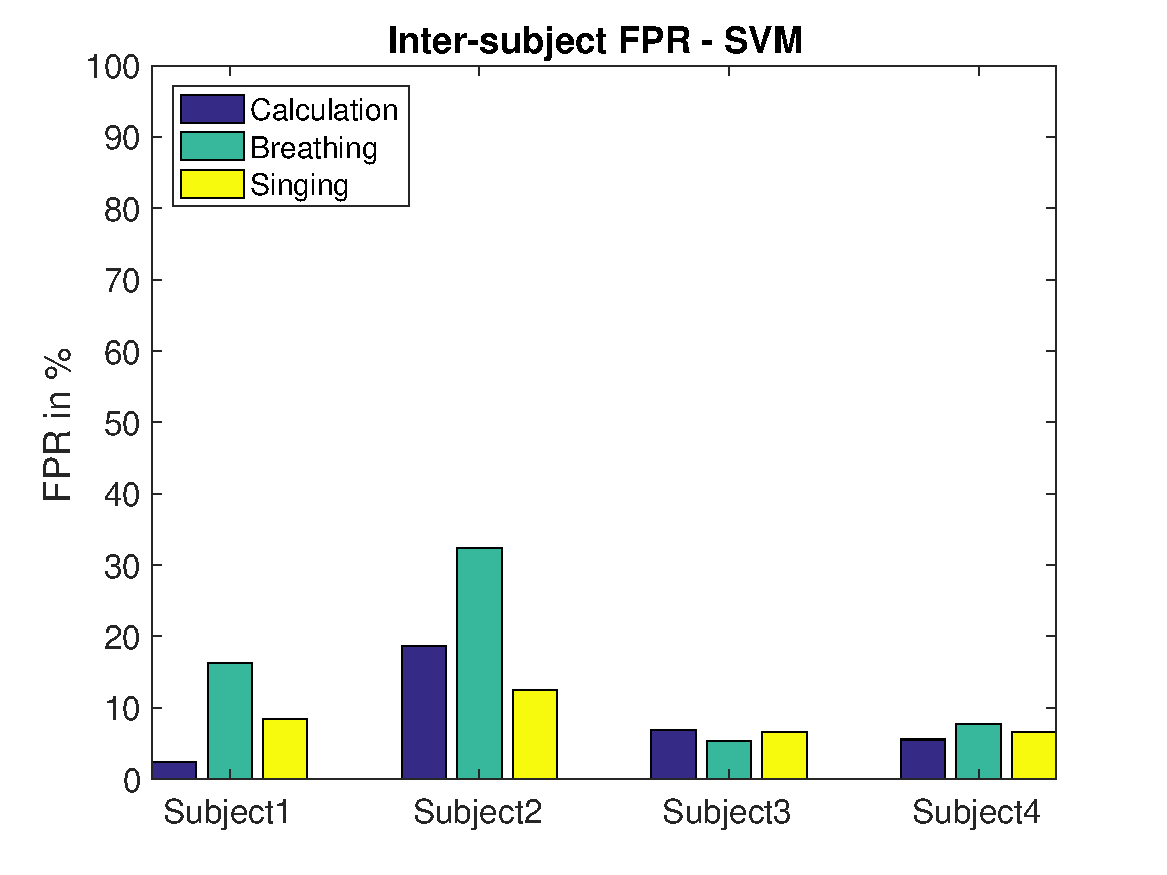
\includegraphics[width=0.90\textwidth]{Chapter-4/base_fpris}
	    	\caption{FPR for Inter-subject classification using Support Vector Machines}
	    	\label{fig:chap4InterSFPR}
    	\end{figure}

        
		\begin{table}[h!]
			\centering
			\caption{Inter-subject Classification for 4 subjects using Support Vector Machines - TPR for Subject 1}
			\label{InSVMTPR}
			\subfloat[Subject 1]{
			\begin{tabular}{l c c c}
				\hline
				Task &Min &Max &Average\\\hline
				Calculation &86.67 &100.00 &93.33\\
				Breathing &66.67 &93.33    &81.33\\
				Singing &60.00 &100.00     &79.33\\
			\end{tabular}
			}
			\subfloat[Subject 2]{
			\begin{tabular}{l c c c}
				\hline
				Task &Min &Max &Average\\\hline
				Calculation &80.00 &100.00 &86.00\\
				Breathing &20.00 &80.00    &50.67\\
				Singing &66.67 &86.67      &77.33\\
			\end{tabular}
			}\\		
			\subfloat[Subject 3]{
			\begin{tabular}{l c c c}
				\hline
				Task &Min &Max &Average\\\hline
				Calculation &40.00 &73.33 &55.33\\
				Breathing &13.33 &33.33   &26.00\\
				Singing &40.00 &73.33     &60.67\\
			\end{tabular}
			}
			\subfloat[Subject 4]{
			\begin{tabular}{l c c c}
				\hline
				Task &Min &Max &Average\\\hline
				Calculation &46.67 &93.33 &71.33\\
				Breathing &46.67 &80.00   &64.00\\
				Singing &33.33 &86.67     &63.33\\
			\end{tabular}
			}
		\end{table}
        
		\begin{table}[h!]
			\centering
			\caption{Inter-subject Classification for 4 subjects using Support Vector Machines - FPR for Subject 1}
			\label{InSVMFPR}
			\subfloat[Subject 1]{
			\begin{tabular}{l c c c}
				\hline
				Task &Min &Max &Average\\\hline
				Calculation &0.00 &6.67 &2.44\\
				Breathing &8.89 &24.44  &16.22\\
				Singing &2.22 &17.78    &8.44\\
			\end{tabular}
			}\hfill
			\subfloat[Subject 2]{
			\begin{tabular}{l c c c}
				\hline
				Task &Min &Max &Average\\\hline
				Calculation &11.11 &31.11 &18.67\\
				Breathing &24.44 &40.00   &32.44\\
				Singing &8.89 &22.22      &12.44\\
			\end{tabular}
			}\\		
			\subfloat[Subject 3]{
			\begin{tabular}{l c c c}
				\hline
				Task &Min &Max &Average\\\hline
				Calculation &2.22 &8.89 &6.89\\
				Breathing &0.00 &13.33  &5.33\\
				Singing &2.22 &11.11    &6.67\\
			\end{tabular}
			}\hfill
			\subfloat[Subject 4]{
			\begin{tabular}{l c c c}
				\hline
				Task &Min &Max &Average\\\hline
				Calculation &0.00 &8.89 &5.56\\
				Breathing &4.44 &17.78  &7.78\\
				Singing &2.22 &15.56    &6.67\\
			\end{tabular}
			}			
		\end{table}

        \FloatBarrier
\ensureoddstart
\chapter{DISCUSSION}
\label{chap-five}

	\section{Classifiers}
		Classification accuracies for both intra-subject and inter-subject classification tests are generally high for Neural Networks and SVMs compared to Mahalanobis Distance. To understand the reason for differing performances of algorithms, we conducted the Henze-Zirkler's Multivariate Normality Test \cite{HZ} \cite{HZart}. The Henze-Zirkler test is based on a non-negative functional distance that measures the distance between two distribution functions. If the data is multivariate normal, the test statistic HZ is approximately lognormally distributed. We calculate the mean, variance and smoothness parameter. Then, the mean and the variance are lognormalized and the p-value is estimated \cite{HZart}. The detailed description of this test can be found in \cite{HZtext}. If the p-value is greater than certain threshold, the distribution is normal. We found that EEG feature vectors from the data collected failed the Henze-Zirkler's Multivariate Normality Test.
        
	\section{Intra-Subject Vs Inter-Subject}
		The intra-subject classification accuracies and TPRs are lower compared to inter-subject classification accuracies. This might be due to similarities in the EEG data for a particular subject. This might also be due to the limitation of the single electrode EEG sensor. For this experiments, the MindWave mobile EEG sensor electrode is placed on the forehead and the ground electrode is placed on the tip of the ear. For this reason, the EEG data from other positions of the human brain are not captured resulting in lack of information to effectively distinguish between different EEG data generated by the same subject. 
	
    \section{Tasks}
    	The classification accuracies and TPR for calculation task was found consistently higher compared to breathing task and song task for all the classifiers used. This might be because the EEG signatures in calculation task are more distinguishable compared the EEG signatures in other tasks. Also note that both breathing task and singing task involved concentrating on breathing and the singing respectively while calculation task involved actual calculation of two digit multiplication. This shows that certain tasks are easily identifiable compared to others.

	\section{Number of classes}
		It was also found that the classification accuracies drop as we increase the number of classes in case inter-subject classification. The baseline performance is given by Equation \ref{EQ:chap4base}. We can see from Figure \ref{fig:chap5calc}, Figure \ref{fig:chap5breath} and Figure \ref{fig:chap5song} that the baseline performance decreases with increase in the number of classes. Also, we can see that the classification performance of Mahalanobis Distance, Neural Network and SVM classifiers are better than the baseline performance. Note that there is performance decrease even after using classifiers when we increase the number of classes, however the decrease in performance is less compared to baseline performance.
		\begin{figure}[hbtp]
	    	\centering
	    	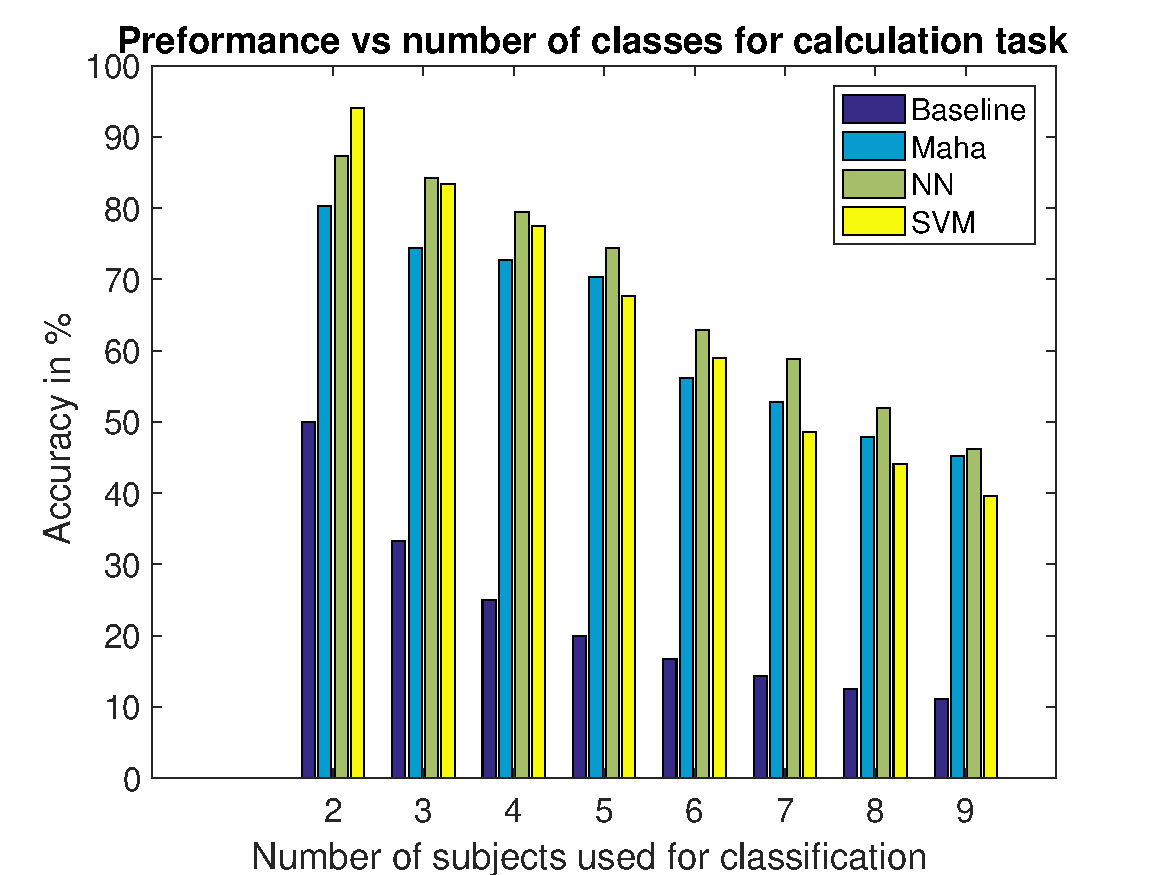
\includegraphics[width=0.9\textwidth]{Chapter-5/calc_base}
	    	\caption{Preformance vs number of classes for calculation task}
	    	\label{fig:chap5calc}
	    \end{figure}
	    
		\begin{figure}[hbtp]
	    	\centering
	    	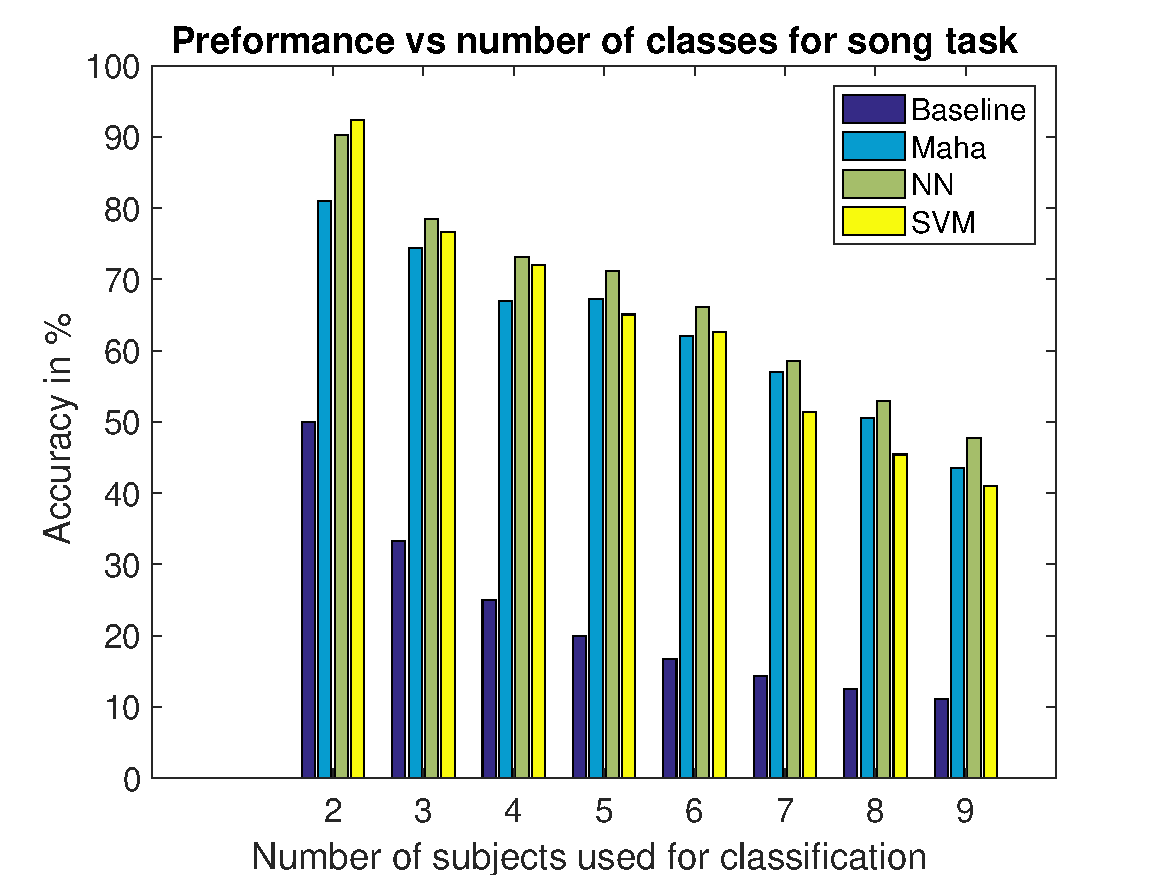
\includegraphics[width=0.9\textwidth]{Chapter-5/breath_base}
	    	\caption{Preformance vs number of classes for breathing task}
	    	\label{fig:chap5breath}
	    \end{figure}

		\begin{figure}[hbtp]
	    	\centering
	    	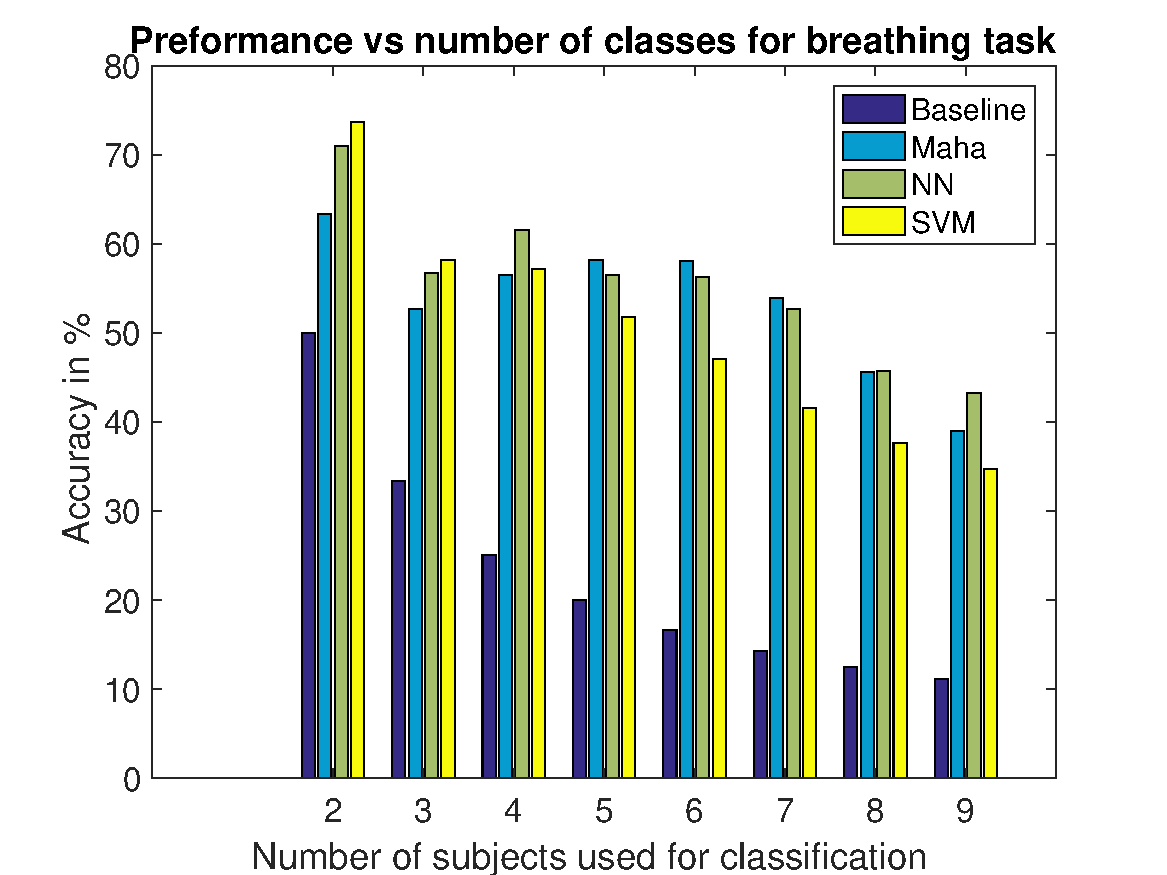
\includegraphics[width=0.9\textwidth]{Chapter-5/song_base}
	    	\caption{Preformance vs number of classes for singing task}
	    	\label{fig:chap5song}
	    \end{figure}
	    \FloatBarrier


    	


%\include{Chapter-6/Chapter-6}
%\restoregeometry

\begin{spacing}{1}
 \setlength\bibitemsep{11pt} %22pt = 2*11pt, where fontsize is 11pt
 \addcontentsline{toc}{chapter}{{\uppercase{\bibname}}} %\textorpdfstring and \uppercase needed due to hyperref package http://www.latex-community.org/forum/viewtopic.php?f=44&t=16601
 %\vspace{-0.5in}
\titleformat{\chapter}[display]{\bf\filcenter
}{\chaptertitlename\ \thechapter}{11pt}{\bf\filcenter}
\titlespacing*{\chapter}{0pt}{-0.5in-9pt}{22pt}

\printbibliography[heading=myheading]
\end{spacing}

% Appendices
\restoregeometry
\appendix
\newgeometry{margin=1in,lmargin=1.25in,footskip=\chapterfootskip, includehead, includefoot}

\setstretch{1.0}
\ensureoddstart
\chapter{Matlab Code}

This Appendix includes Matlab code for the EEG security.
\pagebreak


\noindent Filename : getFeatures.m
\lstinputlisting[language=Octave]{Appendix-A/getFeatures.m}
\pagebreak
Filename : prepareData.m
\lstinputlisting[language=Octave]{Appendix-A/prepareData.m}
\pagebreak
Filename : shuffleData.m
\lstinputlisting[language=Octave]{Appendix-A/shuffleData.m}
\pagebreak
Filename : performance.m
\lstinputlisting[language=Octave]{Appendix-A/performance.m}
\pagebreak
Filename : interTests.m
\lstinputlisting[language=Octave]{Appendix-A/interTests.m}
\pagebreak
Filename : intraTests.m
\lstinputlisting[language=Octave]{Appendix-A/intraTests.m}
\pagebreak
Filename : mahaIntra.m
\lstinputlisting[language=Octave]{Appendix-A/mahaIntra.m}
\pagebreak
Filename : mahaInter.m
\lstinputlisting[language=Octave]{Appendix-A/mahaInter.m}
\pagebreak
Filename : get\_maha\_features.m
\lstinputlisting[language=Octave]{Appendix-A/get_maha_features.m}
\pagebreak
Filename : get\_maha\_dist.m
\lstinputlisting[language=Octave]{Appendix-A/get_maha_dist.m}
\pagebreak
Filename : nnIntra.m
\lstinputlisting[language=Octave]{Appendix-A/nnIntra.m}
\pagebreak
Filename : nnInter.m
\lstinputlisting[language=Octave]{Appendix-A/nnInter.m}
\pagebreak
Filename : sigmoid.m
\lstinputlisting[language=Octave]{Appendix-A/sigmoid.m}
\pagebreak
Filename : sigmoidGradient.m
\lstinputlisting[language=Octave]{Appendix-A/sigmoidGradient.m}
\pagebreak
Filename : randInitializeWeights.m
\lstinputlisting[language=Octave]{Appendix-A/randInitializeWeights.m}
\pagebreak
Filename : nnCostFunction.m
\lstinputlisting[language=Octave]{Appendix-A/nnCostFunction.m}
\pagebreak
Filename : predict.m
\lstinputlisting[language=Octave]{Appendix-A/predict.m}
\pagebreak
Filename : fmincg.m
\lstinputlisting[language=Octave]{Appendix-A/fmincg.m}

\ensureoddstart
\chapter{Python Code}

This Appendix includes Python code for the EEG security.
\pagebreak

\noindent Filename : main.py
\lstinputlisting[language=Python]{Appendix-B/main.py}
\pagebreak
Filename : pre\_process.py
\lstinputlisting[language=Python]{Appendix-B/pre_process.py}
\pagebreak
Filename : mindwave.py
\lstinputlisting[language=Python]{Appendix-B/mindwave.py}
\pagebreak
Filename : classifiers.py
\lstinputlisting[language=Python]{Appendix-B/classifiers.py}
\pagebreak
Filename : tests.py
\lstinputlisting[language=Python]{Appendix-B/tests.py}



\restoregeometry

\backmatter


\end{document}
